\documentclass[11pt,a4paper]{article}
\usepackage[utf8]{inputenc}
\usepackage[T1]{fontenc}
\usepackage[spanish,es-noshorthands]{babel}
\usepackage{geometry}
\geometry{margin=2.6cm}
\usepackage{calc}
\usepackage{longtable}
\usepackage{booktabs}
\usepackage{array}
\usepackage{ragged2e}
\usepackage{graphicx}
\usepackage{float}
\usepackage[table]{xcolor}
\usepackage{caption}
\captionsetup{skip=6pt}
\usepackage{titlesec}
\usepackage{fancyhdr}
\usepackage[hidelinks]{hyperref}
\usepackage{enumitem}
\usepackage{parskip}
\usepackage{needspace}
\usepackage{etoolbox}
\setlength{\parskip}{0.55em}
\setlist{itemsep=0.2em}

% evita titulos "huerfanos" solos al final de una pagina, empujandolos a la
% siguiente si no queda espacio para el titulo mas unas lineas de contenido
\pretocmd{\section}{\needspace{5\baselineskip}}{}{}
\pretocmd{\subsection}{\needspace{4\baselineskip}}{}{}
\pretocmd{\subsubsection}{\needspace{3\baselineskip}}{}{}

% --- Macros pandoc espera que existan (normalmente las inyecta su modo -s) ---
\providecommand{\tightlist}{%
  \setlength{\itemsep}{0pt}\setlength{\parskip}{0pt}}
\providecommand{\pandocbounded}[1]{#1}
\newcommand{\passthrough}[1]{#1}

\hypersetup{
  pdftitle={HemoScan Andino},
  pdfauthor={Equipo HemoScan Andino -- UPeU Juliaca},
  colorlinks=false,
  bookmarksopen=true
}

% El contenido ya trae su propia numeracion manual (1., 1.1, 1.1.1...) escrita
% en el texto de cada encabezado, asi que se desactiva la numeracion automatica
% de LaTeX para evitar una doble numeracion en el indice y en el cuerpo.
\setcounter{secnumdepth}{-2}
\setcounter{tocdepth}{4}
\titleformat{\section}{\normalfont\Large\bfseries}{}{0em}{}
\titleformat{\subsection}{\normalfont\large\bfseries}{}{0em}{}
\titleformat{\subsubsection}{\normalfont\normalsize\bfseries}{}{0em}{}

% Encabezado con dos etiquetas CORTAS y de ancho fijo (nunca texto largo o
% dinamico por subseccion) para que jamas puedan solaparse entre si.
\pagestyle{fancy}
\fancyhf{}
\fancyhead[L]{\small HemoScan Andino}
\fancyhead[R]{\small Software E1 --- Requerimientos}
\fancyfoot[C]{\thepage}
\renewcommand{\headrulewidth}{0.4pt}

\begin{document}

\begin{titlepage}
\centering
\vspace*{1.2cm}
{\large UNIVERSIDAD PERUANA UNI\'ON\par}
{\normalsize Facultad de Ingenier\'ia y Arquitectura\par}
{\normalsize Escuela Profesional de Ingenier\'ia de Sistemas --- Filial Juliaca\par}
\vspace{0.5cm}
\rule{0.6\linewidth}{0.4pt}
\vspace{1.6cm}

{\large PROYECTO DE TESIS / PROYECTO INTEGRADOR\par}
\vspace{1.0cm}
{\huge\bfseries HemoScan Andino\par}
\vspace{0.6cm}
{\Large Sistema no invasivo de tamizaje de anemia infantil con fusi\'on \'optica multisensor y autocalibraci\'on por altitud\par}
\vspace{1.6cm}
\rule{0.6\linewidth}{0.4pt}
\vspace{1.6cm}

{\Large\bfseries Entregable 1 de Software (CE021) --- Requerimientos y Dise\~no del Sistema\par}
\vspace{2.0cm}

{\normalsize Juliaca, Puno, Per\'u \par}
{\normalsize Julio de 2026\par}

\vfill
\end{titlepage}

\tableofcontents
\newpage

\textbf{Entregable N.° 5 --- Requerimientos y Diseño del Sistema}
\emph{(Quinto entregable consecutivo del proyecto HemoScan Andino. Corresponde al Entregable N.° 1 de la competencia CE021 --- Área C: Ingeniería de Software; utiliza una numeración de Entregable propia y distinta de la de los Entregables N.° 1-4 del Área B ya presentados, aunque continúa la secuencia documental del proyecto)}

\textbf{Área de competencia:} Área C --- Ingeniería de Software
\textbf{Competencia:} CE021 --- Ingeniería de Requerimientos
\textbf{Evidencia que cubre este documento:} CE021 (Especificación de Requerimientos, Prototipo Navegable, Diseño Arquitectónico y Diseño Detallado del sistema HemoScan Andino)
\textbf{Sistema documentado:} HemoScan Andino --- aplicación móvil Flutter/PWA offline-first, backend de interoperabilidad FHIR (FastAPI/NestJS), modelo de inferencia multimodal embebido (ONNX/TFLite) y plataforma web de analítica geoespacial (React/TypeScript)

\textbf{Organización diagnosticada (caso ilustrativo y representativo):} Microred de Salud Altiplano-Puno

\begin{center}\rule{0.5\linewidth}{0.5pt}\end{center}

\textbf{Integrantes del equipo:}

{\small
\begin{longtable}[]{@{}
  >{\raggedright\arraybackslash}p{(\linewidth - 4\tabcolsep) * \real{0.3333}}
  >{\raggedright\arraybackslash}p{(\linewidth - 4\tabcolsep) * \real{0.3333}}
  >{\raggedright\arraybackslash}p{(\linewidth - 4\tabcolsep) * \real{0.3333}}@{}}
\toprule\noalign{}
\begin{minipage}[b]{\linewidth}\raggedright
N.°
\end{minipage} & \begin{minipage}[b]{\linewidth}\raggedright
Integrante
\end{minipage} & \begin{minipage}[b]{\linewidth}\raggedright
Rol / Área de competencia
\end{minipage} \\
\midrule\noalign{}
\endhead
\bottomrule\noalign{}
\endlastfoot
1 & \textbf{{[}DATO PENDIENTE DE VALIDAR: nombre completo del Integrante 1, Líder de Infraestructura Tecnológica{]}} & CE03 --- Infraestructura Tecnológica (red, seguridad, centro de datos) \\
2 & \textbf{{[}DATO PENDIENTE DE VALIDAR: nombre completo del Integrante 2, Líder de Gestión de TI{]}} & CE01 --- Gestión de TI (diagnóstico, business case, plan de gestión, procesos) \\
3 & \textbf{{[}DATO PENDIENTE DE VALIDAR: nombre completo del Integrante 3, Líder de Ingeniería de Software{]}} & CE02 --- Ingeniería de Software (requerimientos, datos, sistema, calidad) --- \textbf{responsable principal de este entregable} \\
\end{longtable}
}

\textbf{Docente asesor(a) del curso:} \textit{(nombre del docente asesor por completar)}
\textbf{Curso / Sílabo:} \textit{(nombre del curso / s\'ilabo por completar)}
\textbf{Ciclo académico:} 2026-I (supuesto, a confirmar con la programación académica vigente)

\begin{quote}
\textbf{Nota de honestidad sobre la portada.} La plantilla del producto de la competencia CE021 exige consignar en la portada el nombre real de cada estudiante. Al momento de este entregable dicho dato no ha sido provisto al equipo redactor ni puede derivarse razonablemente de los entregables anteriores, por lo que ---siguiendo la misma disciplina de honestidad técnica del resto del documento--- se marca explícitamente como \textbf{{[}DATO PENDIENTE DE VALIDAR{]}} en lugar de sustituirse por un nombre inventado. Esta portada debe completarse con los nombres reales de los tres integrantes, como mínimo, antes de la entrega final del entregable.
\end{quote}

\textbf{Lugar y fecha:} Juliaca, Puno, Perú --- 07 de julio de 2026

\begin{center}\rule{0.5\linewidth}{0.5pt}\end{center}

\begin{quote}
\textbf{Nota metodológica y alcance (léase antes de continuar).} Este documento es el Entregable N.° 5 del proyecto HemoScan Andino y se apoya directamente en los cuatro entregables precedentes: el \textbf{Entregable N.° 1} (Diagnóstico Organizacional), del cual toma el problema central, los usuarios y la cadena de valor; el \textbf{Entregable N.° 2} (Business Case), del cual toma el modelo de negocio de 3 fases y las cifras de costeo unitario; el \textbf{Entregable N.° 3} (Plan de Gestión del Proyecto), del cual toma íntegramente la Estructura de Desglose del Trabajo de la rama 4 (Ingeniería de Software), el registro de riesgos y, en particular, el \textbf{product backlog de 25 historias de usuario (HD01-HD08, HC01-HC17) en 8 épicas}, que aquí se referencia y se cruza con los requerimientos formales en lugar de duplicarse íntegramente; y el \textbf{Entregable N.° 4} (Modelado de Procesos AS-IS/TO-BE), del cual toma como insumo directo \textbf{las catorce automatizaciones propuestas (A1-A14)} y la matriz de trazabilidad FHIR por etapa (su Anexo E), que constituyen la base declarada para derivar los requerimientos funcionales de este documento. Se mantiene vigente la misma advertencia metodológica de los cuatro entregables anteriores: HemoScan Andino \textbf{no cuenta todavía con un convenio real} con ninguna microred o posta de salud, por lo que este documento diseña el sistema para la organización \textbf{ilustrativa y representativa ``Microred de Salud Altiplano-Puno''}. Adicionalmente, y de forma específica para este entregable, se declaran tres límites de honestidad técnica adicionales. Primero, \textbf{no se dispone de herramientas de modelado gráfico propietarias con licencia (Figma, Enterprise Architect)}; siguiendo la misma convención de \emph{diagrama-como-código} (\emph{diagram-as-code}) ya establecida en el Entregable N.° 4, todos los diagramas de este documento se especifican como texto abierto y gratuito y se \textbf{renderizan a imagen vectorial mediante un renderizador libre de licencia} (Mermaid, ejecutado con \texttt{mermaid-cli}), incorporándose al cuerpo del documento como figuras. Por este medio se generan tanto los diagramas núcleo del diseño detallado en notación UML ---casos de uso, clases, los cuatro diagramas de secuencia y los tres diagramas de estados (sección 4)--- como las vistas complementarias de navegación, arquitectura, componentes, despliegue, relaciones FHIR y paquetes. A diferencia de una revisión previa de este entregable, que dejaba pendiente la ejecución del renderizador y presentaba los diagramas en cajas de texto ASCII, en esta versión dicha verificación \textbf{sí se ejecutó}: cada diagrama fue renderizado sin errores de sintaxis y su imagen vectorial es la que aparece a continuación en cada sección. Segundo, el \textbf{prototipo navegable de la sección 2 es de fidelidad media, presentado como mockups renderizados de las pantallas}, no un artefacto interactivo clicable; esta limitación se declara explícitamente y se retoma en la autoevaluación final. Tercero, \textbf{los parámetros clínicos exactos de la NTS 213-MINSA/DGIESP-2024} (puntos de corte de hemoglobina por edad, fórmula o tabla exacta de corrección por altitud, posología de hierro) no estuvieron disponibles en su texto íntegro y vigente al momento de este entregable ---la misma limitación ya declarada en el Entregable N.° 4---, por lo que el sistema se diseña deliberadamente para \textbf{parametrizar y versionar} estos valores en lugar de fijarlos (``hardcodearlos''), y cada valor numérico específico que no pueda derivarse razonablemente de lo ya declarado en el proyecto se marca de forma explícita como \textbf{{[}DATO PENDIENTE DE VALIDAR{]}}.
\end{quote}

\begin{center}\rule{0.5\linewidth}{0.5pt}\end{center}

\section{Resumen Ejecutivo}\label{resumen-ejecutivo}

Puno registra la prevalencia de anemia infantil más alta del Perú (56.1 \% en menores de 3 años, ENDES 2025 --- cifra oficial ya validada en el Entregable N.° 1), en un contexto donde el método de referencia (HemoCue, punción capilar) es invasivo y de acceso limitado en zonas rurales, y donde la corrección de hemoglobina por altitud a 3,800 msnm puede inducir sobrediagnóstico si no se aplica de forma auditable (Gonzales et al.~2025; Baquerizo-Sedano et al.~2025). Sobre esta base, ya diagnosticada y modelada en los Entregables N.° 1 y N.° 4, el presente Entregable N.° 5 desarrolla la \textbf{Ingeniería de Requerimientos (CE021)} del sistema HemoScan Andino: una aplicación móvil Flutter/PWA offline-first que opera junto a un nodo de hardware (ESP32-S3, AS7341, MAX30102, LED blanco alto CRI) mediante Bluetooth Low Energy, un modelo de inferencia multimodal embebido (ONNX/TFLite) con una capa independiente y auditable de autocalibración por altitud (GPS + Modelo Digital de Elevación, nunca altitud cruda de GPS), un backend de interoperabilidad FHIR (FastAPI o NestJS, sobre PostgreSQL/PostGIS) que sincroniza de forma diferida con el HIS-MINSA y el Padrón Nominal, y una plataforma web (React/TypeScript) de analítica geoespacial para la Jefatura de microred y la DIRESA/GERESA.

Los \textbf{usuarios} del sistema abarcan un espectro humano y organizacional completo: el personal de Crecimiento y Desarrollo (CRED) que opera el dispositivo en campo, el personal médico que confirma o descarta el diagnóstico (decisión que el sistema nunca automatiza, en cumplimiento estricto del DS 115-2025-PCM), el cuidador o cuidadora que otorga el consentimiento informado y recibe la consejería y los recordatorios, el personal de farmacia que gestiona el stock de hierro, y la Jefatura de microred junto con analistas de la DIRESA/GERESA que consumen analítica agregada y anonimizada para la planificación de salud pública. El \textbf{alcance} de este entregable comprende cuatro artefactos exigidos por la competencia CE021: (1) una especificación de requerimientos funcionales (40 RF), no funcionales (20 RNF), reglas de negocio (12 RN) y restricciones, con 11 casos de uso formalmente desarrollados y trazables a las 14 automatizaciones del Entregable N.° 4 y a las 25 historias de usuario del Entregable N.° 3; (2) un prototipo navegable de 16 pantallas de aplicación móvil y 7 pantallas de plataforma web, descrito mediante wireframes textuales y un mapa de navegación completo, con evidencia de una validación heurística interna; (3) un diseño arquitectónico compuesto por un diagrama de componentes, un diagrama de despliegue y un registro de 10 decisiones arquitectónicas (ADR) que resuelven explícitamente las disyuntivas dejadas abiertas por el enunciado del proyecto (FastAPI vs.~NestJS, ONNX Runtime vs.~TFLite, alcance de recursos FHIR, activación de la telemedicina y del aprendizaje federado); y (4) un diseño detallado en notación UML textual, con diagrama de casos de uso, diagrama de clases de 20 entidades, cuatro diagramas de secuencia, tres diagramas de estados y el modelo de datos detallado con su mapeo a los seis recursos FHIR del proyecto.

La \textbf{solución} aquí especificada y diseñada preserva, como principio rector transversal a todos los artefactos del documento, que HemoScan Andino es un \textbf{sistema de tamizaje que deriva a confirmación clínica humana, nunca un diagnóstico autónomo} ---principio ya establecido en el Entregable N.° 1 y reafirmado en el Entregable N.° 4---, y que toda automatización debe quedar registrada de forma auditable, en cumplimiento del reglamento de inteligencia artificial en salud (DS 115-2025-PCM) y de la Ley N.° 29733 de Protección de Datos Personales, dada la máxima sensibilidad de tratarse de datos de salud de menores de edad. El documento cierra con una autoevaluación honesta frente a la rúbrica de seis criterios, reconociendo que la especificación de requerimientos, la trazabilidad y el diseño arquitectónico son ejercicios enteramente completables en gabinete con la información ya disponible en los entregables anteriores, mientras que la validación con stakeholders reales ---por ausencia de convenio institucional y de usuarios finales accesibles--- es la limitación más severa y honesta de este entregable.

\begin{center}\rule{0.5\linewidth}{0.5pt}\end{center}

\subsection{Introducción y alcance del documento}\label{introducciuxf3n-y-alcance-del-documento}

Este documento constituye el Entregable N.° 5 del proyecto HemoScan Andino y evalúa específicamente la competencia \textbf{CE021 --- Ingeniería de Requerimientos}, bajo la responsabilidad principal del Integrante 3 (Líder de Ingeniería de Software), con dos dependencias explícitas de coordinación: hacia el Integrante 1 (Infraestructura Tecnológica), responsable de validar la factibilidad de red, energía y seguridad de los dos escenarios de conectividad que este diseño asume (con y sin cobertura, ya cuantificados en la sección 4.3.1 del Entregable N.° 4); y hacia el Integrante 2 (Gestión de TI), cuyo Plan de Gestión (Entregable N.° 3) fija el cronograma de 8 sprints y el presupuesto dentro de los cuales debe construirse lo aquí especificado.

El alcance de este entregable se circunscribe a los cuatro artefactos que exige la Plantilla del Producto de la rúbrica CE021: especificación de requerimientos, prototipo navegable, diseño arquitectónico y diseño detallado. Deliberadamente \textbf{no} se incluye en este documento código fuente, resultados de pruebas ejecutadas ni métricas de un sistema en funcionamiento ---esa evidencia corresponde al paquete EDT 4.7 (Aseguramiento de la calidad) y a la validación de campo del Mes 7, ninguno de los cuales ha ocurrido a la fecha---. Este entregable es, por diseño, un ejercicio de ingeniería \emph{previo a la construcción}, cuyo propósito es que el sistema no se construya ``sobre la marcha'' sino a partir de una especificación validada internamente, trazable y arquitectónicamente fundamentada.

Para representar los prototipos y diagramas sin herramientas gráficas propietarias, este entregable adopta consistentemente la disciplina de \emph{diagrama-como-código}: cada diagrama se especifica como texto (notación Mermaid) y se renderiza a imagen vectorial con un renderizador libre de licencia, incorporándose como figura. Se cubren así los wireframes del prototipo (como mockups renderizados), los diagramas de arquitectura, y la notación estándar de UML (actor-caso de uso, clase-atributo-relación, línea de vida-mensaje, estado-transición) para el diseño detallado. Se incluye una leyenda antes del primer diagrama de cada tipo.

\begin{center}\rule{0.5\linewidth}{0.5pt}\end{center}

\section{1. Especificación de Requerimientos}\label{especificaciuxf3n-de-requerimientos}

\subsection{1.1 Visión general del sistema y actores}\label{visiuxf3n-general-del-sistema-y-actores}

HemoScan Andino, desde la perspectiva de la Ingeniería de Software, se compone de cuatro subsistemas que interactúan de forma offline-first (ninguno depende de conectividad permanente para su función crítica):

\begin{enumerate}
\def\labelenumi{\arabic{enumi}.}
\tightlist
\item
  \textbf{Firmware y nodo de hardware} (ESP32-S3 + AS7341 + MAX30102 + LED blanco alto CRI): captura las tres señales ópticas y las transmite por BLE. No forma parte del alcance de construcción del Integrante 3 en solitario (EDT 4.3, compartido con el Integrante 1), pero sí de su especificación de requerimientos, por ser el origen de los datos que todo el resto del sistema procesa.
\item
  \textbf{Aplicación móvil} (Flutter/PWA, offline-first): opera el flujo completo de tamizaje, consentimiento, resultado, consejería, recordatorios y confirmación clínica en campo.
\item
  \textbf{Backend de interoperabilidad} (FastAPI o NestJS, monolito modular sobre PostgreSQL/PostGIS): genera y persiste los recursos FHIR, sincroniza con sistemas externos, coordina el aprendizaje federado y sirve a la plataforma web.
\item
  \textbf{Plataforma web} (React/TypeScript): expone el mapa de cobertura/riesgo geoespacial, reportes agregados y la administración del sistema a la Jefatura de microred, la DIRESA/GERESA y el administrador.
\end{enumerate}

La siguiente tabla presenta los \textbf{actores} del sistema, humanos y no humanos, que se utilizan de forma consistente en los casos de uso (sección 1.6) y en los diagramas UML (sección 4):

{\small
\begin{longtable}[]{@{}
  >{\raggedright\arraybackslash}p{(\linewidth - 4\tabcolsep) * \real{0.3333}}
  >{\raggedright\arraybackslash}p{(\linewidth - 4\tabcolsep) * \real{0.3333}}
  >{\raggedright\arraybackslash}p{(\linewidth - 4\tabcolsep) * \real{0.3333}}@{}}
\toprule\noalign{}
\begin{minipage}[b]{\linewidth}\raggedright
Actor
\end{minipage} & \begin{minipage}[b]{\linewidth}\raggedright
Descripción
\end{minipage} & \begin{minipage}[b]{\linewidth}\raggedright
Tipo de interacción principal
\end{minipage} \\
\midrule\noalign{}
\endhead
\bottomrule\noalign{}
\endlastfoot
Cuidador/a (madre, padre o tutor) & Persona responsable del niño o niña tamizado; otorga el consentimiento informado y recibe consejería/recordatorios & Interacción ocasional vía app (consentimiento, notificaciones); Lane 1 en el Entregable N.° 4 \\
Personal CRED / técnico de salud & Opera el dispositivo y la app durante el control de Crecimiento y Desarrollo & Uso intensivo de la app móvil en campo; Lane 2/3 en el Entregable N.° 4 \\
Personal médico & Realiza la confirmación clínica y la prescripción; único actor habilitado para ambas decisiones (RN-06) & App móvil o módulo web de confirmación, presencial o por telemedicina (extensión evaluada en 1.9); Lane 4 \\
Personal de farmacia/almacén & Gestiona la dispensación y el stock de insumos de hierro (integración con SIGA) & Interacción indirecta mediante alertas del sistema; Lane 5 \\
Jefatura de microred & Supervisa throughput, cobertura y desempeño agregado de la microred & Plataforma web (dashboard, mapa, reportes) \\
Analista DIRESA/GERESA & Consume analítica agregada y anonimizada para planificación regional & Plataforma web, con alcance entre microredes (Fase 1/2) \\
Administrador del sistema & Gestiona usuarios, roles y parámetros de configuración clínica (p.~ej., tabla de corrección por altitud) & Consola de administración de la plataforma web \\
Auditor / Comité de ética (rol externo) & Verifica cumplimiento normativo mediante consulta de trazas de auditoría & Plataforma web, solo lectura, alcance restringido \\
Sistema externo --- HIS-MINSA / Padrón Nominal & Actor no humano; consume/provee recursos FHIR & Integración API FHIR REST, en modo diferido \\
Sistema externo --- SIGA & Actor no humano; consumidor de alertas de stock & Integración vía API o archivo de intercambio --- \textbf{{[}DATO PENDIENTE DE VALIDAR: mecanismo exacto de integración con SIGA; no especificado en el enunciado del proyecto{]}} \\
Dispositivo HemoScan Andino (nodo) & Actor no humano; genera las señales ópticas crudas & Integración BLE con la app móvil \\
Coordinador de aprendizaje federado (Flower) & Actor no humano; orquesta el reentrenamiento distribuido del modelo entre postas & Interno al backend; no activo en Fase 0 (ver ADR-08) \\
\end{longtable}
}

\subsection{1.2 Requerimientos funcionales (RF)}\label{requerimientos-funcionales-rf}

Los 40 requerimientos funcionales se agrupan en ocho módulos, cada uno trazable a una o más de las 14 automatizaciones (A1-A14) del Entregable N.° 4. La columna ``Automatización'' usa el prefijo A\# definido en dicho entregable; donde un requerimiento es una condición habilitante transversal (no una automatización nombrada explícitamente), se indica como tal. La prioridad sigue la escala MoSCoW ya utilizada en el backlog del Entregable N.° 3.

\textbf{Módulo M1 --- Captura y firmware del nodo}

{\small
\begin{longtable}[]{@{}
  >{\raggedright\arraybackslash}p{(\linewidth - 6\tabcolsep) * \real{0.2500}}
  >{\raggedright\arraybackslash}p{(\linewidth - 6\tabcolsep) * \real{0.2500}}
  >{\raggedright\arraybackslash}p{(\linewidth - 6\tabcolsep) * \real{0.2500}}
  >{\raggedright\arraybackslash}p{(\linewidth - 6\tabcolsep) * \real{0.2500}}@{}}
\toprule\noalign{}
\begin{minipage}[b]{\linewidth}\raggedright
ID
\end{minipage} & \begin{minipage}[b]{\linewidth}\raggedright
Requerimiento funcional
\end{minipage} & \begin{minipage}[b]{\linewidth}\raggedright
Prioridad
\end{minipage} & \begin{minipage}[b]{\linewidth}\raggedright
Automatización relacionada
\end{minipage} \\
\midrule\noalign{}
\endhead
\bottomrule\noalign{}
\endlastfoot
RF-01 & Emparejar el nodo HemoScan Andino con la app mediante BLE en menos de 10 segundos, en al menos el 95 \% de los intentos & Must & A1 \\
RF-02 & Capturar de forma sincronizada, con marca de tiempo común, la imagen de conjuntiva palpebral, el espectro AS7341 (11 canales) y la señal PPG del MAX30102 & Must & A1 \\
RF-03 & Controlar la intensidad y el tiempo de exposición del LED blanco de alto CRI para estandarizar las condiciones lumínicas de captura & Must & A1 \\
RF-04 & Validar la calidad de la señal capturada (enfoque de imagen, saturación de la señal PPG, relación señal/ruido del espectro) y solicitar recaptura si no cumple el umbral mínimo & Should & A1 (extensión de control de calidad propuesta por este entregable) \\
RF-05 & Almacenar en un buffer local persistente al menos 50 capturas sin conexión, sin pérdida de datos & Must & Habilitante transversal de A2 y A5 \\
\end{longtable}
}

\textbf{Módulo M2 --- Inferencia embebida y autocalibración por altitud}

{\small
\begin{longtable}[]{@{}
  >{\raggedright\arraybackslash}p{(\linewidth - 6\tabcolsep) * \real{0.2500}}
  >{\raggedright\arraybackslash}p{(\linewidth - 6\tabcolsep) * \real{0.2500}}
  >{\raggedright\arraybackslash}p{(\linewidth - 6\tabcolsep) * \real{0.2500}}
  >{\raggedright\arraybackslash}p{(\linewidth - 6\tabcolsep) * \real{0.2500}}@{}}
\toprule\noalign{}
\begin{minipage}[b]{\linewidth}\raggedright
ID
\end{minipage} & \begin{minipage}[b]{\linewidth}\raggedright
Requerimiento funcional
\end{minipage} & \begin{minipage}[b]{\linewidth}\raggedright
Prioridad
\end{minipage} & \begin{minipage}[b]{\linewidth}\raggedright
Automatización relacionada
\end{minipage} \\
\midrule\noalign{}
\endhead
\bottomrule\noalign{}
\endlastfoot
RF-06 & Ejecutar el modelo de inferencia multimodal (ONNX/TFLite) embebido en el dispositivo/app, sin conexión a internet, en menos de 3 segundos & Must & A2 \\
RF-07 & Obtener la coordenada GPS del dispositivo y consultar un Modelo Digital de Elevación (MDE) embebido/offline para determinar la altitud de referencia de la captura --- \textbf{nunca usar la altitud cruda reportada por el GPS} & Must & A3 \\
RF-08 & Aplicar una función/tabla de corrección de hemoglobina por altitud, parametrizable y versionada, sobre el valor de hemoglobina estimado & Must & A3 \\
RF-09 & Registrar y mostrar, de forma transparente y auditable, el detalle completo de la corrección aplicada (altitud usada, versión de la tabla/modelo, valor antes y después de la corrección) & Must & A3, A14 \\
RF-10 & Clasificar automáticamente la severidad del resultado (sin anemia / leve / moderada / severa) según el valor corregido y los puntos de corte vigentes & Must & A6 (previo a la alerta de derivación) \\
RF-11 & Registrar la versión del modelo de inferencia y del firmware utilizados en cada determinación & Must \emph{(corregido de ``Should'' a ``Must'' en esta revisión, para eliminar la contradicción con RNF-18 y RNF-08, que exigen esta trazabilidad al 100 \% de las inferencias por mandato de auditoría de IA --- DS 115-2025-PCM)} & A14 \\
\end{longtable}
}

\textbf{Módulo M3 --- Aplicación móvil: flujo de tamizaje y acompañamiento}

{\small
\begin{longtable}[]{@{}
  >{\raggedright\arraybackslash}p{(\linewidth - 6\tabcolsep) * \real{0.2500}}
  >{\raggedright\arraybackslash}p{(\linewidth - 6\tabcolsep) * \real{0.2500}}
  >{\raggedright\arraybackslash}p{(\linewidth - 6\tabcolsep) * \real{0.2500}}
  >{\raggedright\arraybackslash}p{(\linewidth - 6\tabcolsep) * \real{0.2500}}@{}}
\toprule\noalign{}
\begin{minipage}[b]{\linewidth}\raggedright
ID
\end{minipage} & \begin{minipage}[b]{\linewidth}\raggedright
Requerimiento funcional
\end{minipage} & \begin{minipage}[b]{\linewidth}\raggedright
Prioridad
\end{minipage} & \begin{minipage}[b]{\linewidth}\raggedright
Automatización relacionada
\end{minipage} \\
\midrule\noalign{}
\endhead
\bottomrule\noalign{}
\endlastfoot
RF-12 & Registrar el consentimiento informado digital (recurso FHIR Consent) antes de habilitar cualquier captura de señales, bloqueando el flujo si no existe consentimiento vigente & Must & A4 \\
RF-13 & Presentar el resultado del tamizaje en lenguaje simple y no alarmista, indicando explícitamente que se trata de un tamizaje y no de un diagnóstico & Must & Transversal al principio de producto (Entregable N.° 1, sección 1.1.3) \\
RF-14 & Generar una alerta automática de derivación priorizada por severidad cuando el resultado corregido esté por debajo del umbral vigente & Must & A6 \\
RF-15 & Entregar consejería nutricional estructurada mediante un motor de reglas alineado a la NTS 213-MINSA/DGIESP-2024, personalizada según edad y severidad & Should & A8 \\
RF-16 & Programar y enviar recordatorios automáticos (notificación push o SMS) de los controles mensuales de seguimiento & Should & A10 \\
RF-17 & Escalar una alerta de inasistencia al Personal CRED cuando el cuidador/a no registre el control mensual programado & Should & A11 \\
RF-18 & Operar de forma íntegra (captura, inferencia, registro local) sin conectividad de red durante al menos 72 horas continuas & Must & Habilitante transversal de A1-A3 \\
RF-19 & Sincronizar automáticamente, mediante una cola de reintentos, todos los registros pendientes en cuanto se detecte conectividad disponible & Must & A5 \\
RF-20 & Permitir la consulta del historial longitudinal de hemoglobina de un niño/a (tendencia y controles previos) dentro de la propia app & Could & A12 \\
\end{longtable}
}

\textbf{Módulo M4 --- Confirmación clínica y extensión de telemedicina}

{\small
\begin{longtable}[]{@{}
  >{\raggedright\arraybackslash}p{(\linewidth - 6\tabcolsep) * \real{0.2500}}
  >{\raggedright\arraybackslash}p{(\linewidth - 6\tabcolsep) * \real{0.2500}}
  >{\raggedright\arraybackslash}p{(\linewidth - 6\tabcolsep) * \real{0.2500}}
  >{\raggedright\arraybackslash}p{(\linewidth - 6\tabcolsep) * \real{0.2500}}@{}}
\toprule\noalign{}
\begin{minipage}[b]{\linewidth}\raggedright
ID
\end{minipage} & \begin{minipage}[b]{\linewidth}\raggedright
Requerimiento funcional
\end{minipage} & \begin{minipage}[b]{\linewidth}\raggedright
Prioridad
\end{minipage} & \begin{minipage}[b]{\linewidth}\raggedright
Automatización relacionada
\end{minipage} \\
\midrule\noalign{}
\endhead
\bottomrule\noalign{}
\endlastfoot
RF-21 & Presentar al personal médico, en el momento de la confirmación, los datos de tamizaje, la tendencia histórica y el detalle auditable de la corrección por altitud, pre-cargados automáticamente & Must & A6 \\
RF-22 & Registrar la decisión de confirmación o descarte clínico junto con la identidad y credencial del profesional actuante (recursos FHIR Observation y AuditEvent) & Must & A14 \\
RF-23 & \emph{(Propuesta complementaria --- A7, no validada para Fase 0, ver sección 1.9 y ADR-07)} Habilitar una consulta de confirmación por videollamada o mensajería asíncrona cuando no exista personal médico presencial disponible & Could & A7 \\
RF-24 & Registrar la prescripción de hierro como anotación estructurada asociada al recurso Observation correspondiente, dentro del alcance de los 6 recursos FHIR ya definidos & Should & Extensión de ``Inicio de hierro'' (Entregable N.° 4); ver ADR-06 \\
\end{longtable}
}

\textbf{Módulo M5 --- Farmacia y stock}

{\small
\begin{longtable}[]{@{}
  >{\raggedright\arraybackslash}p{(\linewidth - 6\tabcolsep) * \real{0.2500}}
  >{\raggedright\arraybackslash}p{(\linewidth - 6\tabcolsep) * \real{0.2500}}
  >{\raggedright\arraybackslash}p{(\linewidth - 6\tabcolsep) * \real{0.2500}}
  >{\raggedright\arraybackslash}p{(\linewidth - 6\tabcolsep) * \real{0.2500}}@{}}
\toprule\noalign{}
\begin{minipage}[b]{\linewidth}\raggedright
ID
\end{minipage} & \begin{minipage}[b]{\linewidth}\raggedright
Requerimiento funcional
\end{minipage} & \begin{minipage}[b]{\linewidth}\raggedright
Prioridad
\end{minipage} & \begin{minipage}[b]{\linewidth}\raggedright
Automatización relacionada
\end{minipage} \\
\midrule\noalign{}
\endhead
\bottomrule\noalign{}
\endlastfoot
RF-25 & Verificar automáticamente, al momento de la prescripción, el stock proyectado de insumos de hierro en el establecimiento & Should & A9 \\
RF-26 & Generar una alerta temprana a SIGA/Jefatura cuando el consumo proyectado supere el stock disponible & Should & A9 \\
RF-27 & Sugerir, cuando exista quiebre de stock, un establecimiento cercano con disponibilidad, visible en el mapa de cobertura & Could & A9, A13 \\
\end{longtable}
}

\textbf{Módulo M6 --- Backend de interoperabilidad FHIR}

{\small
\begin{longtable}[]{@{}
  >{\raggedright\arraybackslash}p{(\linewidth - 6\tabcolsep) * \real{0.2500}}
  >{\raggedright\arraybackslash}p{(\linewidth - 6\tabcolsep) * \real{0.2500}}
  >{\raggedright\arraybackslash}p{(\linewidth - 6\tabcolsep) * \real{0.2500}}
  >{\raggedright\arraybackslash}p{(\linewidth - 6\tabcolsep) * \real{0.2500}}@{}}
\toprule\noalign{}
\begin{minipage}[b]{\linewidth}\raggedright
ID
\end{minipage} & \begin{minipage}[b]{\linewidth}\raggedright
Requerimiento funcional
\end{minipage} & \begin{minipage}[b]{\linewidth}\raggedright
Prioridad
\end{minipage} & \begin{minipage}[b]{\linewidth}\raggedright
Automatización relacionada
\end{minipage} \\
\midrule\noalign{}
\endhead
\bottomrule\noalign{}
\endlastfoot
RF-28 & Generar y persistir los seis recursos FHIR (Observation, Provenance, AuditEvent, Consent, Device, Patient) por cada evento clínico relevante de la cascada & Must & A5 \\
RF-29 & Exponer una API HL7 FHIR estándar (REST) para el consumo autorizado por sistemas externos & Must & A5 \\
RF-30 & Sincronizar de forma diferida (arquitectura offline-first) los recursos FHIR con el HIS-MINSA y el Padrón Nominal (MINSA-MEF-RENIEC) cuando exista conectividad, con manejo explícito de reintentos y conflictos & Should & A5 \\
RF-31 & Registrar en un recurso AuditEvent cada acceso y modificación a datos clínicos, incluyendo accesos de solo lectura & Must & A14 \\
RF-32 & Exponer un mecanismo de coordinación de aprendizaje federado (Flower) para el reentrenamiento periódico del modelo de inferencia entre postas, sin centralizar datos crudos de pacientes & Could & Capacidad nueva de este entregable, no numerada en A1-A14; ver ADR-08 \\
\end{longtable}
}

\textbf{Módulo M7 --- Plataforma web (Jefatura de microred / DIRESA / GERESA)}

{\small
\begin{longtable}[]{@{}
  >{\raggedright\arraybackslash}p{(\linewidth - 6\tabcolsep) * \real{0.2500}}
  >{\raggedright\arraybackslash}p{(\linewidth - 6\tabcolsep) * \real{0.2500}}
  >{\raggedright\arraybackslash}p{(\linewidth - 6\tabcolsep) * \real{0.2500}}
  >{\raggedright\arraybackslash}p{(\linewidth - 6\tabcolsep) * \real{0.2500}}@{}}
\toprule\noalign{}
\begin{minipage}[b]{\linewidth}\raggedright
ID
\end{minipage} & \begin{minipage}[b]{\linewidth}\raggedright
Requerimiento funcional
\end{minipage} & \begin{minipage}[b]{\linewidth}\raggedright
Prioridad
\end{minipage} & \begin{minipage}[b]{\linewidth}\raggedright
Automatización relacionada
\end{minipage} \\
\midrule\noalign{}
\endhead
\bottomrule\noalign{}
\endlastfoot
RF-33 & Renderizar un mapa de cobertura/riesgo geoespacial (MapLibre GL JS + PMTiles, agregación por hexágonos H3) con datos agregados y anonimizados & Could & A13 \\
RF-34 & Calcular y visualizar capas de analítica espacial (Getis-Ord Gi*, LISA como mínimo; SaTScan y GWR/MGWR como capacidad extendida) & Could & A13 \\
RF-35 & Mostrar reportes agregados de throughput, adherencia y cobertura de la cascada de atención, por establecimiento y por periodo & Should & A12, A13 \\
RF-36 & Permitir la exportación de reportes en formato PDF y CSV & Could & A12, A13 \\
RF-37 & Gestionar usuarios, roles y permisos del sistema (RBAC vía Keycloak/OIDC) desde una consola de administración & Must & A14 \\
RF-38 & Permitir la consulta de solo lectura, con control de acceso dedicado, de las trazas de auditoría (Provenance/AuditEvent) por un rol de auditor o comité de ética & Should & A14 \\
\end{longtable}
}

\textbf{Módulo M8 --- Seguridad, cumplimiento y transversales}

{\small
\begin{longtable}[]{@{}
  >{\raggedright\arraybackslash}p{(\linewidth - 6\tabcolsep) * \real{0.2500}}
  >{\raggedright\arraybackslash}p{(\linewidth - 6\tabcolsep) * \real{0.2500}}
  >{\raggedright\arraybackslash}p{(\linewidth - 6\tabcolsep) * \real{0.2500}}
  >{\raggedright\arraybackslash}p{(\linewidth - 6\tabcolsep) * \real{0.2500}}@{}}
\toprule\noalign{}
\begin{minipage}[b]{\linewidth}\raggedright
ID
\end{minipage} & \begin{minipage}[b]{\linewidth}\raggedright
Requerimiento funcional
\end{minipage} & \begin{minipage}[b]{\linewidth}\raggedright
Prioridad
\end{minipage} & \begin{minipage}[b]{\linewidth}\raggedright
Automatización relacionada
\end{minipage} \\
\midrule\noalign{}
\endhead
\bottomrule\noalign{}
\endlastfoot
RF-39 & Cifrar todos los datos de salud en tránsito (TLS) y en reposo (cifrado a nivel de base de datos/disco) & Must & A14 \\
RF-40 & Registrar de forma auditable toda recomendación o alerta generada por un componente de inteligencia artificial, dejando constancia explícita de que la decisión final quedó en manos de un profesional de salud humano & Must & A14; cumplimiento DS 115-2025-PCM \\
\end{longtable}
}

\subsection{1.3 Requerimientos no funcionales (RNF)}\label{requerimientos-no-funcionales-rnf}

Los requerimientos no funcionales se organizan siguiendo las características de calidad de producto de la norma ISO/IEC 25010, complementadas con dos categorías propias del dominio regulatorio del proyecto (trazabilidad/auditabilidad de IA y cumplimiento legal), dado que estas últimas no son opcionales sino mandatorias por el DS 115-2025-PCM y la Ley N.° 29733.

{\small
\begin{longtable}[]{@{}
  >{\raggedright\arraybackslash}p{(\linewidth - 8\tabcolsep) * \real{0.2000}}
  >{\raggedright\arraybackslash}p{(\linewidth - 8\tabcolsep) * \real{0.2000}}
  >{\raggedright\arraybackslash}p{(\linewidth - 8\tabcolsep) * \real{0.2000}}
  >{\raggedright\arraybackslash}p{(\linewidth - 8\tabcolsep) * \real{0.2000}}
  >{\raggedright\arraybackslash}p{(\linewidth - 8\tabcolsep) * \real{0.2000}}@{}}
\toprule\noalign{}
\begin{minipage}[b]{\linewidth}\raggedright
ID
\end{minipage} & \begin{minipage}[b]{\linewidth}\raggedright
Categoría (ISO 25010 y dominio regulatorio)
\end{minipage} & \begin{minipage}[b]{\linewidth}\raggedright
Descripción
\end{minipage} & \begin{minipage}[b]{\linewidth}\raggedright
Métrica / criterio de aceptación
\end{minipage} & \begin{minipage}[b]{\linewidth}\raggedright
Prioridad
\end{minipage} \\
\midrule\noalign{}
\endhead
\bottomrule\noalign{}
\endlastfoot
RNF-01 & Eficiencia de desempeño & Tiempo de inferencia embebida & Menor a 3 segundos en el hardware de referencia (HC05/HC06, Entregable N.° 3) & Must \\
RNF-02 & Eficiencia de desempeño & Tiempo de emparejamiento BLE & Menor a 10 segundos en \textgreater= 95 \% de los intentos (HC01) & Must \\
RNF-03 & Confiabilidad / Disponibilidad & Operación offline de funciones críticas & App operativa sin conectividad \textgreater= 72 horas continuas (captura, inferencia, registro local) (HC09) & Must \\
RNF-04 & Confiabilidad & Persistencia del buffer offline & \textgreater= 50 capturas sin pérdida de datos (HC03) & Must \\
RNF-05 & Seguridad & Cifrado de datos de salud & TLS 1.2 o superior en tránsito; cifrado a nivel de base de datos/disco en reposo (HC11) & Must \\
RNF-06 & Seguridad & Control de acceso basado en roles & RBAC vía Keycloak/OIDC, con al menos 4 roles funcionales distintos probados (HC07) & Must \\
RNF-07 & Seguridad / Legal & Cumplimiento de la Ley N.° 29733 & Minimización de datos, agregación/anonimización para analítica poblacional, consentimiento previo y revocable & Must \\
RNF-08 & Trazabilidad / Auditabilidad & Corrección por altitud auditable & 100 \% de las determinaciones registran versión, fórmula y valor antes/después de la corrección (HC06) & Must \\
RNF-09 & Supervisión humana (Legal) & Human-in-the-loop & Ninguna confirmación diagnóstica o prescripción se ejecuta sin acción explícita de un profesional de salud habilitado & Must \\
RNF-10 & Interoperabilidad & Conformidad HL7 FHIR & Los 6 recursos definidos son válidos contra el esquema FHIR estándar (HC10) --- versión exacta \textbf{{[}DATO PENDIENTE DE VALIDAR: FHIR R4 vs.~R5, a acordar con HIS-MINSA{]}}; \textbf{valor provisional de trabajo {[}SUPUESTO, a validar{]}: FHIR R4}, por ser, a la fecha de este entregable, la versión con mayor adopción documentada en implementaciones HIS latinoamericanas y la línea base recomendada por HL7 para nuevos proyectos que aún no confirman R5 con su contraparte de interoperabilidad; criterio de aceptación de banco de pruebas mientras se valida: los 6 recursos pasan el validador oficial de HL7 FHIR R4 & Must \\
RNF-11 & Portabilidad & Compatibilidad de la app móvil & Funcional en Android \textbf{{[}DATO PENDIENTE DE VALIDAR: versión mínima / API level objetivo{]}} y como PWA en navegadores modernos; \textbf{valor provisional de trabajo {[}SUPUESTO, a validar{]}: Android 8.0 (API 26) o superior}, consistente con el perfil de ``dispositivos móviles de gama baja/media'' ya declarado en la restricción 11 (sección 1.5); criterio de aceptación de banco de pruebas mientras se valida: instalación y ejecución del flujo completo de CU-01 en al menos un dispositivo físico o emulado con API 26 & Should \\
RNF-12 & Escalabilidad & Crecimiento de Fase 0 a Fase 2 & El backend soporta el crecimiento de 1 microred a varias sin rediseño arquitectónico mayor (ver ADR-02) & Should \\
RNF-13 & Mantenibilidad & Modularidad del backend & Separación de responsabilidades por dominio (identidad, clínico/FHIR, notificaciones, consejería, geoespacial, interoperabilidad) & Must \\
RNF-14 & Usabilidad & Lenguaje simple y no alarmista & Validado mediante revisión de lenguaje claro (HC09) y walkthrough interno (sección 2.5) & Must \\
RNF-15 & Accesibilidad / Localización & Idiomas originarios & \textbf{{[}DATO PENDIENTE DE VALIDAR: soporte de quechua y/o aymara en la interfaz; no definido explícitamente en el enunciado del proyecto{]}}; \textbf{valor provisional de trabajo {[}SUPUESTO, a validar{]}: Fase 0 entrega la interfaz únicamente en español, con las pantallas de mayor criticidad normativa (P05 consentimiento y P09 resultado) traducidas adicionalmente a quechua collao como piloto}, dado el contexto altiplánico ya documentado (Entregable N.° 1); criterio de aceptación de banco de pruebas mientras se valida: P05 y P09 renderizan correctamente en español y en quechua collao & Could \\
RNF-16 & Eficiencia energética & Autonomía de batería del nodo & Compatible con jornadas de campo de brigadas itinerantes --- \textbf{{[}DATO PENDIENTE DE VALIDAR: horas exactas de autonomía requeridas{]}}; \textbf{valor provisional de trabajo {[}SUPUESTO, a validar{]}: mínimo 8 horas continuas de uso intermitente por carga}, equivalente a una jornada típica de brigada CRED itinerante; criterio de aceptación de banco de pruebas mientras se valida: el nodo completa al menos 40 capturas espaciadas a lo largo de 8 horas sin recarga & Should \\
RNF-17 & Resiliencia de red & Estrategia offline-first & Cola de sincronización con reintentos exponenciales ante fallos de red & Must \\
RNF-18 & Auditabilidad de IA & Versionado de modelo/firmware & Toda inferencia registra la versión de modelo y de firmware que la generó (RF-11) & Must \\
RNF-19 & Privacidad reforzada (menores de edad) & Minimización adicional & Control de acceso más estricto que el aplicable a datos de personas adultas, conforme Ley N.° 29733 & Must \\
RNF-20 & Disponibilidad del backend & SLA del servidor de posta & \textbf{{[}DATO PENDIENTE DE VALIDAR: SLA objetivo, p.~ej. 99 \%; no definido en el enunciado original{]}}; \textbf{valor provisional de trabajo {[}SUPUESTO, a validar{]}: 95 \% de disponibilidad mensual}, cifra deliberadamente más modesta que el 99 \% típico de infraestructura redundante, por ser consistente con el diseño de \textbf{un único servidor sin redundancia} ya documentado en el Diagrama 4 (sección 3.3) para Fase 0; criterio de aceptación de banco de pruebas mientras se valida: tiempo de inactividad acumulado del servidor de posta no supera \textasciitilde36 horas/mes & Should \\
\end{longtable}
}

\begin{quote}
\textbf{Nota de honestidad sobre los valores provisionales anteriores.} Los cinco valores marcados \textbf{{[}SUPUESTO, a validar{]}} (RNF-10, RNF-11, RNF-15, RNF-16, RNF-20) son criterios de aceptación de trabajo, definidos por el equipo únicamente para que cada RNF sea verificable en un banco de pruebas mientras no exista el dato institucional real; \textbf{no deben leerse como el dato ya validado}, que sigue marcado explícitamente como pendiente. Su origen es distinto en cada caso (estándar de industria, restricción ya declarada en el propio documento, o cifra deliberadamente conservadora) y así se explicita en cada fila, en cumplimiento del principio de honestidad metodológica del proyecto.
\end{quote}

\subsection{1.4 Reglas de negocio (RN)}\label{reglas-de-negocio-rn}

Las siguientes reglas de negocio traducen a lenguaje de sistema los principios normativos y de producto ya establecidos en los Entregables N.° 1 y N.° 4. Varias de ellas (en particular RN-02 y RN-03) convierten una limitación declarada de información ---la falta de acceso al texto íntegro de la NTS 213-MINSA/DGIESP-2024--- en una decisión de diseño defendible: en lugar de fijar valores no confirmados, el sistema exige que dichos valores sean parametrizables y auditables.

{\small
\begin{longtable}[]{@{}
  >{\raggedright\arraybackslash}p{(\linewidth - 2\tabcolsep) * \real{0.5000}}
  >{\raggedright\arraybackslash}p{(\linewidth - 2\tabcolsep) * \real{0.5000}}@{}}
\toprule\noalign{}
\begin{minipage}[b]{\linewidth}\raggedright
ID
\end{minipage} & \begin{minipage}[b]{\linewidth}\raggedright
Regla de negocio
\end{minipage} \\
\midrule\noalign{}
\endhead
\bottomrule\noalign{}
\endlastfoot
RN-01 & El sistema es un tamizaje, nunca un diagnóstico autónomo: todo resultado por debajo del umbral deriva obligatoriamente a confirmación clínica humana (RF-14, RF-21) \\
RN-02 & Los puntos de corte de hemoglobina y la fórmula/tabla de corrección por altitud deben ser parametrizables, versionados y auditables, y nunca fijados en el código fuente (``hardcodeados''), dado que su valor exacto vigente en la NTS 213-MINSA/DGIESP-2024 es \textbf{{[}DATO PENDIENTE DE VALIDAR{]}} \\
RN-03 & Nunca se debe usar la altitud cruda reportada por el GPS del teléfono como insumo directo de la corrección; siempre debe derivarse de una consulta al Modelo Digital de Elevación (MDE) en la coordenada capturada (RF-07) \\
RN-04 & No se permite iniciar ninguna captura de señales sin un consentimiento informado digital (FHIR Consent) previamente registrado y vigente (RF-12) \\
RN-05 & Toda determinación de hemoglobina debe generar los recursos FHIR correspondientes de forma atómica; si falla la generación de cualquiera de los recursos obligatorios, la transacción completa se marca como pendiente de reintento, nunca se descarta (RF-28) \\
RN-06 & La confirmación diagnóstica y la prescripción de tratamiento son acciones que solo puede ejecutar un perfil de ``personal médico'' autenticado; el sistema no debe permitir que un perfil de ``personal CRED'' o ``cuidador/a'' las ejecute (RF-21, RF-22) \\
RN-07 & Toda consejería nutricional entregada debe basarse en el motor de reglas alineado a la NTS 213-MINSA/DGIESP-2024 vigente; su contenido no puede ser editado libremente por el personal de campo sin control de versión (RF-15) \\
RN-08 & Los datos utilizados en la analítica geoespacial agregada (mapa de cobertura/riesgo) deben anonimizarse/agregarse (por ejemplo, a nivel de hexágono H3) antes de exponerse en la plataforma web; nunca a nivel de individuo identificable (RF-33) \\
RN-09 & El reentrenamiento federado del modelo de inferencia no debe transferir datos crudos de pacientes fuera del nodo/posta de origen; solo se transfieren actualizaciones de parámetros del modelo (RF-32) \\
RN-10 & Ninguna alerta automática (severidad, stock, inasistencia) puede sustituir la decisión final de un profesional de salud; toda alerta se presenta como recomendación accionable, no como acción ejecutada automáticamente (RF-14, RF-26, RF-17) \\
RN-11 & Todo acceso a datos clínicos de un menor de edad debe quedar registrado en un recurso AuditEvent, sin excepción, incluyendo accesos de solo lectura por roles de auditoría (RF-31, RF-38) \\
RN-12 & La aplicación móvil debe permitir la operación completa del flujo de tamizaje sin conectividad; ninguna regla de negocio crítica (clasificación de severidad, generación de recomendación preventiva) puede depender de una llamada de red en tiempo real (RF-18) \\
\end{longtable}
}

\textbf{Tabla provisional de referencia para RN-02 (valores de trabajo, no vigentes).} El propio texto de RN-02 declara que el valor exacto de los puntos de corte y de la fórmula de corrección por altitud es \textbf{{[}DATO PENDIENTE DE VALIDAR{]}} contra la NTS 213-MINSA/DGIESP-2024. Para que RN-02, RF-08 y RF-10 sean al menos verificables en un banco de pruebas de gabinete ---en lugar de quedar sin ningún valor de referencia, ni siquiera tentativo--- se adopta la siguiente tabla \textbf{provisional y explícitamente marcada como supuesto de trabajo}, tomada de un estándar internacional público (no de la norma peruana, que sigue sin confirmarse):

{\small
\begin{longtable}[]{@{}
  >{\raggedright\arraybackslash}p{(\linewidth - 4\tabcolsep) * \real{0.3333}}
  >{\raggedright\arraybackslash}p{(\linewidth - 4\tabcolsep) * \real{0.3333}}
  >{\raggedright\arraybackslash}p{(\linewidth - 4\tabcolsep) * \real{0.3333}}@{}}
\toprule\noalign{}
\begin{minipage}[b]{\linewidth}\raggedright
Severidad
\end{minipage} & \begin{minipage}[b]{\linewidth}\raggedright
Hemoglobina corregida (g/dL), niños 6-59 meses
\end{minipage} & \begin{minipage}[b]{\linewidth}\raggedright
Fuente del valor provisional
\end{minipage} \\
\midrule\noalign{}
\endhead
\bottomrule\noalign{}
\endlastfoot
Sin anemia & \textgreater= 11.0 & OMS, \emph{Haemoglobin concentrations for the diagnosis of anaemia and assessment of severity}, 2011 --- \textbf{{[}SUPUESTO, a validar contra NTS 213-MINSA/DGIESP-2024{]}} \\
Leve & 10.0 -- 10.9 & Ídem --- \textbf{{[}SUPUESTO, a validar{]}} \\
Moderada & 7.0 -- 9.9 & Ídem --- \textbf{{[}SUPUESTO, a validar{]}} \\
Severa & \textless{} 7.0 & Ídem --- \textbf{{[}SUPUESTO, a validar{]}} \\
\end{longtable}
}

Se declara explícitamente que: \textbf{(1)} esta tabla es la referencia general de la Organización Mundial de la Salud para hemoglobina a nivel del mar, \textbf{no} la norma técnica peruana vigente, que puede diferir; \textbf{(2)} no incluye todavía ningún factor de corrección por altitud (ese factor es precisamente el objeto de RF-08 y permanece igualmente \textbf{{[}DATO PENDIENTE DE VALIDAR{]}} en su fórmula exacta para 3,800 msnm); y \textbf{(3)} su único propósito en este entregable es ofrecer un rango parametrizado y versionado (\texttt{ConfiguracionClinica}, sección 4.2) que pueda cargarse en un banco de pruebas de gabinete y sustituirse, sin cambios de código, en cuanto se disponga del texto íntegro de la NTS 213-MINSA/DGIESP-2024 --- consistente con el mandato de RN-02 de nunca fijar estos valores en el código fuente.

\subsection{1.5 Restricciones del proyecto y del sistema}\label{restricciones-del-proyecto-y-del-sistema}

\begin{enumerate}
\def\labelenumi{\arabic{enumi}.}
\tightlist
\item
  Presupuesto de Fase 0 limitado a S/ 3,124 (Entregables N.° 2 y N.° 3), lo que fija el software a un alcance de prototipo validable con 3 nodos, no de producto terminado.
\item
  Plazo de 8 meses de tesis, con el software integrado exigido antes del hito H4 (fin de Mes 6, Entregable N.° 3), previo a la validación de campo del Mes 7.
\item
  Equipo reducido: un único responsable principal de Ingeniería de Software (Integrante 3), con apoyo puntual del Integrante 1 en firmware y servidor (paquetes EDT 4.3 y 4.6).
\item
  Ausencia de convenio institucional real con una microred o posta de salud a la fecha; el sistema se diseña sobre la organización ilustrativa Microred de Salud Altiplano-Puno.
\item
  Zona de despliegue con conectividad intermitente o nula y altitud de 3,800 msnm, lo que obliga a un diseño offline-first en todos los componentes críticos (RNF-03, RNF-17).
\item
  Componentes de hardware ya fijados por el proyecto (ESP32-S3, AS7341, MAX30102, LED blanco alto CRI); no se contempla cambio de sensores en esta fase.
\item
  Cumplimiento normativo obligatorio y no negociable: NTS 213-MINSA/DGIESP-2024, DS 115-2025-PCM y Ley N.° 29733.
\item
  El sistema debe ser, en todo momento, un tamizaje que deriva a confirmación clínica humana, nunca un diagnóstico autónomo (restricción de producto, no solo técnica; RN-01).
\item
  El texto íntegro y vigente de la NTS 213-MINSA/DGIESP-2024 no estuvo disponible para el equipo al momento de este entregable; los parámetros clínicos exactos (puntos de corte, posología) quedan parametrizados y marcados como pendientes de validar (RN-02).
\item
  Ausencia de un comité de ética constituido; el diseño del módulo de consentimiento y de privacidad se basa en la Ley N.° 29733 y en buenas prácticas generales de ética en investigación con menores de edad, sujeto a revisión por el comité de ética una vez constituido.
\item
  Dispositivos móviles objetivo de gama baja/media, típicos del personal de salud rural --- \textbf{{[}DATO PENDIENTE DE VALIDAR: especificaciones mínimas exactas de hardware del teléfono{]}}.
\item
  Idioma principal de la interfaz: español (ver RNF-15 sobre soporte de idiomas originarios, pendiente de validar).
\end{enumerate}

\subsection{1.6 Casos de uso}\label{casos-de-uso}

Se especifican 11 casos de uso (CU-01 a CU-11). Los primeros cinco (CU-01 a CU-05, \textbf{incluyendo CU-04} pese a tratarse de una propuesta complementaria no validada para Fase 0) se desarrollan en formato completo (actor, precondiciones, flujo principal numerado, flujos alternativos y postcondiciones); CU-06 se desarrolla también en formato completo por ser el núcleo del seguimiento longitudinal; los \textbf{cinco} restantes (CU-07 a CU-11) se presentan en formato resumido por razones de extensión, siguiendo la misma estructura formal. \emph{(Nota de corrección de esta revisión: una verificación interna detectó que la versión anterior de este párrafo afirmaba ``los seis restantes'' mientras la tabla de casos de uso resumidos solo contenía cinco filas ---CU-07 a CU-11---, y que CU-04 se presentaba como un párrafo descriptivo corto sin la estructura formal de los demás casos ``completos''. Se corrigió el conteo a ``cinco restantes'', consistente con las cinco filas ya existentes en dicha tabla, y se desarrolló CU-04 en el mismo formato estructurado que CU-01, CU-02, CU-03, CU-05 y CU-06, ver más abajo.)} El diagrama UML de casos de uso que integra los 11 en una sola vista, con sus relaciones \emph{include}/\emph{extend}, se presenta en la sección 4.1.

\textbf{CU-01 --- Realizar tamizaje no invasivo de hemoglobina}
- \textbf{Actor primario:} Personal CRED / técnico de salud. \textbf{Actor secundario:} Dispositivo HemoScan Andino, Cuidador/a.
- \textbf{Precondiciones:} (1) Consentimiento informado vigente (CU-02); (2) dispositivo emparejado por BLE; (3) app con batería/almacenamiento suficiente.
- \textbf{Flujo principal:}
1. El Personal CRED selecciona al niño/a de la agenda del día en la app.
2. El sistema verifica que exista un consentimiento vigente; si no existe, deriva a CU-02 y bloquea el flujo (RN-04).
3. El Personal CRED inicia la guía de captura y posiciona el dispositivo sobre la conjuntiva palpebral y el dedo del niño/a en el sensor PPG.
4. El dispositivo captura de forma sincronizada la imagen, el espectro AS7341 y la señal PPG (RF-02, RF-03).
5. La app valida la calidad de la señal (RF-04); si no cumple el umbral, ejecuta el flujo alterno A1.
6. La app ejecuta la inferencia embebida (RF-06) y consulta el MDE a partir de la coordenada GPS (RF-07).
7. El sistema aplica la corrección por altitud (RF-08) y clasifica la severidad (RF-10).
8. El sistema genera el recurso FHIR Observation con el detalle auditable de la corrección (RF-09, RF-28).
9. El sistema presenta el resultado en lenguaje simple (RF-13).
10. Si el resultado está bajo el umbral, el sistema genera una alerta de derivación priorizada (RF-14) y el caso continúa hacia CU-03; en caso contrario, se registra como preventivo y el caso de uso finaliza.
- \textbf{Flujos alternativos:} A1 (calidad de señal insuficiente) -\textgreater{} hasta 3 recapturas, luego deriva a evaluación manual con HemoCue (fuera del alcance de software); A2 (sin conectividad) -\textgreater{} el flujo se ejecuta íntegramente en local y el Observation queda en estado ``pendiente de sincronización'' (RF-19).
- \textbf{Postcondiciones:} Observation generado y almacenado localmente (y sincronizado si hay conectividad); severidad clasificada; alerta de derivación generada si corresponde.
- \textbf{Requerimientos relacionados:} RF-01 a RF-14, RF-18, RF-19, RF-28; RN-01 a RN-04, RN-10; RNF-01, RNF-03, RNF-08.

\textbf{CU-02 --- Registrar consentimiento informado digital}
- \textbf{Actor:} Personal CRED, Cuidador/a.
- \textbf{Precondición:} Niño/a registrado en el sistema (localmente o vía Padrón Nominal).
- \textbf{Flujo principal:} (1) El Personal CRED presenta el formulario de consentimiento en lenguaje simple. (2) El Cuidador/a revisa el alcance (qué datos se capturan, con qué fin, cómo se protegen). (3) El Cuidador/a firma digitalmente. (4) El sistema genera el recurso FHIR Consent con estado ``vigente'' (RF-12, RN-04). (5) El sistema habilita el flujo de captura (CU-01).
- \textbf{Flujo alterno:} A1 --- el Cuidador/a revoca el consentimiento desde el historial en cualquier momento -\textgreater{} el sistema marca el Consent como ``revocado'' y bloquea nuevas capturas para ese niño/a (hallazgo H2 de la validación, sección 2.5).
- \textbf{Postcondición:} Consent FHIR vigente o revocado, con marca de tiempo y trazabilidad (AuditEvent).
- \textbf{Requerimientos relacionados:} RF-12; RN-04, RN-11; RNF-07, RNF-19.

\textbf{CU-03 --- Confirmar o descartar diagnóstico de anemia}
- \textbf{Actor primario:} Personal médico. \textbf{Actor secundario:} App/Backend (pre-carga de datos), Personal CRED (coordinación de cita).
- \textbf{Precondición:} Existe una alerta de derivación generada por CU-01.
- \textbf{Flujo principal:} (1) El sistema presenta al Personal médico los datos de tamizaje, la tendencia histórica y el detalle auditable de la corrección por altitud, pre-cargados (RF-21). (2) El Personal médico evalúa clínicamente al niño/a, presencial o por telemedicina (CU-04). (3) El Personal médico registra la decisión (confirmado/descartado). (4) El sistema genera el Observation de confirmación y un AuditEvent con la identidad del profesional (RF-22). (5) Si se confirma, el flujo continúa a CU-05; si se descarta, el caso se cierra y retroalimenta la analítica agregada de forma anonimizada.
- \textbf{Requerimientos relacionados:} RF-21, RF-22; RN-06, RN-10; RNF-08, RNF-09.
- \textbf{Nota de honestidad técnica:} este caso de uso preserva en el 100 \% de los casos la decisión humana, conforme al DS 115-2025-PCM y al principio de que HemoScan Andino es un tamizaje, no un diagnóstico autónomo (RN-01).

\textbf{CU-04 --- Realizar consulta de confirmación por telemedicina} \emph{(extiende CU-03; propuesta complementaria A7, no validada para Fase 0 --- ver ADR-07 y la evaluación de factibilidad de la sección 1.9(a))}
- \textbf{Actor primario:} Personal médico (remoto). \textbf{Actor secundario:} Personal CRED (coordina la sesión in situ), App/Backend (pre-carga de datos, igual que en CU-03).
- \textbf{Precondiciones:} (1) Existe una alerta de derivación generada por CU-01, igual que en CU-03; (2) no hay personal médico presencial disponible en el establecimiento; (3) existe conectividad de red suficiente para videollamada o mensajería asíncrona (referencia de ancho de banda de industria: 100-300 kbps, sección 1.9(a) --- no medida en el territorio real de la microred ilustrativa); (4) existe un acuerdo institucional de telesalud vigente que habilite esta modalidad de confirmación --- \textbf{{[}DATO PENDIENTE DE VALIDAR: no existe convenio institucional de telesalud a la fecha de este entregable{]}}.
- \textbf{Flujo principal} \emph{(hipotético; describe el comportamiento previsto de la interfaz \texttt{IConsultaRemota} de ADR-07, no un flujo construido en Fase 0)}:
1. El Personal CRED, al no ubicar personal médico presencial disponible, solicita desde CU-03 una consulta de confirmación remota.
2. El sistema verifica la disponibilidad de conectividad mínima del establecimiento y la existencia de un profesional médico remoto agendado.
3. El sistema establece la sesión (videollamada o mensajería asíncrona) entre el Personal CRED ---con el niño/a y el Cuidador/a presentes--- y el Personal médico remoto.
4. El Personal médico remoto visualiza, en paralelo a la sesión, los mismos datos precargados que en CU-03 (tamizaje, tendencia histórica y detalle auditable de la corrección por altitud, RF-21).
5. El Personal médico remoto registra la decisión de confirmación o descarte, con la misma exigencia de acción explícita que en CU-03 (RN-06), consignando \texttt{modalidad\ =\ telemedicina}.
6. El flujo retorna al paso 4 de CU-03 para generar el Observation de confirmación y el AuditEvent correspondiente (RF-22), sin ninguna diferencia normativa respecto de una confirmación presencial.
- \textbf{Flujos alternativos:} A1 (conectividad insuficiente al momento de la sesión) -\textgreater{} el sistema informa que la modalidad remota no está disponible y deriva a evaluación presencial diferida (traslado físico, fuera del alcance de software, igual que en el proceso AS-IS del Entregable N.° 4); A2 (sin profesional médico remoto agendado) -\textgreater{} el caso se reprograma y permanece en estado \texttt{PendienteDerivacion} (Diagrama 11).
- \textbf{Postcondiciones:} las mismas de CU-03 (Observation de confirmación con \texttt{modalidad=telemedicina}, AuditEvent registrado), condicionadas a que este módulo llegue a construirse en una fase futura.
- \textbf{Requerimientos relacionados:} RF-23; RN-01, RN-06, RN-10; ADR-07.
- \textbf{Nota de honestidad técnica:} este caso de uso se documenta aquí en formato completo únicamente por coherencia estructural con los demás casos de uso ``completos'' de esta sección (corrección aplicada en esta revisión, ver nota al inicio de la sección 1.6); \textbf{no constituye compromiso de construcción en Fase 0}. La sección 1.9(a) concluye explícitamente que no se recomienda incluirlo en el alcance validado de Fase 0, entre otras razones porque la telemedicina no estaría disponible precisamente en los establecimientos más aislados que más se beneficiarían de ella.

\textbf{CU-05 --- Prescribir y verificar disponibilidad de tratamiento con hierro}
- \textbf{Actor primario:} Personal médico. \textbf{Actor secundario:} Sistema de Farmacia/Almacén (SIGA).
- \textbf{Precondición:} Diagnóstico confirmado (CU-03).
- \textbf{Flujo principal:} (1) El Personal médico prescribe hierro digitalmente, según la NTS 213-MINSA/DGIESP-2024 (RF-24). (2) El sistema verifica automáticamente el stock proyectado (RF-25). (3) Si hay stock, se dispensa y el flujo continúa a CU-06. (4) Si no hay stock, el sistema genera una alerta temprana a SIGA/Jefatura (RF-26) y sugiere un establecimiento cercano con disponibilidad, visible en el mapa de cobertura (RF-27, CU-07).
- \textbf{Requerimientos relacionados:} RF-24 a RF-27; RN-07; RNF-10.
- \textbf{Nota de honestidad técnica:} la prescripción se registra como anotación estructurada del recurso Observation en Fase 0 (ADR-06); la incorporación de un recurso FHIR dedicado tipo MedicationRequest es una extensión evaluada en la sección 1.9, no implementada en este alcance.

\textbf{CU-06 --- Realizar seguimiento mensual del tratamiento}
- \textbf{Actor primario:} App (proceso automático). \textbf{Actor secundario:} Cuidador/a, Personal CRED.
- \textbf{Precondición:} Tratamiento con hierro iniciado (CU-05).
- \textbf{Flujo principal:} (1) El sistema envía un recordatorio automático push/SMS del control mensual (RF-16). (2) El Cuidador/a asiste con el niño/a y el Personal CRED repite el tamizaje no invasivo (reutiliza CU-01, sin fricción de nueva punción). (3) El sistema actualiza el historial longitudinal (RF-20). (4) El flujo se repite mensualmente hasta completar el período de tratamiento (o hasta el dosaje de control a los 6 meses).
- \textbf{Flujo alterno:} A1 --- el Cuidador/a no asiste al control programado -\textgreater{} el sistema escala una alerta de inasistencia al Personal CRED (RF-17), quien realiza una visita domiciliaria dirigida (fuera del alcance de software) y el flujo retorna al paso 2 en el siguiente ciclo.
- \textbf{Postcondición:} Historial longitudinal actualizado; adherencia o inasistencia registrada.
- \textbf{Requerimientos relacionados:} RF-16, RF-17, RF-20; RN-10.

\textbf{Casos de uso resumidos (CU-07 a CU-11):}

{\small
\begin{longtable}[]{@{}
  >{\raggedright\arraybackslash}p{(\linewidth - 6\tabcolsep) * \real{0.2500}}
  >{\raggedright\arraybackslash}p{(\linewidth - 6\tabcolsep) * \real{0.2500}}
  >{\raggedright\arraybackslash}p{(\linewidth - 6\tabcolsep) * \real{0.2500}}
  >{\raggedright\arraybackslash}p{(\linewidth - 6\tabcolsep) * \real{0.2500}}@{}}
\toprule\noalign{}
\begin{minipage}[b]{\linewidth}\raggedright
Caso de uso
\end{minipage} & \begin{minipage}[b]{\linewidth}\raggedright
Actor primario
\end{minipage} & \begin{minipage}[b]{\linewidth}\raggedright
Resumen del flujo
\end{minipage} & \begin{minipage}[b]{\linewidth}\raggedright
Requerimientos relacionados
\end{minipage} \\
\midrule\noalign{}
\endhead
\bottomrule\noalign{}
\endlastfoot
CU-07 --- Consultar mapa de cobertura/riesgo geoespacial & Jefatura de microred / Analista DIRESA-GERESA & Inicia sesión en la plataforma web (Keycloak) -\textgreater{} el sistema renderiza el mapa base con capas H3 (RF-33) -\textgreater{} el actor selecciona una capa de analítica espacial (RF-34) -\textgreater{} el sistema muestra y permite exportar reportes agregados (RF-35, RF-36) & RF-33 a RF-36; RN-08; RNF-12 \\
CU-08 --- Sincronizar recursos FHIR con HIS-MINSA/Padrón Nominal & Backend (proceso automático) & Detecta conectividad -\textgreater{} recorre la cola de recursos FHIR pendientes (outbox) -\textgreater{} transmite cada recurso vía API FHIR REST (RF-30) -\textgreater{} reintenta con backoff exponencial si falla -\textgreater{} marca como sincronizado y registra AuditEvent si tiene éxito & RF-28 a RF-31; RN-05, RN-09; RNF-10, RNF-17 \\
CU-09 --- Gestionar usuarios y roles del sistema & Administrador del sistema & Inicia sesión en la consola de administración -\textgreater{} crea/edita/desactiva usuarios -\textgreater{} asigna roles RBAC (RF-37) -\textgreater{} el sistema registra el cambio en AuditEvent & RF-37; RN-11; RNF-06 \\
CU-10 --- Auditar trazabilidad de una determinación & Auditor / Comité de ética & Inicia sesión con rol de auditor (solo lectura) -\textgreater{} busca una determinación por identificador -\textgreater{} el sistema muestra la cadena completa de Provenance/AuditEvent asociada (RF-38) & RF-31, RF-38; RN-11; RNF-08 \\
CU-11 --- Reentrenar modelo de inferencia mediante aprendizaje federado & Coordinador de aprendizaje federado (Flower) & El coordinador solicita una ronda de actualización a los nodos/postas activos -\textgreater{} cada posta entrena localmente con sus datos -\textgreater{} solo se transmiten los parámetros actualizados del modelo (RF-32, RN-09) -\textgreater{} el coordinador agrega y publica una nueva versión del modelo (RF-11) & RF-32, RF-11; RN-09; RNF-18. \textbf{No activo en Fase 0} (ver ADR-08): con una sola microred no existe aún un segundo nodo con el que federar \\
\end{longtable}
}

\subsection{1.7 Historias de usuario (referencia cruzada al Entregable N.° 3)}\label{historias-de-usuario-referencia-cruzada-al-entregable-n.-3}

El Entregable N.° 3 (Plan de Gestión del Proyecto, sección 3.6.3) ya especificó el \textbf{product backlog completo de 25 historias de usuario} (HD01-HD08 de diseño, HC01-HC17 de construcción), organizadas en 8 épicas (E1-E8) y estimadas en 164 story points. Este entregable no reproduce ese backlog ---evitando la duplicación ya señalada como buena práctica en el Entregable N.° 4---, sino que lo utiliza como el artefacto ágil complementario a los Casos de Uso formales de la sección 1.6, y añade el valor de la trazabilidad hacia los requerimientos funcionales aquí numerados:

{\small
\begin{longtable}[]{@{}
  >{\raggedright\arraybackslash}p{(\linewidth - 4\tabcolsep) * \real{0.3333}}
  >{\raggedright\arraybackslash}p{(\linewidth - 4\tabcolsep) * \real{0.3333}}
  >{\raggedright\arraybackslash}p{(\linewidth - 4\tabcolsep) * \real{0.3333}}@{}}
\toprule\noalign{}
\begin{minipage}[b]{\linewidth}\raggedright
Épica (Entregable N.° 3)
\end{minipage} & \begin{minipage}[b]{\linewidth}\raggedright
Historias de usuario relacionadas
\end{minipage} & \begin{minipage}[b]{\linewidth}\raggedright
Requerimientos funcionales realizados
\end{minipage} \\
\midrule\noalign{}
\endhead
\bottomrule\noalign{}
\endlastfoot
E1 --- Firmware y captura multisensor & HD01, HD02, HD05, HC01, HC02, HC03 & RF-01 a RF-05 \\
E2 --- Autocalibración por altitud e inferencia embebida & HD04, HD06, HC04, HC05, HC06, HC17 & RF-06 a RF-11 \\
E3 --- Aplicación móvil Flutter/PWA offline-first & HC08, HC09, HC12 & RF-12, RF-13, RF-16, RF-18 a RF-20 \\
E4 --- Backend interoperable FHIR & HD03, HC10, HC13 & RF-19, RF-28 a RF-32 \\
E5 --- Seguridad, identidad y control de acceso & HD08, HC07, HC11 & RF-37, RF-39, RF-40 \\
E6 --- Consejería nutricional basada en reglas & HC14 & RF-15 \\
E7 --- Mapa de cobertura/riesgo geoespacial & HC15 & RF-33 a RF-36 \\
E8 --- Protocolo y logística de la validación clínica & HD07 & Fuera del alcance de RF de software; insumo directo del Entregable N.° 3 \\
QA transversal & HC16, HC17 & Verificación de todos los RF mediante el plan de pruebas del paquete EDT 4.7 \\
\end{longtable}
}

Se observa que las historias HD01-HD08 (fase de diseño, Sprints 1-4) corresponden mayormente a \emph{spikes} y pruebas de concepto que preceden y validan la viabilidad técnica de los requerimientos aquí especificados, mientras que las historias HC01-HC17 (fase de construcción, Sprints 5-8) son las que efectivamente materializan cada RF en software funcional. Ningún requerimiento funcional de este entregable carece de al menos una historia de usuario que lo realice, con la única excepción declarada de RF-23 (telemedicina) y RF-32 (aprendizaje federado activo), que ---consistente con su condición de extensiones no validadas para Fase 0--- tampoco tienen todavía una historia de usuario comprometida en el backlog del Entregable N.° 3.

\subsection{1.8 Criterios de aceptación consolidados}\label{criterios-de-aceptaciuxf3n-consolidados}

Los criterios de aceptación específicos de cada caso de uso ya se presentaron embebidos en la sección 1.6 (postcondiciones) y en las historias de usuario del Entregable N.° 3. Esta subsección consolida, en formato Given/When/Then, los diez criterios de aceptación de mayor criticidad para la aprobación del sistema, por ser los que verifican directamente el cumplimiento de las restricciones normativas (sección 1.5) y de las reglas de negocio (sección 1.4):

{\small
\begin{longtable}[]{@{}
  >{\raggedright\arraybackslash}p{(\linewidth - 4\tabcolsep) * \real{0.3333}}
  >{\raggedright\arraybackslash}p{(\linewidth - 4\tabcolsep) * \real{0.3333}}
  >{\raggedright\arraybackslash}p{(\linewidth - 4\tabcolsep) * \real{0.3333}}@{}}
\toprule\noalign{}
\begin{minipage}[b]{\linewidth}\raggedright
N.°
\end{minipage} & \begin{minipage}[b]{\linewidth}\raggedright
Criterio de aceptación (Given / When / Then)
\end{minipage} & \begin{minipage}[b]{\linewidth}\raggedright
Requerimiento(s) verificado(s)
\end{minipage} \\
\midrule\noalign{}
\endhead
\bottomrule\noalign{}
\endlastfoot
CA-01 & \textbf{Dado} un consentimiento no registrado o revocado para un niño/a, \textbf{cuando} el Personal CRED intenta iniciar una captura, \textbf{entonces} el sistema bloquea el flujo y solicita registrar el consentimiento (CU-02) & RF-12; RN-04 \\
CA-02 & \textbf{Dado} un resultado de hemoglobina corregido por altitud, \textbf{cuando} el usuario despliega ``Ver detalle técnico'', \textbf{entonces} el sistema muestra la altitud usada, la versión de la fórmula/tabla y el valor antes y después de la corrección & RF-09; RN-02; RNF-08 \\
CA-03 & \textbf{Dado} un resultado corregido por debajo del umbral vigente, \textbf{cuando} se genera el Observation, \textbf{entonces} el sistema crea automáticamente una alerta de derivación priorizada por severidad, sin excepción & RF-14; RN-01 \\
CA-04 & \textbf{Dado} un caso derivado, \textbf{cuando} el Personal médico abre la pantalla de confirmación, \textbf{entonces} el sistema exige una acción explícita de ``Confirmar'' o ``Descartar'' y no permite continuar sin ella & RF-22; RN-06, RN-10 \\
CA-05 & \textbf{Dado} el dispositivo/app sin conectividad de red, \textbf{cuando} se ejecuta un tamizaje completo, \textbf{entonces} el sistema genera el resultado, lo clasifica y lo almacena localmente sin requerir ninguna llamada de red & RF-18; RN-12; RNF-03 \\
CA-06 & \textbf{Dado} un registro pendiente de sincronización, \textbf{cuando} el dispositivo detecta conectividad, \textbf{entonces} el sistema lo transmite en un plazo razonable y lo marca como sincronizado solo tras confirmación del servidor & RF-19, RF-30; RNF-17 \\
CA-07 & \textbf{Dado} cualquier acceso a un recurso clínico (lectura o escritura), \textbf{cuando} ocurre dicho acceso, \textbf{entonces} el sistema genera un recurso AuditEvent asociado, sin excepciones configurables & RF-31; RN-11 \\
CA-08 & \textbf{Dado} un usuario con rol ``Personal CRED'', \textbf{cuando} intenta acceder a la función de confirmación diagnóstica o de prescripción, \textbf{entonces} el sistema deniega el acceso por RBAC & RF-37; RN-06; RNF-06 \\
CA-09 & \textbf{Dado} un conjunto de determinaciones agregadas para el mapa de cobertura, \textbf{cuando} se renderiza una capa en la plataforma web, \textbf{entonces} ningún dato se muestra a un nivel de resolución que permita identificar a un individuo & RF-33; RN-08; RNF-07 \\
CA-10 & \textbf{Dado} un cambio en la tabla de corrección por altitud o en los puntos de corte de severidad, \textbf{cuando} un administrador la actualiza, \textbf{entonces} el sistema versiona el cambio y mantiene trazabilidad de qué versión se aplicó a cada determinación histórica & RF-09, RF-11; RN-02 \\
\end{longtable}
}

\subsection{1.9 Evaluación de factibilidad de las extensiones propuestas por el Entregable N.° 4}\label{evaluaciuxf3n-de-factibilidad-de-las-extensiones-propuestas-por-el-entregable-n.-4}

El Entregable N.° 4 (Modelado de Procesos AS-IS/TO-BE) planteó explícitamente dos extensiones de proceso como ``propuestas complementarias'' no validadas, encargando a este entregable de Ingeniería de Software su evaluación de factibilidad. Se desarrolla a continuación dicha evaluación, con la misma disciplina de honestidad técnica ya aplicada en el resto del documento.

\textbf{(a) Extensión de telemedicina en la etapa de Confirmación (automatización A7, RF-23, CU-04).} Desde la perspectiva de factibilidad técnica, una videollamada de calidad mínima aceptable requiere típicamente un ancho de banda estable del orden de 100-300 kbps por sesión --- cifra de referencia general de la industria de videollamadas de baja resolución, no una medición del territorio de la microred ilustrativa ---, mientras que el propio Entregable N.° 4 (sección 4.3.1) ya documentó que gran parte del territorio de la Microred de Salud Altiplano-Puno se modela bajo un escenario ``sin cobertura''. Esto significa que la telemedicina, aun si se construyera, \textbf{no estaría disponible precisamente en los establecimientos I-1/I-2 más aislados que más se beneficiarían de una confirmación remota} --- una paradoja de factibilidad que el equipo considera relevante documentar. A ello se suma que la disponibilidad de personal médico remoto dispuesto a atender consultas de telesalud es un acuerdo institucional y de dotación de personal, no un problema de software, y que el marco normativo peruano específico de telesalud aplicable a esta modalidad de confirmación diagnóstica ---\textbf{{[}DATO PENDIENTE DE VALIDAR: disposiciones vigentes de telesalud del MINSA aplicables a la confirmación de anemia infantil{]}}--- no fue revisado por el equipo. \textbf{Conclusión:} la extensión es arquitectónicamente factible como módulo opcional (ver ADR-07, sección 3.5, que define un punto de extensión sin construirlo en Fase 0), pero no se recomienda incluirla en el alcance validado de Fase 0; se recomienda evaluarla como componente explícito de un futuro contrato de Fase 1 con la DIRESA/municipio, donde puedan negociarse conjuntamente la conectividad satelital o similar y la disponibilidad de personal médico remoto.

\textbf{(b) Recurso FHIR adicional tipo MedicationRequest para Inicio de hierro (RF-24).} Desde la perspectiva de factibilidad técnica, agregar un séptimo recurso FHIR estándar (MedicationRequest) es de bajo costo de implementación en sí mismo, pues el estándar HL7 FHIR ya lo define de forma nativa y no entra en conflicto con los seis recursos ya adoptados (Observation, Provenance, AuditEvent, Consent, Device, Patient). El costo real de esta extensión no es de interoperabilidad sino de \textbf{completitud de datos clínicos}: un recurso MedicationRequest bien formado requiere campos de dosis, vía de administración y duración del tratamiento que dependen directamente de la posología exacta de la NTS 213-MINSA/DGIESP-2024, la cual ---como se declaró en la Nota metodológica inicial--- es \textbf{{[}DATO PENDIENTE DE VALIDAR{]}} en su texto íntegro. Adicionalmente, la capacidad del HIS-MINSA de la microred real para recibir e interpretar un séptimo tipo de recurso no puede confirmarse sin dicho convenio institucional. \textbf{Conclusión:} se recomienda mantener la anotación estructurada sobre Observation como solución de Fase 0 (suficiente para un piloto de 150-300 niños con fines de tamizaje y trazabilidad básica), e incorporar MedicationRequest como recurso dedicado en la Fase 1, una vez validados ambos requisitos previos (ver ADR-06, sección 3.5).

\begin{center}\rule{0.5\linewidth}{0.5pt}\end{center}

\section{2. Prototipo Navegable}\label{prototipo-navegable}

\subsection{2.1 Enfoque, fidelidad y alcance del prototipo}\label{enfoque-fidelidad-y-alcance-del-prototipo}

Siguiendo la nota metodológica inicial, el prototipo de este entregable es de \textbf{fidelidad media}, representado mediante mockups de pantalla renderizados (a partir de una especificación textual), no mediante una herramienta interactiva clicable (Figma, Adobe XD o equivalente). Esta decisión no es una preferencia sino una limitación declarada de las herramientas disponibles para este entregable, y se retoma explícitamente en la autoevaluación final (donde se explica qué se requeriría para elevarlo a un prototipo interactivo de alta fidelidad). Dentro de esa limitación, el prototipo aquí presentado cumple con el estándar de un prototipo de \textbf{papel/wireframe validado por recorrido de usuario (walkthrough)}: cada pantalla muestra su contenido real, su jerarquía visual aproximada y sus controles interactivos, y el conjunto de pantallas se articula mediante un mapa de navegación completo (sección 2.2) que permite recorrer mentalmente cada flujo de la sección 1.6.

El prototipo cubre \textbf{16 pantallas de la aplicación móvil} (Flutter/PWA) y \textbf{7 pantallas de la plataforma web} (React/TypeScript), suficientes para representar la totalidad de los casos de uso CU-01 a CU-11, con la única excepción parcial de CU-04 (telemedicina), representada como un mockup de baja fidelidad explícitamente marcado como ``propuesta a validar'' y no como pantalla construible en Fase 0.

\subsection{2.2 Mapa de navegación}\label{mapa-de-navegaciuxf3n}

\textbf{Diagrama 1 --- Mapa de navegación general (sitemap), aplicación móvil y plataforma web.} Leyenda: \texttt{{[}P\#\#{]}} pantalla de app móvil; \texttt{{[}W\#\#{]}} pantalla de plataforma web; \texttt{-\/-\textgreater{}} transición de navegación; \texttt{(rol)} actor que accede a la pantalla.

\begin{figure}[H]
\centering
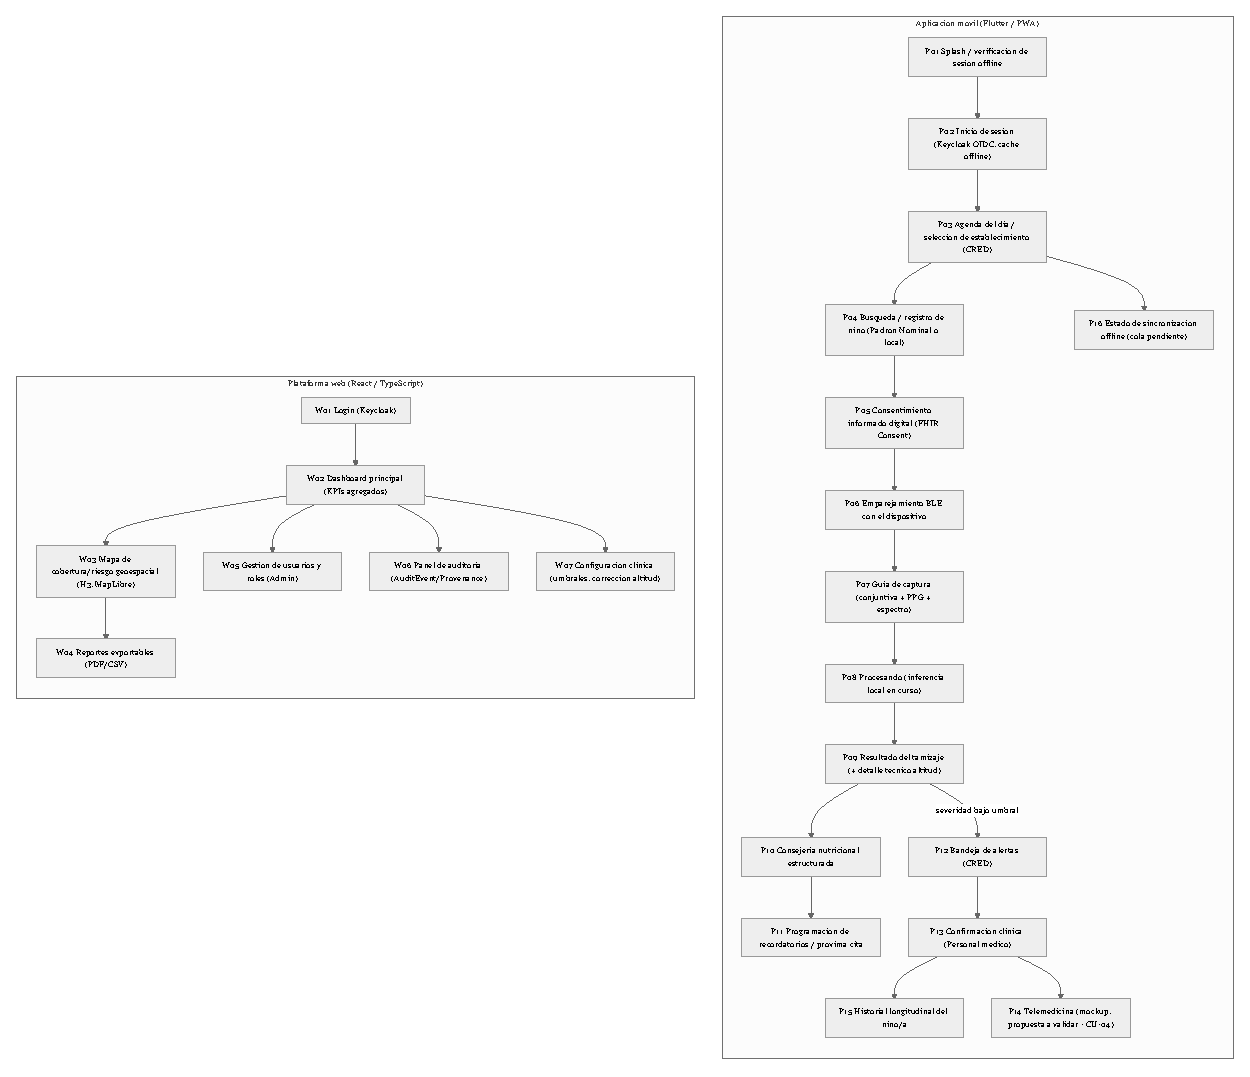
\includegraphics[width=0.98\linewidth,height=0.86\textheight,keepaspectratio]{assets/05-requerimientos/diagrama-01-sitemap.pdf}
\end{figure}

\subsection{2.3 Pantallas principales --- Aplicación móvil}\label{pantallas-principales-aplicaciuxf3n-muxf3vil}

Se presentan como mockups renderizados las ocho pantallas de mayor criticidad funcional y normativa (P02, P03, P05, P06, P07, P09, P12, P13); las ocho restantes se describen en la tabla resumen posterior a los wireframes.

\begin{figure}[H]
\centering
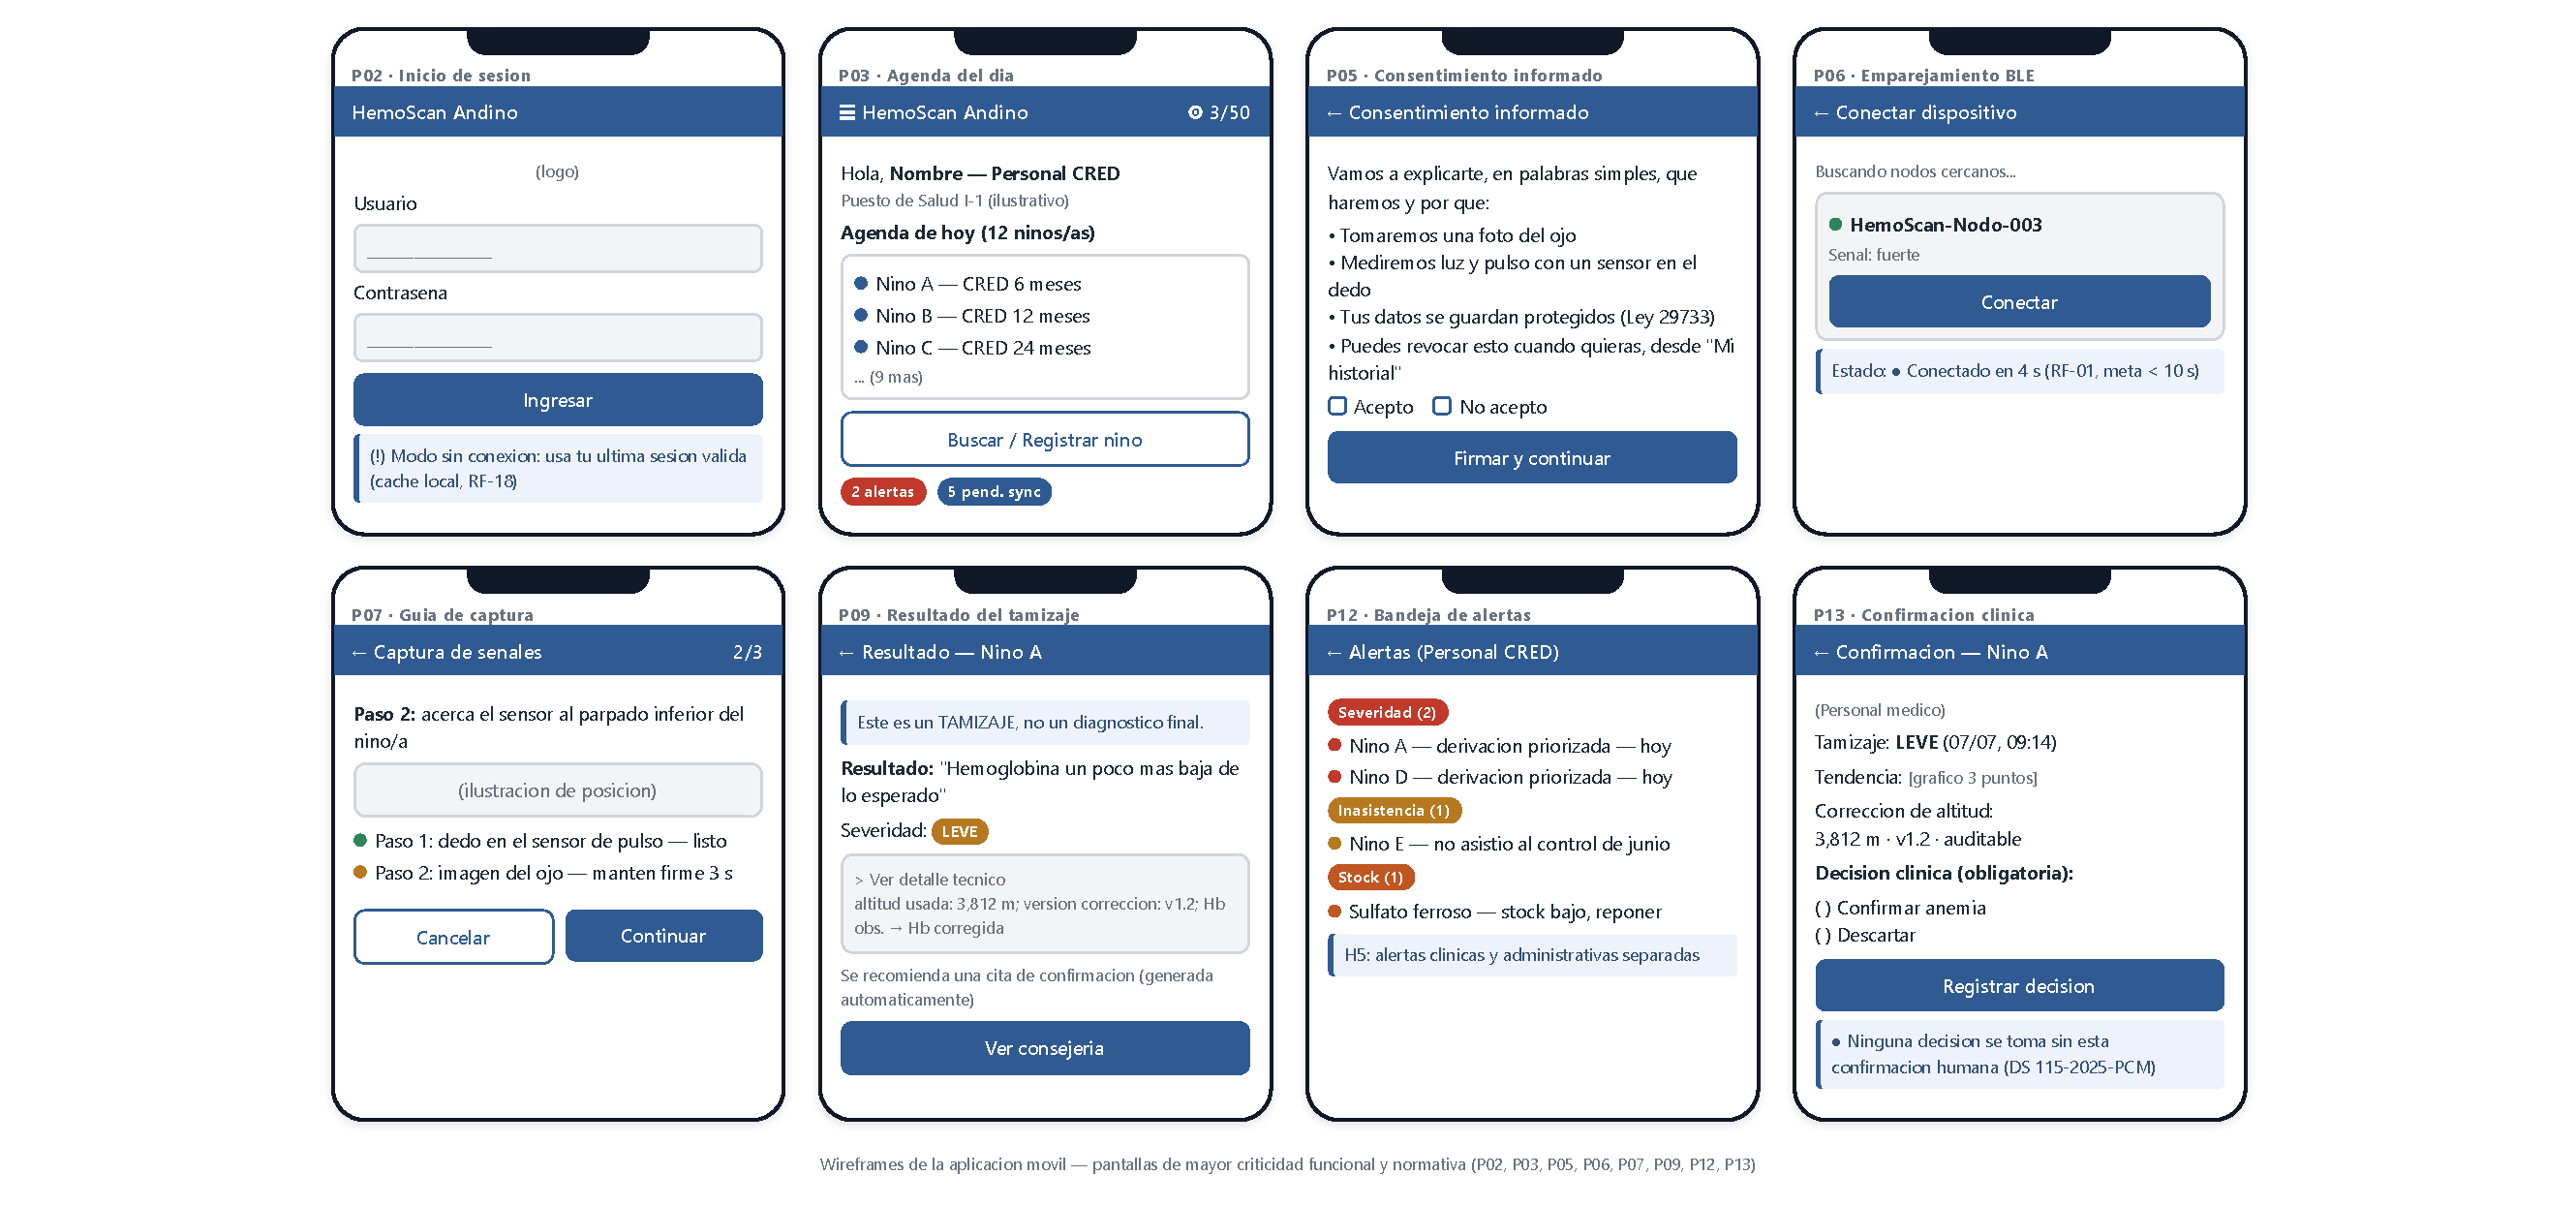
\includegraphics[width=1.0\linewidth,height=0.86\textheight,keepaspectratio]{assets/05-requerimientos/wireframes-movil.pdf}
\end{figure}

\textbf{Pantallas complementarias (descripción resumida):}

{\small
\begin{longtable}[]{@{}
  >{\raggedright\arraybackslash}p{(\linewidth - 4\tabcolsep) * \real{0.3333}}
  >{\raggedright\arraybackslash}p{(\linewidth - 4\tabcolsep) * \real{0.3333}}
  >{\raggedright\arraybackslash}p{(\linewidth - 4\tabcolsep) * \real{0.3333}}@{}}
\toprule\noalign{}
\begin{minipage}[b]{\linewidth}\raggedright
Pantalla
\end{minipage} & \begin{minipage}[b]{\linewidth}\raggedright
Rol principal
\end{minipage} & \begin{minipage}[b]{\linewidth}\raggedright
Contenido esencial
\end{minipage} \\
\midrule\noalign{}
\endhead
\bottomrule\noalign{}
\endlastfoot
P01 --- Splash / verificación de sesión offline & Todos & Logo, verificación de sesión en caché local, indicador de estado de batería/conexión del teléfono \\
P04 --- Búsqueda/registro de niño & Personal CRED & Buscador con consulta al Padrón Nominal (si hay conectividad) o formulario de registro local mínimo (si no la hay) \\
P08 --- Procesando & Personal CRED & Indicador de progreso de la inferencia local (\textless{} 3 s, RF-06) con retroalimentación háptica al finalizar (hallazgo H4, sección 2.5) \\
P10 --- Consejería nutricional & Cuidador/a, Personal CRED & Contenido estructurado del motor de reglas (RF-15), personalizado por edad/severidad, con opción de compartir por SMS/WhatsApp con el cuidador \\
P11 --- Programación de recordatorios & Cuidador/a & Confirmación de fecha del próximo control mensual y canal de recordatorio preferido (push o SMS) \\
P14 --- Telemedicina (mockup) & Personal médico & \emph{Mockup de baja fidelidad, marcado explícitamente ``Propuesta a validar --- no disponible en Fase 0''}; simula una videollamada con datos de tamizaje visibles en paralelo \\
P15 --- Historial longitudinal & Personal médico, Personal CRED & Gráfico de tendencia de hemoglobina corregida a lo largo de los controles (RF-20), con marcadores de eventos (derivación, confirmación, inicio de hierro) \\
P16 --- Estado de sincronización offline & Todos los roles de campo & Lista de registros pendientes de sincronizar, última sincronización exitosa, botón de sincronización manual forzada \\
\end{longtable}
}

\subsection{2.4 Pantallas principales --- Plataforma web}\label{pantallas-principales-plataforma-web}

\begin{figure}[H]
\centering
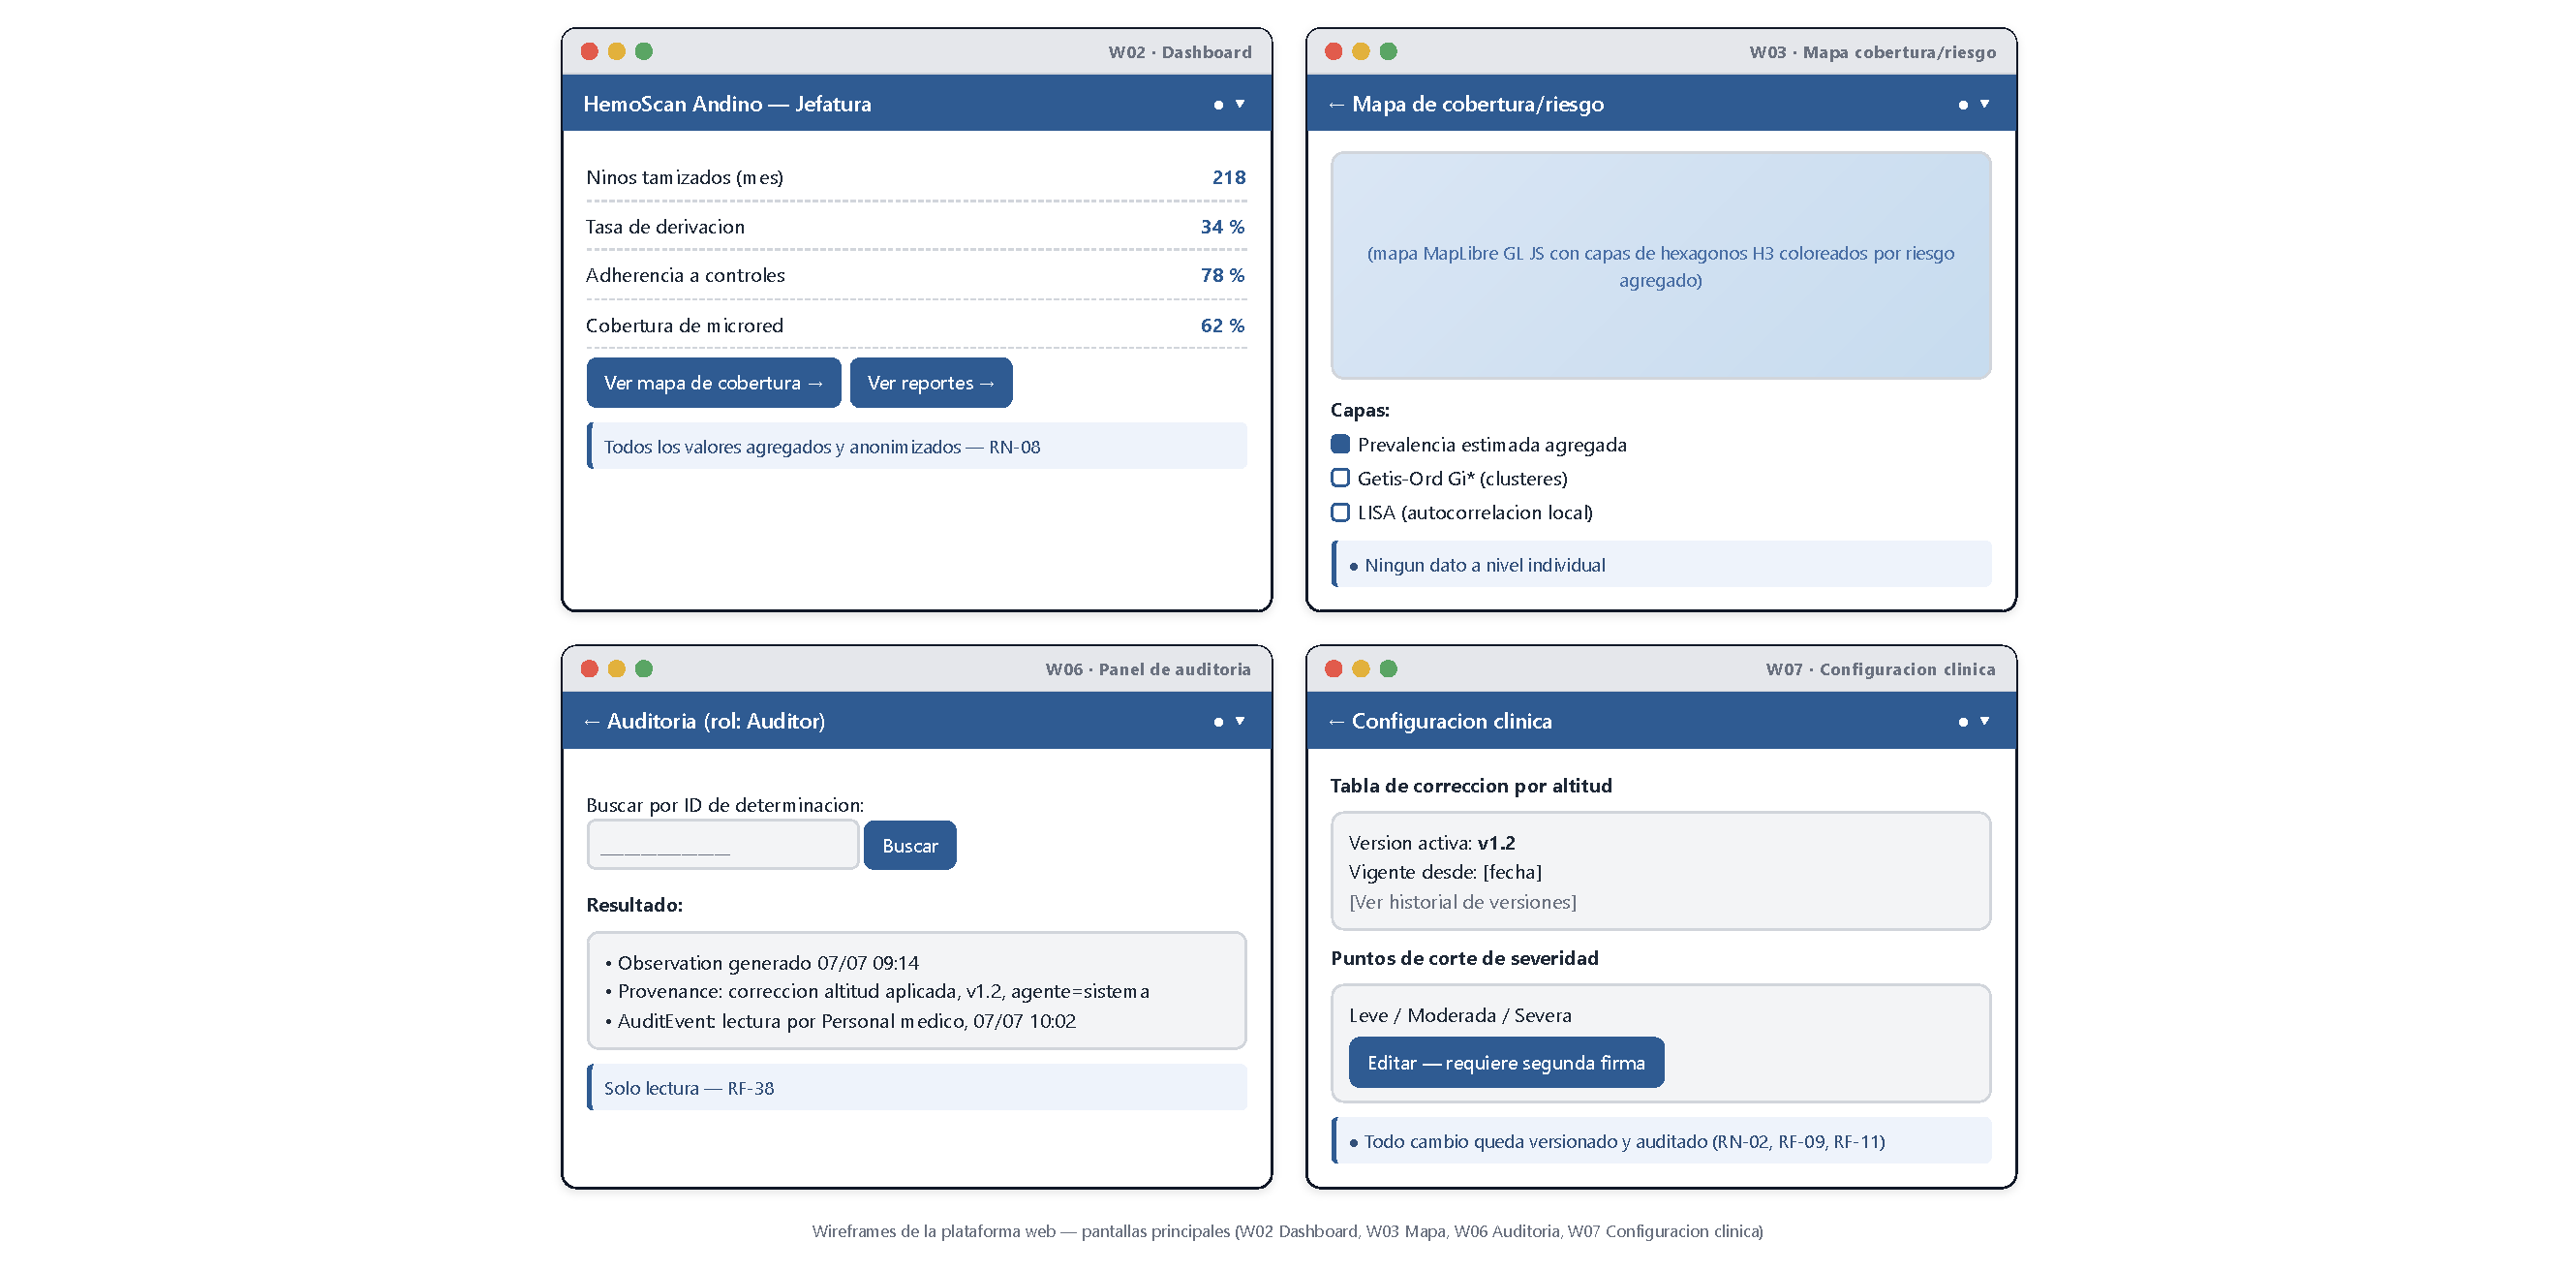
\includegraphics[width=0.92\linewidth,height=0.86\textheight,keepaspectratio]{assets/05-requerimientos/wireframes-web.pdf}
\end{figure}

\textbf{Pantallas complementarias (descripción resumida):}

{\small
\begin{longtable}[]{@{}
  >{\raggedright\arraybackslash}p{(\linewidth - 4\tabcolsep) * \real{0.3333}}
  >{\raggedright\arraybackslash}p{(\linewidth - 4\tabcolsep) * \real{0.3333}}
  >{\raggedright\arraybackslash}p{(\linewidth - 4\tabcolsep) * \real{0.3333}}@{}}
\toprule\noalign{}
\begin{minipage}[b]{\linewidth}\raggedright
Pantalla
\end{minipage} & \begin{minipage}[b]{\linewidth}\raggedright
Rol principal
\end{minipage} & \begin{minipage}[b]{\linewidth}\raggedright
Contenido esencial
\end{minipage} \\
\midrule\noalign{}
\endhead
\bottomrule\noalign{}
\endlastfoot
W01 --- Login & Todos los roles web & Redirección a Keycloak (OIDC); sin gestión de contraseñas propia (ADR-09) \\
W04 --- Reportes exportables & Jefatura, Analista DIRESA/GERESA & Tablas de throughput/adherencia/cobertura por establecimiento y periodo, con exportación PDF/CSV (RF-36) \\
W05 --- Gestión de usuarios y roles & Administrador & Alta/baja/modificación de usuarios, asignación de roles RBAC, historial de cambios (RF-37) \\
\end{longtable}
}

\subsection{2.5 Evidencia de validación con usuarios}\label{evidencia-de-validaciuxf3n-con-usuarios}

Dada la ausencia de convenio institucional real y, por tanto, de acceso a usuarios finales reales (personal CRED, personal médico o cuidadores/as de la Microred de Salud Altiplano-Puno), la validación de este prototipo se realizó mediante dos técnicas internas, cuya acta formal se presenta íntegra en el \textbf{Anexo C}: \textbf{(1)} una evaluación heurística interna aplicando una adaptación de las 10 heurísticas de usabilidad de Nielsen a las 23 pantallas del prototipo, ejecutada por los 3 integrantes del equipo; y \textbf{(2)} un recorrido cognitivo (\emph{cognitive walkthrough}) de los flujos CU-01, CU-02 y CU-03 con 3 personas voluntarias ajenas al equipo, actuando como \emph{proxies} de los perfiles ``Personal CRED'' y ``Cuidador/a'' --- se declara explícitamente que estas personas \textbf{no son personal de salud real ni cuidadores reales de la zona de intervención}, por lo que sus observaciones tienen valor exploratorio, no representativo.

De este ejercicio se identificaron y corrigieron siete hallazgos concretos, que se resumen en la siguiente tabla (el detalle completo de participantes, agenda y hallazgos consta en el Anexo C):

{\small
\begin{longtable}[]{@{}
  >{\raggedright\arraybackslash}p{(\linewidth - 6\tabcolsep) * \real{0.2500}}
  >{\raggedright\arraybackslash}p{(\linewidth - 6\tabcolsep) * \real{0.2500}}
  >{\raggedright\arraybackslash}p{(\linewidth - 6\tabcolsep) * \real{0.2500}}
  >{\raggedright\arraybackslash}p{(\linewidth - 6\tabcolsep) * \real{0.2500}}@{}}
\toprule\noalign{}
\begin{minipage}[b]{\linewidth}\raggedright
N.°
\end{minipage} & \begin{minipage}[b]{\linewidth}\raggedright
Hallazgo
\end{minipage} & \begin{minipage}[b]{\linewidth}\raggedright
Heurística/técnica que lo detectó
\end{minipage} & \begin{minipage}[b]{\linewidth}\raggedright
Cambio aplicado al prototipo
\end{minipage} \\
\midrule\noalign{}
\endhead
\bottomrule\noalign{}
\endlastfoot
H1 & El texto del resultado usaba el término médico ``anémico'' de forma directa & Lenguaje del usuario (Nielsen) & Se reemplazó por ``hemoglobina un poco más baja de lo esperado para tu edad'' (P09) \\
H2 & No era evidente que el consentimiento pudiera revocarse & Visibilidad del estado del sistema & Se agregó un botón explícito ``Revocar consentimiento'' en el historial (CU-02, flujo alterno A1) \\
H3 & El detalle técnico de la corrección por altitud saturaba la pantalla de resultado por defecto & Estética y diseño minimalista & Se convirtió en una sección colapsable ``Ver detalle técnico'' (P09) \\
H4 & Un participante no identificó cuándo el dispositivo había terminado de capturar & Visibilidad del estado del sistema & Se agregó un indicador de progreso explícito con retroalimentación háptica/sonora (P08) \\
H5 & La bandeja de alertas mezclaba severidad clínica con alertas administrativas de stock, generando confusión sobre prioridad & Reconocimiento antes que recuerdo & Se separaron en secciones con codificación de color e iconografía distinta (P12) \\
H6 & El flujo de emparejamiento BLE no explicaba qué hacer ante un fallo & Ayuda para reconocer y recuperarse de errores & Se agregó un mensaje de error con pasos de recuperación explícitos (P06) \\
H7 & Un participante confundió el ícono de ``sin conexión'' con un error del sistema & Coincidencia entre el sistema y el mundo real & Se agregó una etiqueta textual explícita junto al ícono (``Modo sin conexión --- tus datos se guardan localmente'') (P16) \\
\end{longtable}
}

Se declara explícitamente, en línea con el principio de honestidad metodológica del proyecto, que esta evidencia constituye una \textbf{validación interna/heurística de diseño}, útil para depurar errores gruesos de usabilidad antes de la construcción, pero \textbf{no equivale a una validación con stakeholders reales}. Esta limitación se retoma sin atenuantes en la autoevaluación final del documento.

\begin{center}\rule{0.5\linewidth}{0.5pt}\end{center}

\section{3. Diseño Arquitectónico}\label{diseuxf1o-arquitectuxf3nico}

\subsection{3.1 Estilo arquitectónico y vista general}\label{estilo-arquitectuxf3nico-y-vista-general}

HemoScan Andino adopta un estilo arquitectónico híbrido, deliberadamente ajustado a sus restricciones (sección 1.5) más que a una plantilla genérica: \textbf{offline-first en el cliente} (local-first, con sincronización diferida), \textbf{monolito modular en el backend} (no microservicios desde el inicio) y \textbf{procesamiento embebido en el borde} (edge inference) para el componente de inteligencia artificial. La siguiente vista general de alto nivel sitúa los cuatro subsistemas ya introducidos en la sección 1.1 y sus relaciones principales:

\textbf{Diagrama 2 --- Vista general de arquitectura (componentes de alto nivel).}

\begin{figure}[H]
\centering
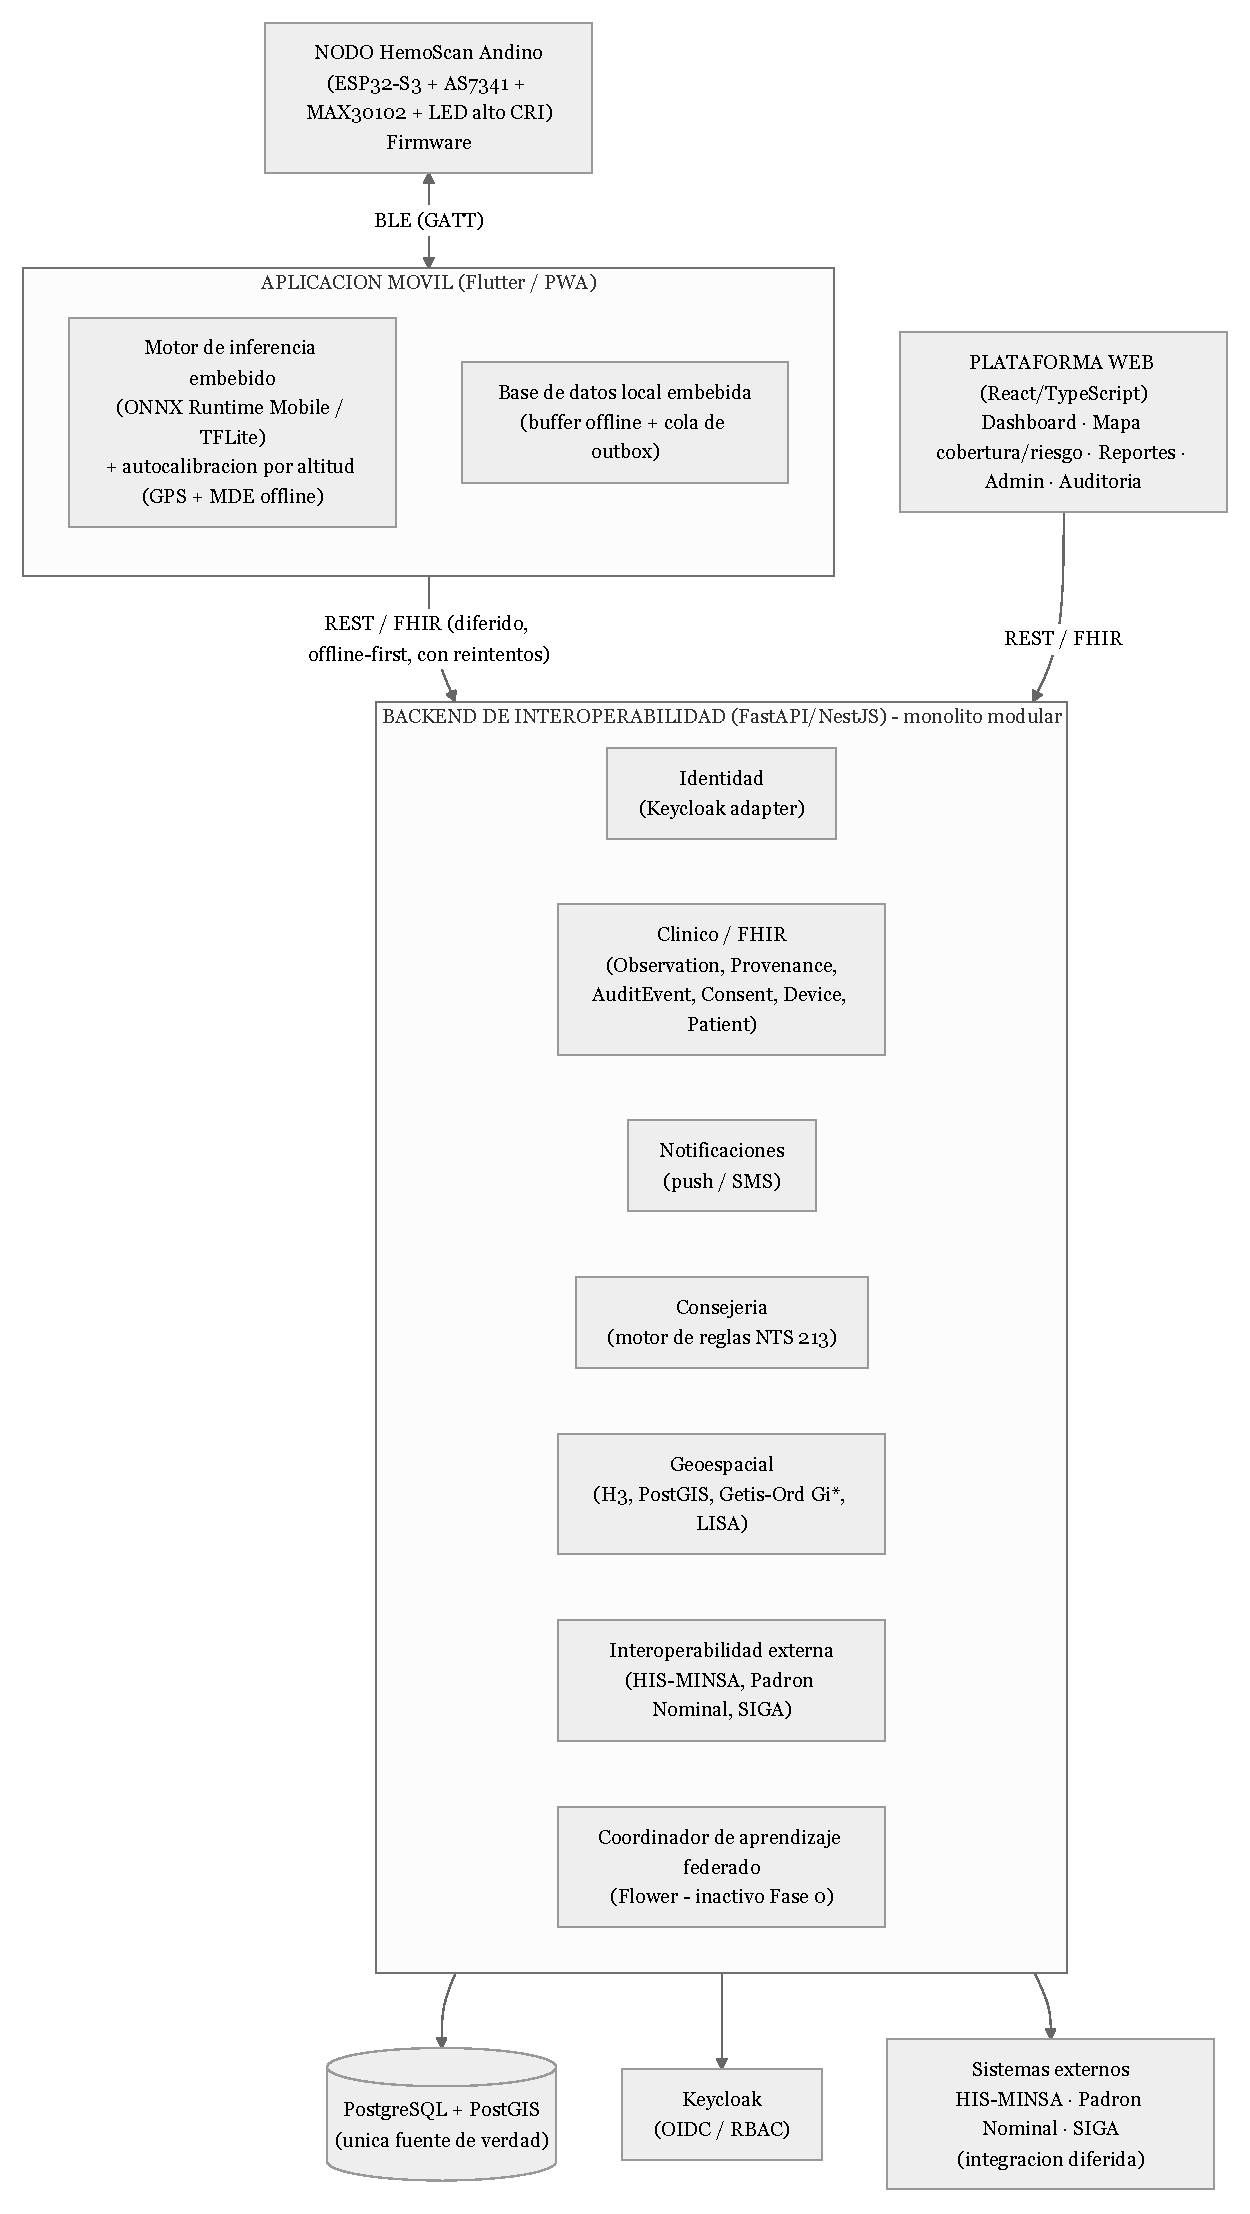
\includegraphics[width=0.9\linewidth,height=0.86\textheight,keepaspectratio]{assets/05-requerimientos/diagrama-02-arquitectura-alto-nivel.pdf}
\end{figure}

\subsection{3.2 Diagrama de componentes}\label{diagrama-de-componentes}

\textbf{Diagrama 3 --- Diagrama de componentes (notación UML textual).} Leyenda: \texttt{{[}C{]}} componente; \texttt{o} interfaz proveída (\emph{provided interface}); \texttt{)} interfaz requerida (\emph{required interface}); \texttt{-\/-\/-\textgreater{}} dependencia/uso.

\begin{figure}[H]
\centering
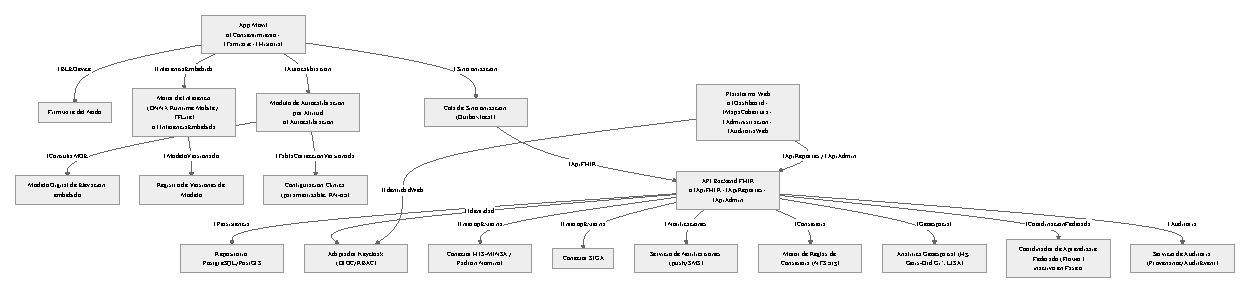
\includegraphics[width=0.98\linewidth,height=0.86\textheight,keepaspectratio]{assets/05-requerimientos/diagrama-03-componentes.pdf}
\end{figure}

Este diagrama de componentes hace explícita una decisión de diseño central: el \textbf{Módulo de Autocalibración por Altitud} y el \textbf{Motor de Inferencia} son componentes desacoplados entre sí (ADR-05, sección 3.5), de modo que un cambio futuro en la fórmula de corrección de altitud no requiere modificar ni reentrenar el modelo de inferencia de hemoglobina. De igual manera, el \textbf{Coordinador de Aprendizaje Federado} existe como componente desde Fase 0, pero permanece inactivo (ADR-08), evitando así deuda técnica de una futura reintroducción sin dejar de cumplir, hoy, con el alcance real del piloto.

\subsection{3.3 Diagrama de despliegue}\label{diagrama-de-despliegue}

\textbf{Diagrama 4 --- Diagrama de despliegue.} Leyenda: \texttt{«nodo»} nodo físico/lógico de despliegue; \texttt{«artefacto»} software desplegado en el nodo; \texttt{-\textgreater{}} protocolo de comunicación entre nodos.

\begin{figure}[H]
\centering
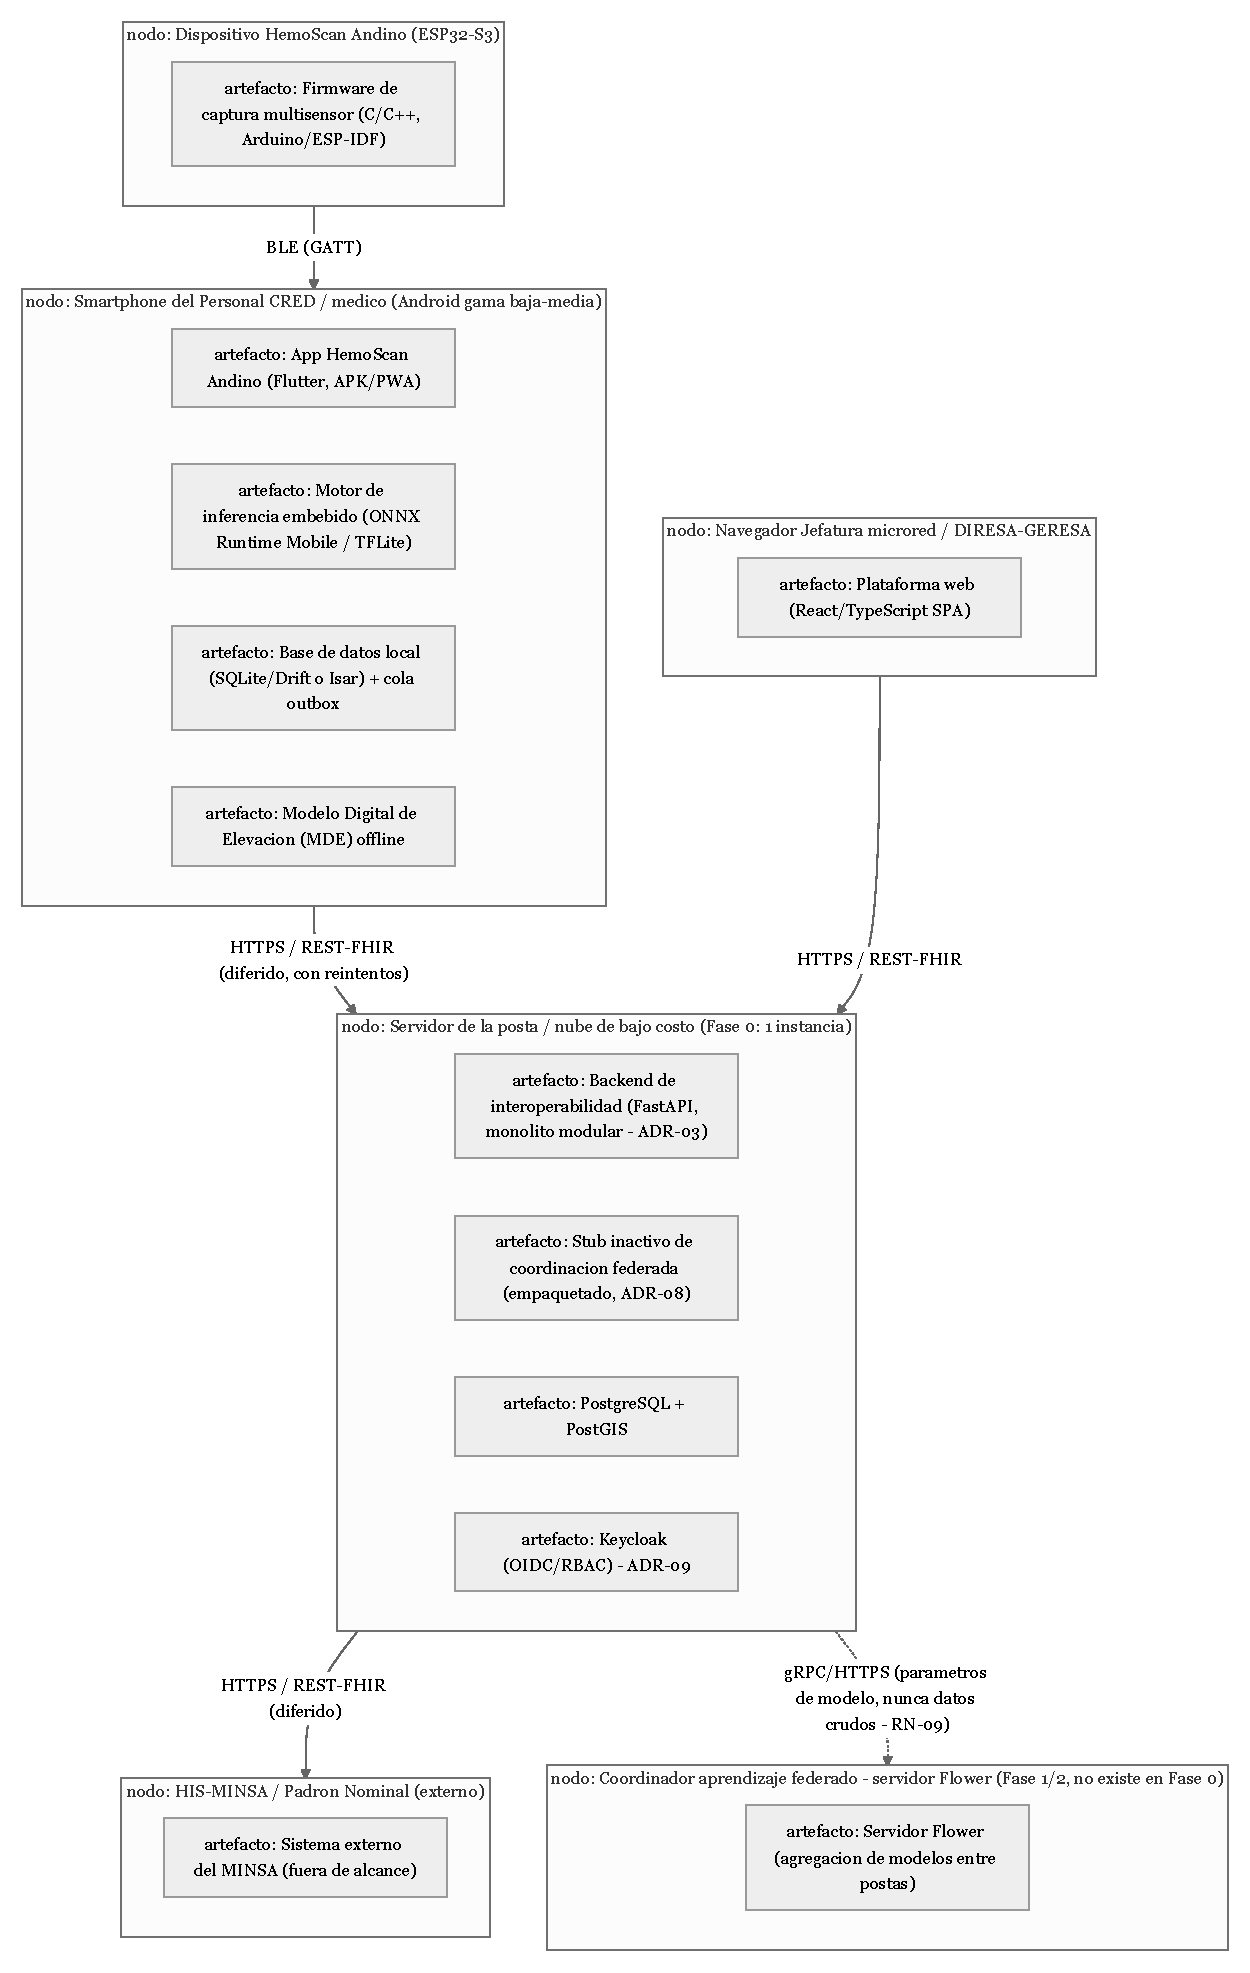
\includegraphics[width=0.92\linewidth,height=0.86\textheight,keepaspectratio]{assets/05-requerimientos/diagrama-04-despliegue.pdf}
\end{figure}

El diagrama refleja deliberadamente que, en Fase 0, existe \textbf{un único servidor} (posta o nube de bajo costo) alojando el backend ---incluido el stub inactivo de coordinación federada, empaquetado como artefacto desde Fase 0---, la base de datos y Keycloak ---consistente con el presupuesto de S/ 320 para 8 meses ya comprometido (Entregable N.° 2)---, y que el \textbf{nodo físico dedicado} de coordinación de aprendizaje federado (un servidor Flower independiente) se documenta como extensión futura pero no se despliega, en coherencia con la ADR-08 (ver su aclaración de consistencia entre diagramas). La validación de la capacidad real de este servidor único (CPU, memoria, ancho de banda) para sostener simultáneamente estos artefactos es una responsabilidad explícita del Integrante 1 (Infraestructura Tecnológica, paquete EDT 2.2), no de este entregable.

\subsection{3.4 Mapeo de requerimientos no funcionales a tácticas arquitectónicas}\label{mapeo-de-requerimientos-no-funcionales-a-tuxe1cticas-arquitectuxf3nicas}

{\small
\begin{longtable}[]{@{}
  >{\raggedright\arraybackslash}p{(\linewidth - 4\tabcolsep) * \real{0.3333}}
  >{\raggedright\arraybackslash}p{(\linewidth - 4\tabcolsep) * \real{0.3333}}
  >{\raggedright\arraybackslash}p{(\linewidth - 4\tabcolsep) * \real{0.3333}}@{}}
\toprule\noalign{}
\begin{minipage}[b]{\linewidth}\raggedright
RNF
\end{minipage} & \begin{minipage}[b]{\linewidth}\raggedright
Táctica arquitectónica aplicada
\end{minipage} & \begin{minipage}[b]{\linewidth}\raggedright
Componente(s) responsable(s)
\end{minipage} \\
\midrule\noalign{}
\endhead
\bottomrule\noalign{}
\endlastfoot
RNF-01, RNF-02 (desempeño) & Inferencia embebida en el dispositivo (sin \emph{round-trip} de red); modelo optimizado para móvil & Motor de Inferencia \\
RNF-03, RNF-04, RNF-17 (disponibilidad offline) & Patrón \emph{local-first} + \emph{outbox}; base de datos embebida como fuente de verdad del cliente & App Móvil, Cola de Sincronización \\
RNF-05, RNF-06, RNF-07, RNF-19 (seguridad y privacidad) & TLS de extremo a extremo; cifrado en reposo; identidad delegada a Keycloak; agregación/anonimización antes de exponer datos geoespaciales & Adaptador Keycloak, Repositorio PostgreSQL, Servicio de Analítica Geoespacial \\
RNF-08, RNF-18 (trazabilidad/auditabilidad de IA) & Generación obligatoria de Provenance/AuditEvent en cada operación clínica o de inferencia; versionado de modelo y de tabla de corrección & Servicio de Auditoría, Módulo de Autocalibración, Motor de Inferencia \\
RNF-09 (supervisión humana) & Ninguna transición de estado crítica (confirmación, prescripción) ocurre sin una acción de usuario autenticado con rol habilitado & API Backend FHIR (validación de reglas de negocio en el servidor, no solo en el cliente) \\
RNF-10 (interoperabilidad) & Adopción estricta del estándar HL7 FHIR para el modelo de datos clínico & Conector HIS-MINSA/Padrón Nominal, API Backend FHIR \\
RNF-12, RNF-13 (escalabilidad y mantenibilidad) & Monolito modular con límites de dominio explícitos, preparado para una futura extracción a microservicios (ADR-02) & Backend de Interoperabilidad (todos los módulos) \\
RNF-14, RNF-15 (usabilidad y accesibilidad) & Validación heurística iterativa (sección 2.5); localización parametrizable de textos & App Móvil \\
RNF-16 (eficiencia energética) & Fuera del control directo del software; se traslada como restricción de diseño de firmware/hardware & Firmware del Nodo (responsabilidad compartida con Infraestructura Tecnológica) \\
RNF-20 (disponibilidad del backend) & Responsabilidad de infraestructura de despliegue (fuera del alcance de este entregable) & Servidor de la posta / nube (Integrante 1) \\
\end{longtable}
}

\subsection{3.5 Registro de decisiones arquitectónicas (ADR)}\label{registro-de-decisiones-arquitectuxf3nicas-adr}

Se documentan diez decisiones arquitectónicas en formato estándar (Contexto, Decisión, Consecuencias, Alternativas consideradas), incluyendo explícitamente aquellas que el enunciado original del proyecto dejó abiertas como disyuntiva (FastAPI/NestJS, ONNX/TFLite) y las que surgen directamente del encargo de factibilidad del Entregable N.° 4 (telemedicina, aprendizaje federado).

\textbf{ADR-01 --- Arquitectura offline-first con sincronización diferida (patrón local-first + outbox)}
- \emph{Estado:} Aceptada.
- \emph{Contexto:} conectividad intermitente o nula en la zona rural altoandina de la microred ilustrativa (Entregables N.° 1 y N.° 4, escenario ``sin cobertura'').
- \emph{Decisión:} la base de datos embebida del dispositivo/app es la fuente de verdad del cliente; toda escritura se encola localmente (patrón \emph{outbox}) y se reintenta automáticamente al detectar conectividad; el backend acepta \emph{bundles} FHIR idempotentes, identificados por un UUID generado en el cliente, para evitar duplicados ante reintentos.
- \emph{Consecuencias:} (+) cumple RF-18/RNF-03; (+) resiliente a redes inestables; (--) mayor complejidad de resolución de conflictos e idempotencia; (--) el cliente debe validar localmente reglas de negocio que en un sistema \emph{thin-client} solo existirían en el servidor.
- \emph{Alternativas consideradas:} cliente \emph{thin} dependiente de conectividad permanente (rechazada: incompatible con el contexto rural); cola de mensajería dedicada tipo Kafka/RabbitMQ desde Fase 0 (rechazada por sobre-ingeniería para 150-300 casos; a reevaluar en Fase 2).

\textbf{ADR-02 --- Monolito modular como estilo de backend (no microservicios desde el inicio)}
- \emph{Estado:} Aceptada.
- \emph{Contexto:} un desarrollador principal (Integrante 3) con apoyo puntual; presupuesto de S/ 320 para servidor/nube en 8 meses; volumen inicial de 150-300 niños en 1 microred.
- \emph{Decisión:} backend organizado como monolito modular, con módulos de dominio delimitados (identidad, clínico/FHIR, notificaciones, consejería, geoespacial, interoperabilidad, coordinación federada), cada uno con límites claros que faciliten una futura extracción a microservicios si el volumen de Fase 2 lo justifica.
- \emph{Consecuencias:} (+) menor costo operativo y de coordinación; (+) despliegue simple en un único servidor de bajo costo; (--) menor aislamiento de fallos entre módulos que en microservicios; (--) exige disciplina de diseño para no degenerar en un monolito no modular (tablas acopladas entre dominios).
- \emph{Alternativas consideradas:} microservicios desde Fase 0 (rechazada: sobre-ingeniería para el volumen y equipo disponibles); arquitectura serverless/FaaS (rechazada por la necesidad de procesos de larga duración, como el coordinador de aprendizaje federado y la analítica espacial por lotes).

\textbf{ADR-03 --- Elección tentativa de FastAPI (Python) como framework de backend para Fase 0}
- \emph{Estado:} Propuesta, decisión reversible (no definitiva).
- \emph{Contexto:} el enunciado del proyecto deja abierta la disyuntiva ``FastAPI o NestJS''; el equipo ya usa Python para el motor de inferencia, la analítica espacial (PySAL/esda) y el coordinador de aprendizaje federado (Flower, nativo en Python).
- \emph{Decisión:} adoptar FastAPI como framework tentativo de Fase 0, compartiendo lenguaje y entorno de ejecución con el resto del stack analítico, sin requerir un segundo runtime (Node.js) exclusivamente para el backend.
- \emph{Consecuencias:} (+) un solo lenguaje de backend/analítica/inferencia reduce la curva de aprendizaje de un equipo de 3 personas; (+) FastAPI ofrece tipado con Pydantic, de ergonomía cercana a los DTOs de NestJS; (--) se renuncia, por ahora, al ecosistema de inyección de dependencias más maduro de NestJS y a la afinidad de lenguaje con un frontend TypeScript/React; (--) esta decisión no ha sido validada aún por el Integrante 1 en cuanto a su impacto en el despliegue.
- \emph{Alternativas consideradas:} NestJS (Node/TypeScript) --- descartada solo tentativamente por la sinergia de lenguaje único con el stack analítico Python, no por una deficiencia técnica propia. \textbf{Se marca explícitamente como reversible}: de incorporarse al equipo mayor dominio de Node.js/NestJS antes del inicio de la construcción (Mes 5), debe reabrirse mediante el procedimiento de control de cambios (Entregable N.° 3, sección 3.2.4).

\textbf{ADR-04 --- ONNX Runtime Mobile como motor de inferencia primario, con ruta alterna a TFLite}
- \emph{Estado:} Aceptada.
- \emph{Contexto:} el enunciado especifica ``ONNX/TFLite'' como opciones de inferencia embebida.
- \emph{Decisión:} entrenar el modelo multimodal en un formato canónico y exportarlo a ONNX; ejecutar la inferencia mediante ONNX Runtime Mobile como ruta primaria (evita una conversión adicional con pérdida hacia TFLite); mantener la exportación a TFLite como ruta de contingencia para dispositivos Android de gama muy baja sin soporte adecuado de ONNX Runtime Mobile.
- \emph{Consecuencias:} (+) una sola fuente de verdad del modelo (ONNX) con dos rutas de despliegue; (--) requiere validar en banco de pruebas (historias HC05/HC06, Entregable N.° 3) el rendimiento real de ambos \emph{runtimes} en el hardware de referencia antes de fijar la ruta definitiva, dado que el modelo exacto de smartphone de referencia es \textbf{{[}DATO PENDIENTE DE VALIDAR{]}}.
- \emph{Alternativas consideradas:} usar exclusivamente TFLite (rechazada por ahora: exigiría una conversión adicional desde el formato de entrenamiento, con riesgo de pérdida de precisión no cuantificada).

\textbf{ADR-05 --- Autocalibración por altitud como módulo independiente y auditable}
- \emph{Estado:} Aceptada (mandato explícito del proyecto; ver RN-02, RN-03).
- \emph{Contexto:} el riesgo de sobrediagnóstico por corrección inadecuada de hemoglobina en altitud (Gonzales et al.~2025; Baquerizo-Sedano et al.~2025) exige que la corrección sea auditable y nunca basada en altitud cruda de GPS.
- \emph{Decisión:} implementar la corrección por altitud como un componente desacoplado del motor de inferencia de hemoglobina, con fuente de datos propia (MDE embebido), versión propia y registro auditable propio (Provenance).
- \emph{Consecuencias:} (+) un cambio futuro en la fórmula de corrección ---por ejemplo, ante nueva evidencia científica--- no requiere modificar ni reentrenar el modelo de inferencia; (+) auditable de forma independiente; (--) introduce una dependencia adicional (el MDE embebido) que debe empaquetarse y actualizarse junto con la app.
- \emph{Alternativas consideradas:} incorporar la corrección como parte interna e inseparable del modelo de inferencia (rechazada: acoplaría dos fuentes de incertidumbre distintas ---el modelo óptico y la corrección geográfica--- dificultando la auditoría independiente de cada una).

\textbf{ADR-06 --- Alcance de recursos FHIR fijo en 6 tipos para Fase 0; MedicationRequest diferido}
- \emph{Estado:} Aceptada para Fase 0 / a reevaluar en Fase 1.
- \emph{Contexto:} encargo explícito de factibilidad del Entregable N.° 4 (sección 1.9(b) de este documento).
- \emph{Decisión:} mantener Observation, Provenance, AuditEvent, Consent, Device y Patient como alcance validado; representar la prescripción de hierro como anotación estructurada de Observation en Fase 0; incorporar MedicationRequest solo cuando se validen (i) la posología exacta de la NTS 213-MINSA/DGIESP-2024 y (ii) la capacidad de ingesta del HIS-MINSA real.
- \emph{Consecuencias:} (+) no bloquea la Fase 0 por falta de un dato externo pendiente; (--) la anotación estructurada es menos expresiva que un recurso dedicado para reportes de adherencia a la posología.

\textbf{ADR-07 --- Telemedicina como extensión arquitectónica opcional, no incluida en el MVP de Fase 0}
- \emph{Estado:} Diferida a Fase 1.
- \emph{Contexto:} encargo explícito de factibilidad del Entregable N.° 4 (sección 1.9(a) de este documento).
- \emph{Decisión:} diseñar el módulo de Confirmación con un punto de extensión (interfaz \texttt{IConsultaRemota}) que permita anexar en el futuro un proveedor de videollamada/mensajería asíncrona, sin implementarlo ni depender de él en Fase 0.
- \emph{Consecuencias:} (+) no compromete el MVP a una dependencia de conectividad que contradice el diseño offline-first; (+) queda lista la interfaz para una incorporación futura sin rediseño; (--) la etapa de Confirmación sigue dependiendo del traslado físico en zonas sin telemedicina, tal como en el proceso AS-IS.
- \emph{Alternativas consideradas:} construir un MVP básico de videollamada en Fase 0 (rechazada: contradice el escenario ``sin cobertura'' documentado para gran parte del territorio, Entregable N.° 4, sección 4.3.1).

\textbf{ADR-08 --- Aprendizaje federado (Flower): presente en la arquitectura, no activado hasta Fase 1/2}
- \emph{Estado:} Aceptada (diseño presente, activación diferida).
- \emph{Contexto:} Fase 0 opera con una sola microred/nodo agregador; el aprendizaje federado solo aporta valor genuino con múltiples postas aportando actualizaciones de modelo de forma distribuida.
- \emph{Decisión:} exponer el módulo/interfaz de coordinación de aprendizaje federado desde Fase 0 (evitando deuda técnica de introducirlo después), pero no activar un ciclo real de reentrenamiento federado hasta que existan múltiples postas activas (Fase 2, escalamiento regional), coherente con el modelo de negocio de 3 fases del Business Case (Entregable N.° 2).
- \emph{Consecuencias:} (+) evita rediseño posterior; (--) no habrá evidencia empírica de mejora por reentrenamiento federado hasta la Fase 2.
- \emph{Aclaración de consistencia entre diagramas (añadida en esta revisión).} Una verificación interna detectó una ambigüedad entre el Diagrama 2/Diagrama 3 (que muestran el Coordinador de Aprendizaje Federado como un componente ya interno del backend, solo inactivo) y el Diagrama 4 (que lo muestra como un «nodo» físico separado ``no desplegado en Fase 0''). Se aclara explícitamente: el artefacto que se empaqueta con el backend \textbf{desde Fase 0} es únicamente la \textbf{interfaz/stub de coordinación} (\texttt{ICoordinacionFederada}, Diagrama 3) y su lógica mínima de agregación de parámetros, residiendo \textbf{inactiva dentro del mismo proceso/nodo del backend monolito} (el servidor único de la posta, Diagrama 4). Ningún servidor Flower dedicado ni proceso de coordinación distribuido se despliega como \textbf{nodo físico independiente} hasta la Fase 1/2, momento en el que ---si el volumen de postas lo justifica--- dicho módulo podría extraerse a un nodo propio, de forma consistente con la estrategia de extracción a microservicios ya prevista en ADR-02. El Diagrama 4 (sección 3.3) se actualiza en esta revisión para reflejar ambas realidades sin ambigüedad: (a) el nodo del servidor de la posta en Fase 0, que ya incluye el artefacto stub inactivo del coordinador; y (b) el nodo lógico ``Coordinador de aprendizaje federado (Fase 1/2)'', que representa la futura extracción a un servidor Flower dedicado y que, en efecto, no existe como artefacto desplegado independiente durante Fase 0.

\textbf{ADR-09 --- Identidad y control de acceso centralizados en Keycloak (OIDC/RBAC)}
- \emph{Estado:} Aceptada.
- \emph{Contexto:} necesidad de RBAC robusto (RF-37) sin invertir esfuerzo de desarrollo propio en gestión de credenciales, dada la sensibilidad de los datos (Ley N.° 29733).
- \emph{Decisión:} delegar la autenticación/autorización completamente a Keycloak; la aplicación y el backend nunca almacenan contraseñas propias.
- \emph{Consecuencias:} (+) reduce la superficie de riesgo de seguridad propia; (+) facilita RBAC estándar; (--) introduce una dependencia operativa de disponibilidad de Keycloak, que debe desplegarse con disponibilidad razonable incluso en el servidor de bajo costo de Fase 0 (responsabilidad trasladada al Integrante 1, paquete EDT 2.3).

\textbf{ADR-10 --- PostgreSQL + PostGIS como único motor de base de datos}
- \emph{Estado:} Aceptada.
- \emph{Contexto:} necesidad de soportar datos clínicos transaccionales y datos geoespaciales agregados (H3) con presupuesto y equipo reducidos.
- \emph{Decisión:} usar una única instancia de PostgreSQL con la extensión PostGIS para ambos tipos de datos, en lugar de una base de datos geoespacial separada.
- \emph{Consecuencias:} (+) simplifica la operación para el volumen y presupuesto de Fase 0; (+) PostGIS soporta directamente índices espaciales y agregación por hexágono H3; (--) a partir de cierto volumen (Fase 2), podría requerirse un almacén de datos analítico separado para no sobrecargar la base transaccional --- riesgo anotado para revisión futura por Infraestructura Tecnológica.

\begin{center}\rule{0.5\linewidth}{0.5pt}\end{center}

\section{4. Diseño Detallado}\label{diseuxf1o-detallado}

\subsection{4.1 Diagrama de casos de uso (UML)}\label{diagrama-de-casos-de-uso-uml}

\textbf{Diagrama 5 --- Diagrama de casos de uso.} \emph{(Renderizado a imagen vectorial desde una especificación en notación de diagrama-como-código, con un renderizador libre de licencia.)} Notación: \texttt{actor} (rol humano o sistema externo); \texttt{usecase} (caso de uso); \texttt{-\/-\textgreater{}} asociación actor-caso de uso; \texttt{..\textgreater{}} con etiqueta \texttt{\textless{}\textless{}include\textgreater{}\textgreater{}}/\texttt{\textless{}\textless{}extend\textgreater{}\textgreater{}} para inclusión obligatoria/extensión condicional; \texttt{\textless{}\textbar{}-\/-} generalización de actor.

\begin{figure}[H]
\centering
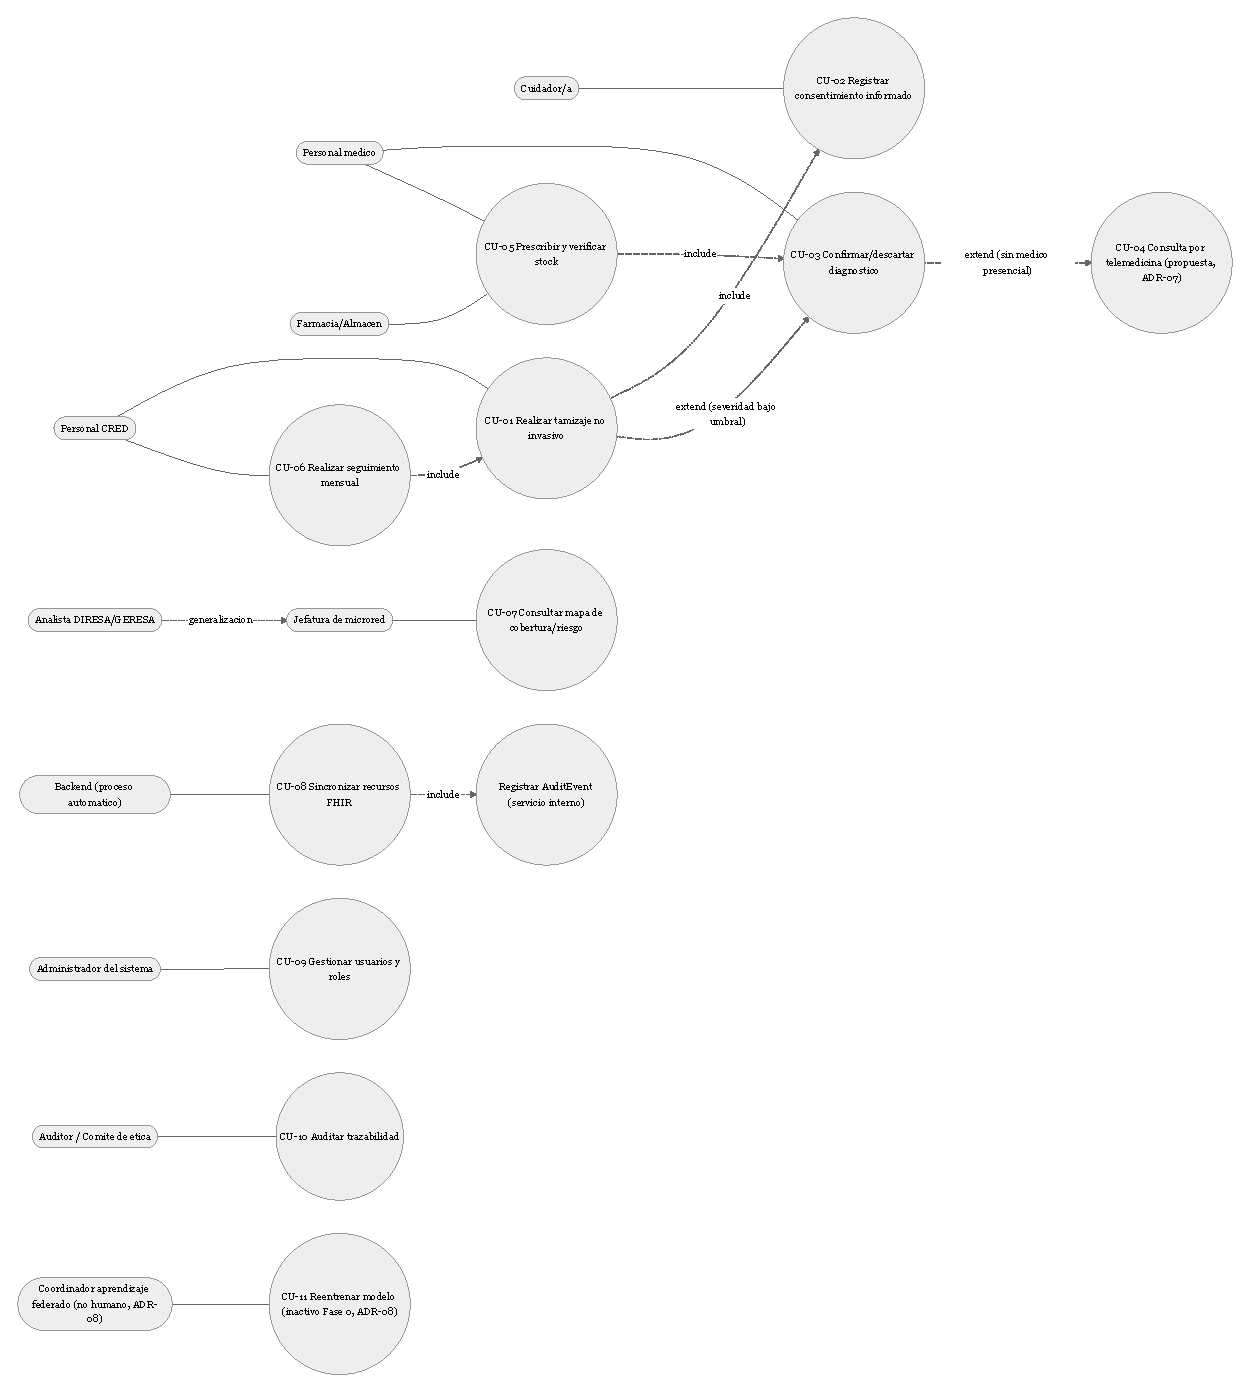
\includegraphics[width=1.0\linewidth,height=0.86\textheight,keepaspectratio]{assets/05-requerimientos/diagrama-05-casos-de-uso.pdf}
\end{figure}

\subsection{4.2 Diagrama de clases (UML)}\label{diagrama-de-clases-uml}

\textbf{Diagrama 6 --- Diagrama de clases del dominio.} \emph{(Renderizado a imagen vectorial desde una especificación \texttt{classDiagram} de diagrama-como-código, con un renderizador libre de licencia.)} Se desarrolla el núcleo de 12 clases centrales del dominio clínico y de trazabilidad, más las 8 clases complementarias de soporte administrativo y geoespacial (antes solo en la tabla posterior), ahora integradas en el mismo diagrama para que las multiplicidades sean sintácticamente verificables en un único modelo.

\begin{figure}[H]
\centering
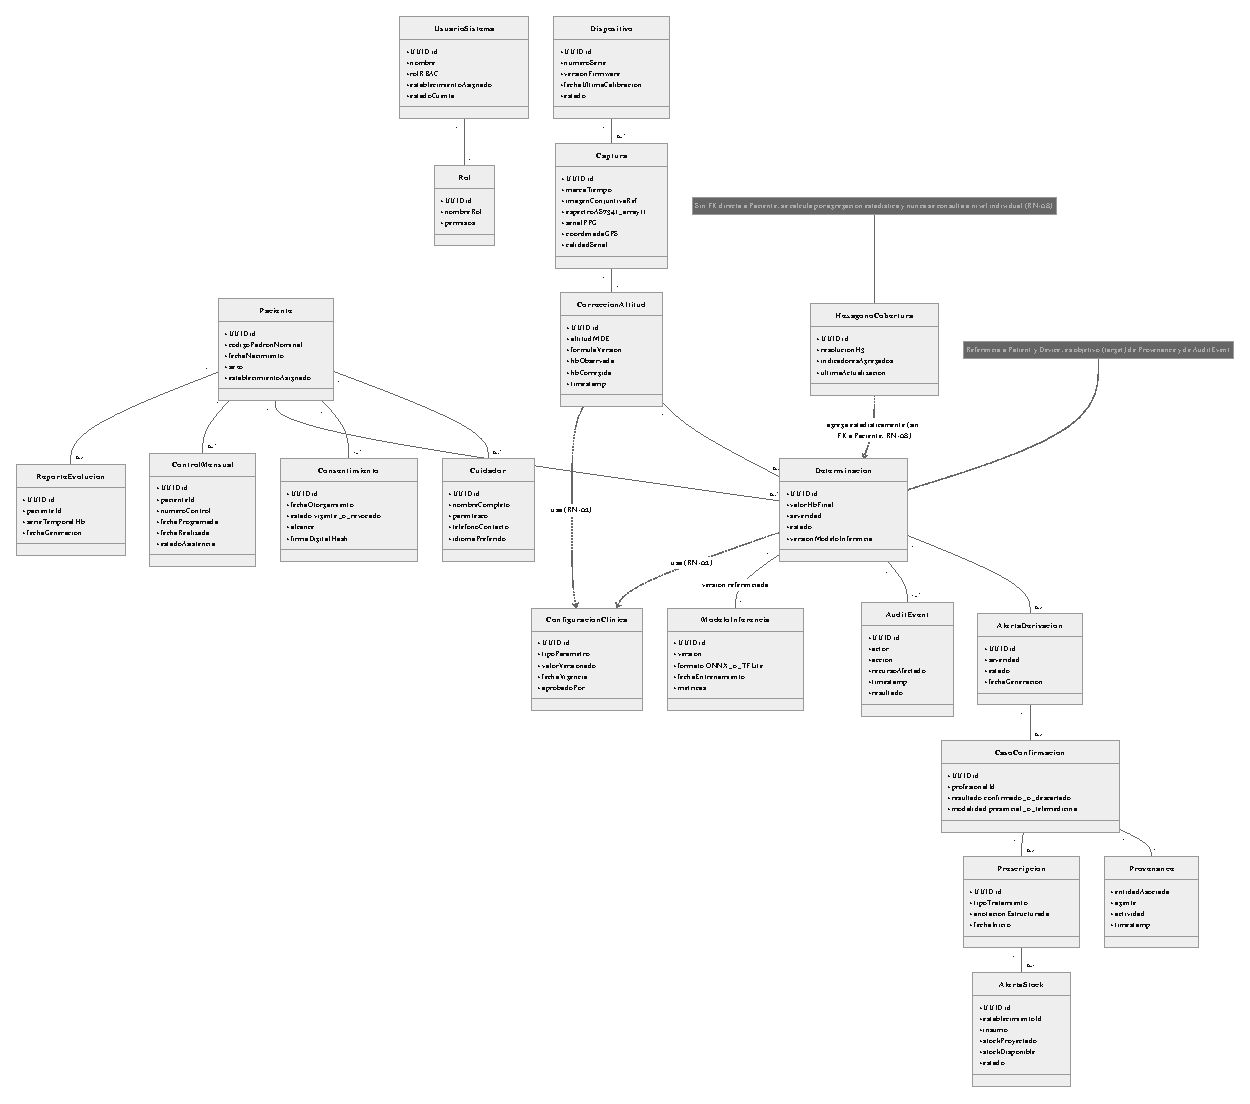
\includegraphics[width=1.0\linewidth,height=0.86\textheight,keepaspectratio]{assets/05-requerimientos/diagrama-06-clases-dominio.pdf}
\end{figure}

\textbf{Clases complementarias (soporte administrativo y geoespacial) --- tabla de referencia detallada.} \emph{(Estas 8 clases ya están integradas, con sus asociaciones y multiplicidades, en la sintaxis PlantUML del Diagrama 6; la tabla siguiente se conserva como referencia de lectura rápida de atributos y mapeo FHIR, sin duplicar información normativa nueva.)}

{\small
\begin{longtable}[]{@{}
  >{\raggedright\arraybackslash}p{(\linewidth - 6\tabcolsep) * \real{0.2500}}
  >{\raggedright\arraybackslash}p{(\linewidth - 6\tabcolsep) * \real{0.2500}}
  >{\raggedright\arraybackslash}p{(\linewidth - 6\tabcolsep) * \real{0.2500}}
  >{\raggedright\arraybackslash}p{(\linewidth - 6\tabcolsep) * \real{0.2500}}@{}}
\toprule\noalign{}
\begin{minipage}[b]{\linewidth}\raggedright
Clase
\end{minipage} & \begin{minipage}[b]{\linewidth}\raggedright
Atributos clave
\end{minipage} & \begin{minipage}[b]{\linewidth}\raggedright
Relación principal
\end{minipage} & \begin{minipage}[b]{\linewidth}\raggedright
Mapeo FHIR / notas
\end{minipage} \\
\midrule\noalign{}
\endhead
\bottomrule\noalign{}
\endlastfoot
ModeloInferencia & id, version, formato (ONNX/TFLite), fechaEntrenamiento, métricas & 1 Determinacion \textgreater{} 1 ModeloInferencia (por versión) & No es un recurso FHIR; metadato interno referenciado desde Observation \\
AlertaStock & id, establecimientoId, insumo, stockProyectado, stockDisponible, estado & 1 Prescripcion \textgreater{} 0..1 AlertaStock & Sin recurso FHIR dedicado; integración con SIGA \\
ControlMensual & id, pacienteId, numeroControl, fechaProgramada, fechaRealizada, estadoAsistencia & 1 Paciente \textgreater{} 0..* ControlMensual & Cada control genera un nuevo Observation (reutiliza CU-01) \\
ReporteEvolucion & id, pacienteId, serieTemporalHb, fechaGeneracion & 1 Paciente \textgreater{} 0..1 ReporteEvolucion (vigente) & Vista derivada, no persistida como recurso FHIR propio \\
HexagonoCobertura (H3Cell) & id, resolucionH3, indicadoresAgregados, ultimaActualizacion & Agregación estadística de 0..* Determinacion (\textbf{sin FK directa a Paciente}, por privacidad --- RN-08) & No es un recurso FHIR; tabla analítica en PostGIS \\
UsuarioSistema & id, nombre, rolRBAC, establecimientoAsignado, estadoCuenta & 1 UsuarioSistema \textgreater{} 1 Rol & Gestionado en Keycloak, replicado en el backend solo por referencia \\
Rol & id, nombreRol, permisos{[}{]} & 1 Rol \textgreater{} 0..* UsuarioSistema & Definido en Keycloak (RBAC) \\
ConfiguracionClinica & id, tipoParametro (umbral/tabla de corrección), valorVersionado, fechaVigencia, aprobadoPor & Referenciada por CorreccionAltitud y Determinacion & Materializa RN-02; historial de versiones consultable en W07 \\
\end{longtable}
}

\textbf{Nota de honestidad técnica sobre HexagonoCobertura.} Esta clase se diseña deliberadamente \textbf{sin} una relación de clave foránea directa hacia \texttt{Paciente}, a diferencia de todas las demás clases del diagrama: su contenido se calcula por un proceso de agregación estadística (conteos y tasas por hexágono H3) y nunca se consulta a nivel de individuo desde la plataforma web, materializando así la regla de negocio RN-08 directamente en el modelo de datos, no solo en la capa de presentación.

\subsection{4.3 Diagramas de secuencia}\label{diagramas-de-secuencia}

De los once casos de uso especificados en la sección 1.6, se desarrollan como diagramas de secuencia los cuatro que en conjunto representan la totalidad del comportamiento crítico del sistema: \textbf{CU-01} (la cadena de valor clínica central: captura, inferencia y corrección por altitud), \textbf{CU-02} (el control de cumplimiento normativo más estricto, incluyendo su flujo de revocación), \textbf{CU-03} (el punto de supervisión humana obligatoria que distingue a HemoScan Andino de un diagnóstico autónomo, conforme al DS 115-2025-PCM) y \textbf{CU-08} (el patrón arquitectónico offline-first que atraviesa transversalmente todo el sistema, ya declarado en ADR-01). Las líneas de vida (\emph{lifelines}) utilizadas corresponden deliberadamente a los mismos actores de la sección 1.1 y a los mismos componentes del Diagrama 3 (sección 3.2), preservando la coherencia exigida entre requerimientos, arquitectura y diseño detallado.

\textbf{Notación (aplica a los cuatro diagramas de esta sección).} \emph{(Renderizados a imagen vectorial desde una especificación \texttt{sequenceDiagram} de diagrama-como-código, con un renderizador libre de licencia.)} \texttt{-\textgreater{}} mensaje síncrono; \texttt{-\/-\textgreater{}} mensaje de retorno/respuesta; \texttt{alt} / \texttt{else} / \texttt{end} fragmento combinado de alternativa condicional; \texttt{opt} / \texttt{end} fragmento opcional (se ejecuta solo si se cumple la guarda); \texttt{loop} / \texttt{end} fragmento de repetición; \texttt{note\ right:} anotación de trazabilidad hacia el RF/RN correspondiente.

\textbf{Diagrama 7 --- Secuencia de CU-01: Realizar tamizaje no invasivo de hemoglobina.}

\begin{figure}[H]
\centering
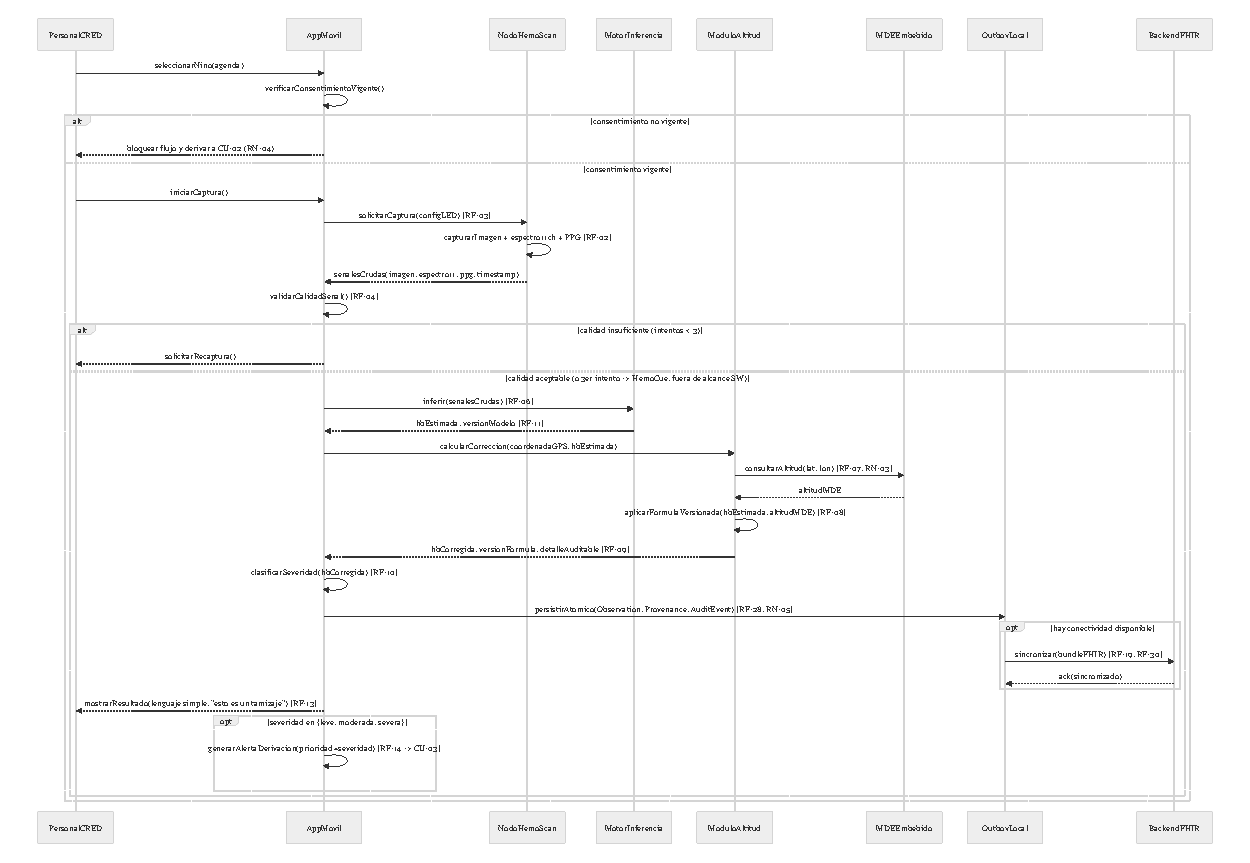
\includegraphics[width=1.0\linewidth,height=0.86\textheight,keepaspectratio]{assets/05-requerimientos/diagrama-07-secuencia-cu01.pdf}
\end{figure}

\textbf{Trazabilidad de este diagrama:} RF-01 a RF-14, RF-18, RF-19, RF-28; RN-01 a RN-05, RN-10; RNF-01, RNF-03, RNF-08. Corresponde íntegramente al flujo principal y al flujo alterno A1 de CU-01 (sección 1.6).

\textbf{Diagrama 8 --- Secuencia de CU-02: Registrar y revocar consentimiento informado digital.}

\begin{figure}[H]
\centering
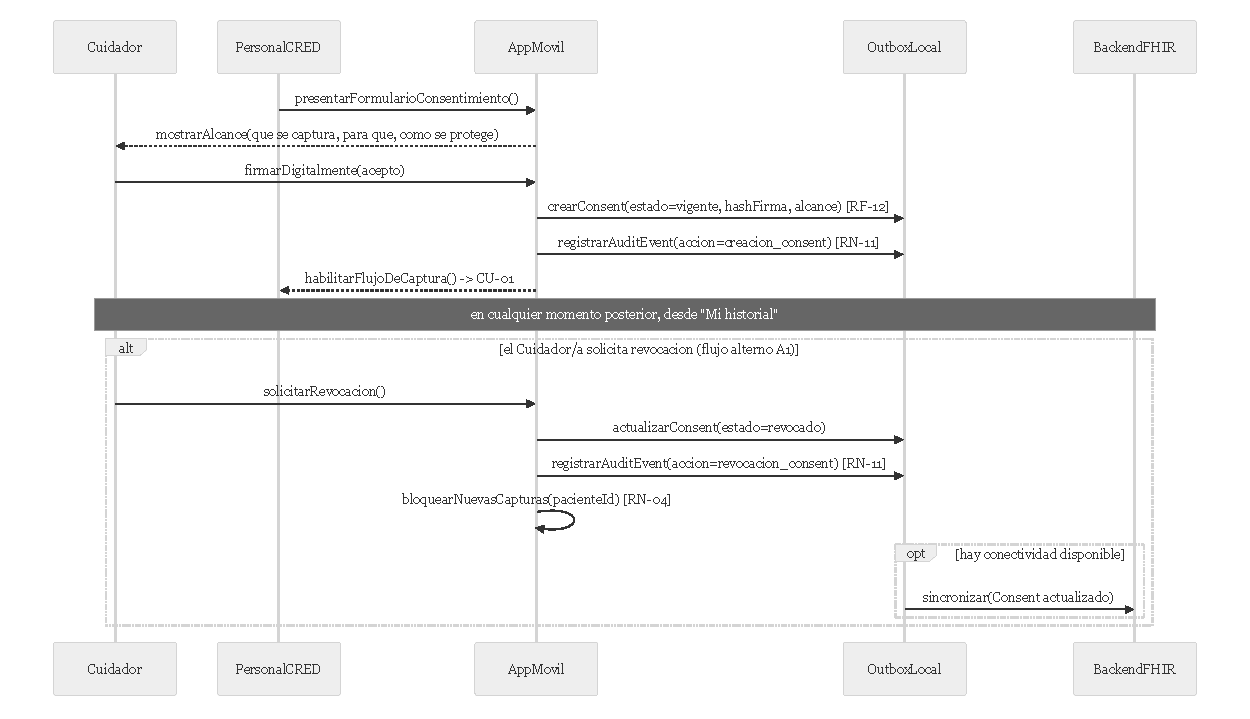
\includegraphics[width=0.8\linewidth,height=0.86\textheight,keepaspectratio]{assets/05-requerimientos/diagrama-08-secuencia-cu02.pdf}
\end{figure}

\textbf{Trazabilidad de este diagrama:} RF-12; RN-04, RN-11; RNF-07, RNF-19. El flujo alterno de revocación materializa directamente el hallazgo H2 de la validación heurística (sección 2.5 y Anexo C).

\textbf{Diagrama 9 --- Secuencia de CU-03: Confirmar o descartar diagnóstico de anemia (supervisión humana obligatoria).}

\begin{figure}[H]
\centering
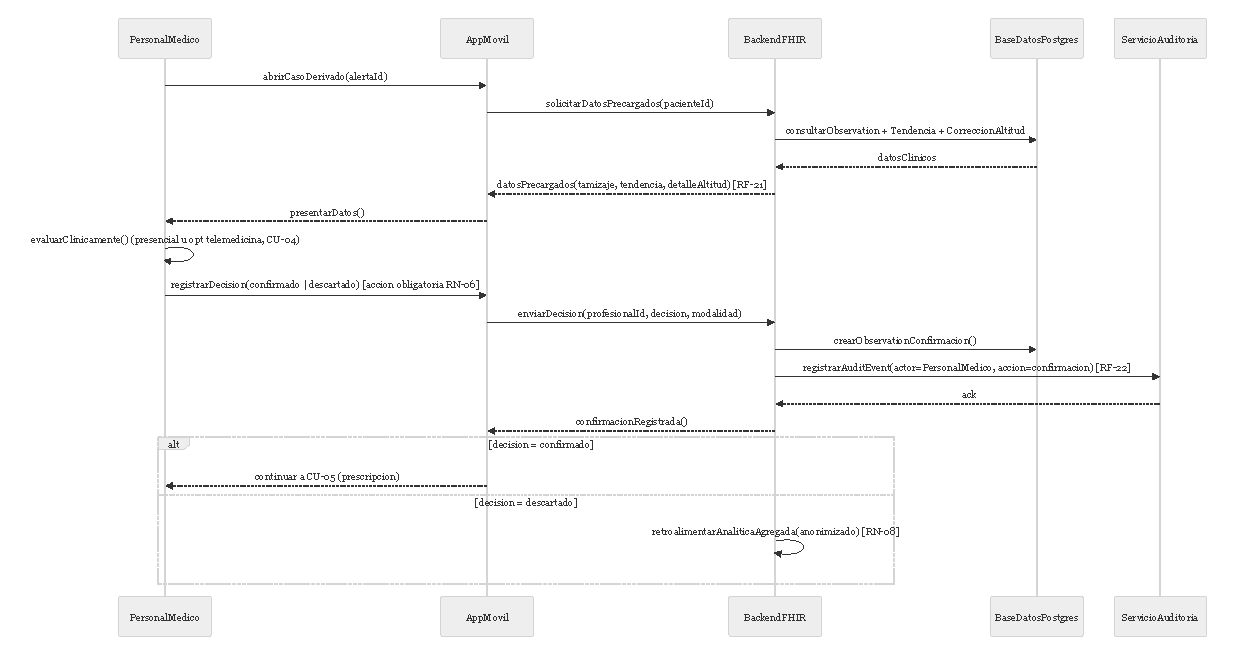
\includegraphics[width=0.92\linewidth,height=0.86\textheight,keepaspectratio]{assets/05-requerimientos/diagrama-09-secuencia-cu03.pdf}
\end{figure}

\textbf{Trazabilidad de este diagrama:} RF-21, RF-22; RN-01, RN-06, RN-10; RNF-08, RNF-09. \textbf{Nota de honestidad técnica:} en el 100 \% de las trayectorias posibles de este diagrama, el paso ``registrarDecision'' exige una acción humana explícita del Personal médico; no existe ninguna rama en la que el sistema confirme o descarte automáticamente, en cumplimiento literal del principio ``tamizaje, nunca diagnóstico autónomo'' (RN-01) y del DS 115-2025-PCM.

\textbf{Diagrama 10 --- Secuencia de CU-08: Sincronización diferida de recursos FHIR (proceso automático offline-first).}

\begin{figure}[H]
\centering
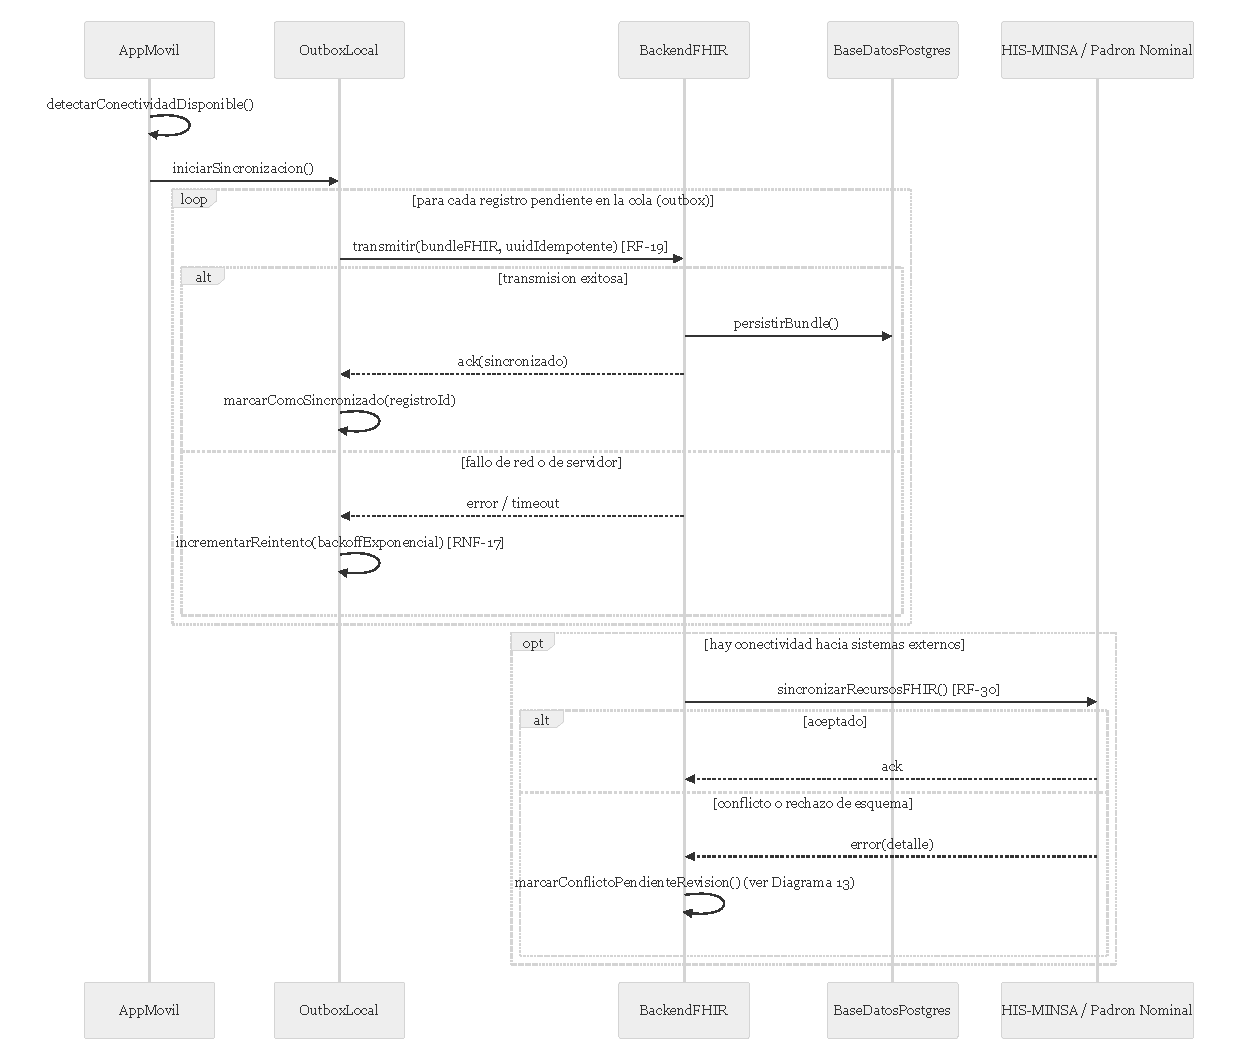
\includegraphics[width=0.92\linewidth,height=0.86\textheight,keepaspectratio]{assets/05-requerimientos/diagrama-10-secuencia-cu08.pdf}
\end{figure}

\textbf{Trazabilidad de este diagrama:} RF-19, RF-28, RF-29, RF-30; RN-05, RN-09; RNF-03, RNF-04, RNF-17. Este diagrama es la materialización operativa directa de ADR-01 (arquitectura offline-first con patrón \emph{outbox}).

\subsection{4.4 Diagramas de estados}\label{diagramas-de-estados}

Se desarrollan tres diagramas de estados, seleccionados por representar cada uno un eje distinto de la criticidad del sistema: el ciclo de vida clínico completo de una determinación (el artefacto de mayor valor y mayor riesgo regulatorio del sistema), el ciclo de vida del consentimiento (el control de cumplimiento normativo que activa/desactiva todo el flujo) y el ciclo de vida de un registro de sincronización (la materialización de la arquitectura offline-first). Los tres se derivan directamente de los estados y transiciones ya implícitos en los flujos principales y alternos de los casos de uso de la sección 1.6 y en las reglas de negocio de la sección 1.4.

\textbf{Notación (aplica a los tres diagramas de esta sección).} \emph{(Renderizados a imagen vectorial desde una especificación \texttt{stateDiagram} de diagrama-como-código, con un renderizador libre de licencia.)} \texttt{{[}*{]}} estado inicial o final; \texttt{-\/-\textgreater{}} transición; \texttt{{[}guarda{]}} condición que habilita la transición (incluida como parte del texto de la transición); \texttt{/\ acción} efecto que dispara la transición.

\textbf{Diagrama 11 --- Estados del ciclo de vida de una Determinación (recurso Observation).}

\begin{figure}[H]
\centering
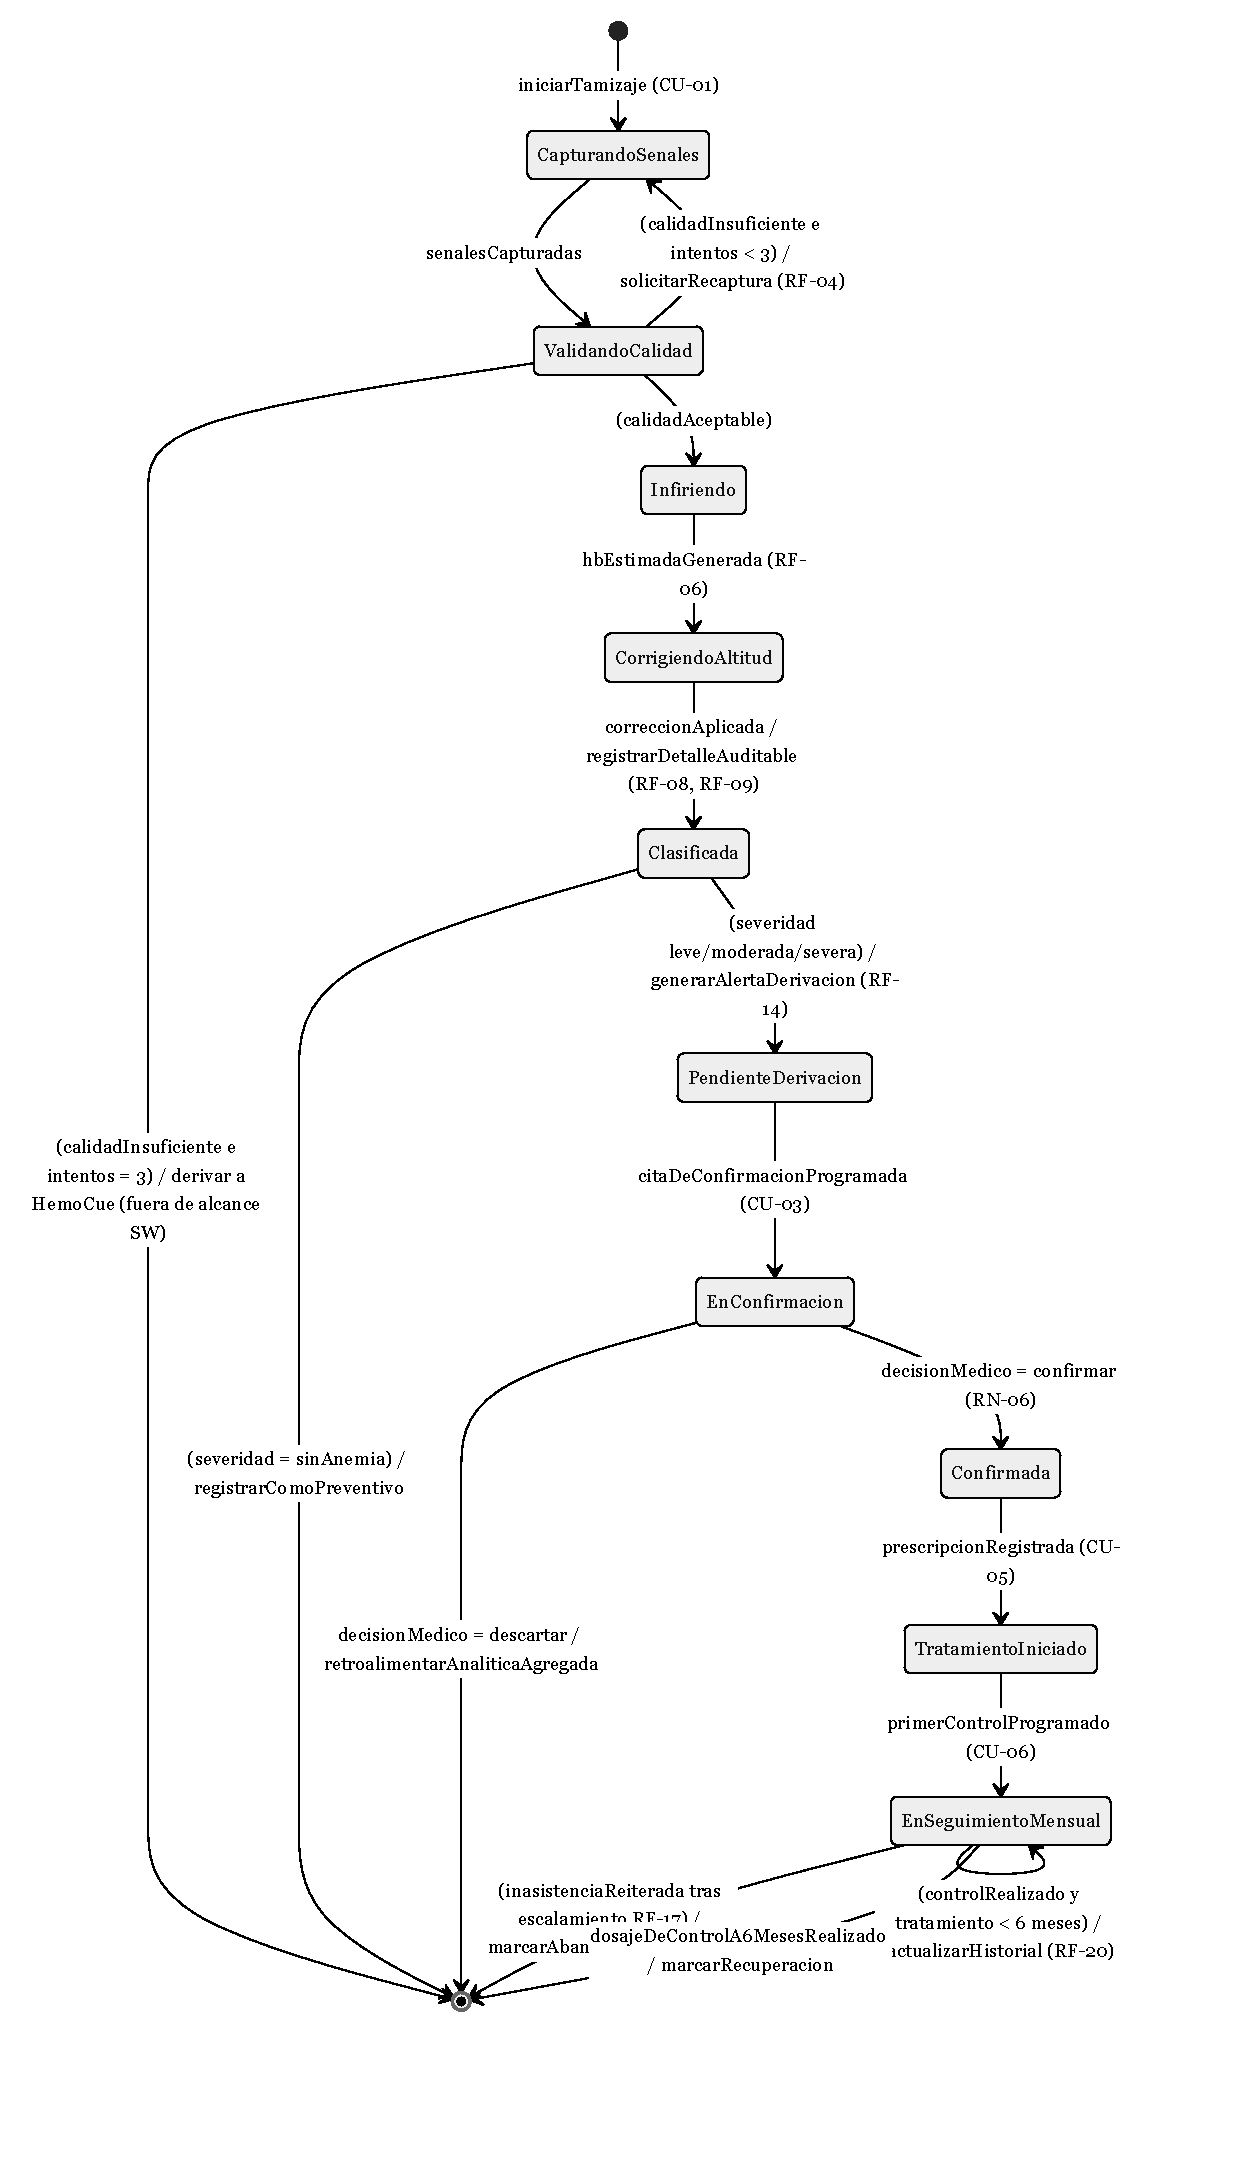
\includegraphics[width=0.85\linewidth,height=0.86\textheight,keepaspectratio]{assets/05-requerimientos/diagrama-11-estados-determinacion.pdf}
\end{figure}

\textbf{Nota de diseño (estado transversal no representado como región concurrente).} Por simplicidad de la notación adoptada para este diagrama, no se representa formalmente una región de estado concurrente (\emph{orthogonal region}), propia de la notación gráfica estándar de UML. En la práctica, desde el estado \texttt{CapturandoSeñales} en adelante, cada Determinación mantiene en paralelo un sub-estado de sincronización independiente (\texttt{PendienteSincronizacion} / \texttt{Sincronizado}, ver Diagrama 13), gobernado por la disponibilidad de conectividad y no por la lógica clínica de este diagrama; ambos ejes de estado son ortogonales entre sí por diseño (ADR-01).

\textbf{Trazabilidad de este diagrama:} RF-04, RF-06 a RF-10, RF-14, RF-17, RF-20 a RF-22, RF-24; RN-01, RN-06, RN-10; cubre la totalidad del recorrido de CU-01, CU-03, CU-05 y CU-06.

\textbf{Diagrama 12 --- Estados del ciclo de vida del Consentimiento (recurso Consent).}

\begin{figure}[H]
\centering
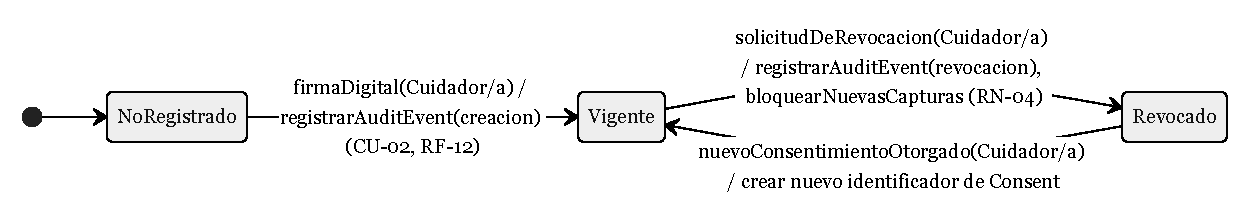
\includegraphics[width=0.95\linewidth,height=0.86\textheight,keepaspectratio]{assets/05-requerimientos/diagrama-12-estados-consentimiento.pdf}
\end{figure}

\textbf{Nota de diseño.} Este es, deliberadamente, el diagrama de estados más simple de los tres: su simplicidad refleja una decisión de diseño explícita (RN-04) de que solo dos estados estables (\texttt{Vigente}, \texttt{Revocado}) son suficientes para bloquear o habilitar de forma binaria el resto del sistema, evitando estados intermedios ambiguos que pudieran introducir zonas grises de cumplimiento de la Ley N.° 29733.

\textbf{Trazabilidad de este diagrama:} RF-12; RN-04, RN-11; RNF-07, RNF-19. Corresponde íntegramente a CU-02.

\textbf{Diagrama 13 --- Estados de un registro de sincronización FHIR (cola de Outbox).}

\begin{figure}[H]
\centering
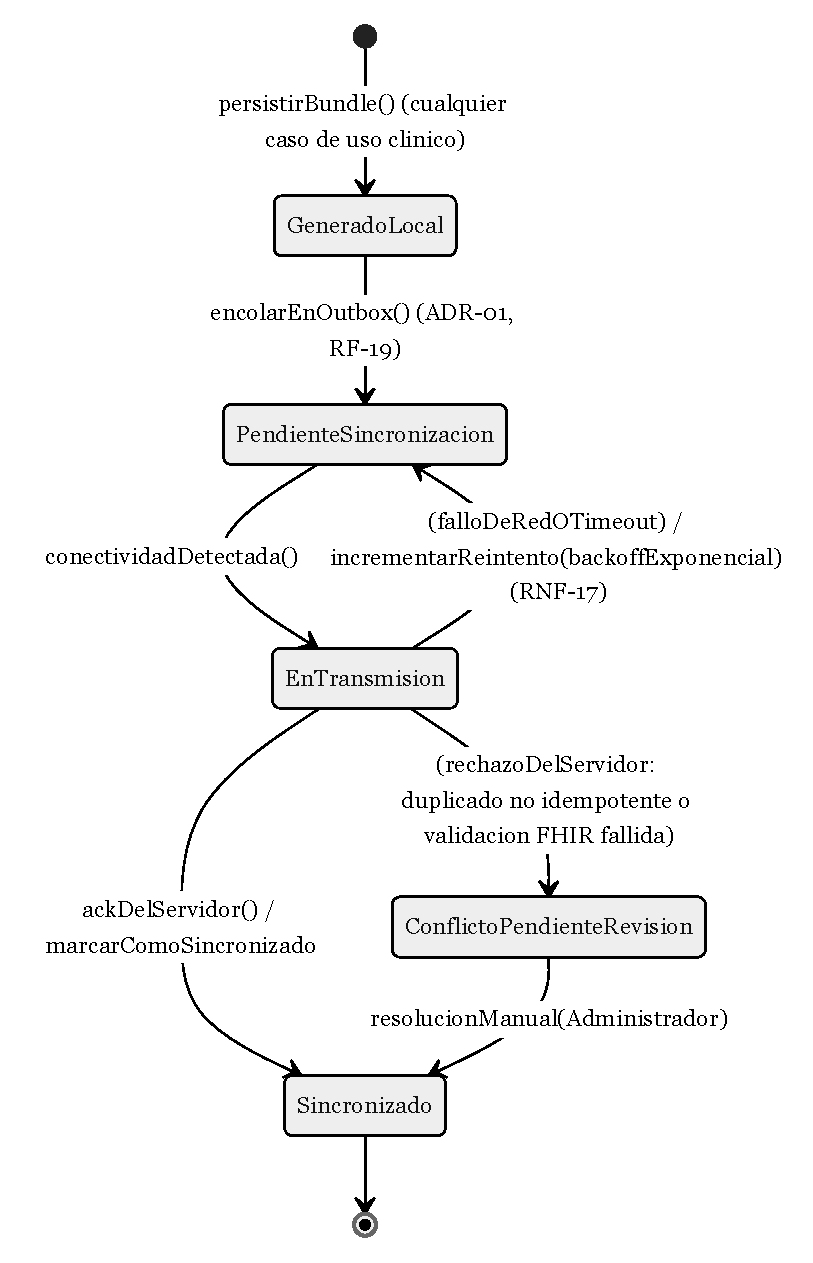
\includegraphics[width=0.9\linewidth,height=0.86\textheight,keepaspectratio]{assets/05-requerimientos/diagrama-13-estados-sincronizacion.pdf}
\end{figure}

\textbf{Trazabilidad de este diagrama:} RF-19, RF-28 a RF-30; RN-05; RNF-03, RNF-04, RNF-17. Es la contraparte de estados del Diagrama 10 (secuencia de CU-08): mientras el Diagrama 10 muestra el orden temporal de los mensajes de sincronización, este diagrama muestra los estados estables por los que transita cada registro individual de la cola.

\subsection{4.5 Modelo de datos detallado y mapeo a los seis recursos FHIR}\label{modelo-de-datos-detallado-y-mapeo-a-los-seis-recursos-fhir}

Esta subsección consolida el diagrama de clases de la sección 4.2 en un modelo de diseño detallado orientado específicamente a su serialización como recursos HL7 FHIR, requisito mandatorio del proyecto (RF-28 a RF-31, RNF-10) y condición habilitante de toda interoperabilidad con el HIS-MINSA y el Padrón Nominal. La tabla siguiente mapea cada uno de los seis recursos FHIR ya adoptados por el proyecto (Observation, Provenance, AuditEvent, Consent, Device, Patient) contra las clases internas de origen del Diagrama 6.

{\small
\begin{longtable}[]{@{}
  >{\raggedright\arraybackslash}p{(\linewidth - 8\tabcolsep) * \real{0.2000}}
  >{\raggedright\arraybackslash}p{(\linewidth - 8\tabcolsep) * \real{0.2000}}
  >{\raggedright\arraybackslash}p{(\linewidth - 8\tabcolsep) * \real{0.2000}}
  >{\raggedright\arraybackslash}p{(\linewidth - 8\tabcolsep) * \real{0.2000}}
  >{\raggedright\arraybackslash}p{(\linewidth - 8\tabcolsep) * \real{0.2000}}@{}}
\toprule\noalign{}
\begin{minipage}[b]{\linewidth}\raggedright
Recurso FHIR
\end{minipage} & \begin{minipage}[b]{\linewidth}\raggedright
Clase(s) interna(s) de origen (Diagrama 6)
\end{minipage} & \begin{minipage}[b]{\linewidth}\raggedright
Elementos FHIR principales utilizados
\end{minipage} & \begin{minipage}[b]{\linewidth}\raggedright
Extensión/perfil requerido
\end{minipage} & \begin{minipage}[b]{\linewidth}\raggedright
Recursos FHIR relacionados
\end{minipage} \\
\midrule\noalign{}
\endhead
\bottomrule\noalign{}
\endlastfoot
\textbf{Patient} & Paciente & \texttt{identifier} (código Padrón Nominal), \texttt{birthDate}, \texttt{gender}, \texttt{managingOrganization} (establecimiento asignado) & Perfil FHIR peruano oficial, si existe --- \textbf{{[}DATO PENDIENTE DE VALIDAR: perfil FHIR-PE o guía de implementación oficial del MINSA, si existe{]}} & Referenciado por \texttt{Consent.patient} y \texttt{Observation.subject} \\
\textbf{Consent} & Consentimiento & \texttt{status} (vigente-\textgreater{}\emph{active}, revocado-\textgreater{}\emph{inactive}), \texttt{patient}, \texttt{dateTime}, \texttt{provision.actor} (Cuidador/a), \texttt{sourceAttachment} (evidencia de firma digital) & Extensión propuesta: rol/parentesco del firmante (madre, padre o tutor) & Precondición obligatoria de \texttt{Observation} (RN-04) \\
\textbf{Device} & Dispositivo (nodo) & \texttt{identifier} (número de serie), \texttt{version} (versión de firmware), \texttt{status} & Extensión propuesta: fecha de última calibración & Referenciado por \texttt{Observation.device} \\
\textbf{Observation} & Captura + CorreccionAltitud + Determinacion + CasoConfirmacion + Prescripcion (anotación, ADR-06) & \texttt{code} (hemoglobina; código LOINC exacto \textbf{{[}DATO PENDIENTE DE VALIDAR{]}}), \texttt{valueQuantity} (hbCorregida), \texttt{component} (hbObservada, altitudMDE, versionFormula), \texttt{interpretation} (severidad), \texttt{note} (prescripción estructurada), \texttt{status} & \textbf{Extensión propia y obligatoria del proyecto} \texttt{correccion-altitud} (altitud MDE, versión de fórmula, valor antes/después) --- no existe en el núcleo estándar de FHIR; materializa RN-02 y RF-09 & Referencia a \texttt{Patient} y \texttt{Device}; es objetivo (\texttt{target}) de \texttt{Provenance} y de \texttt{AuditEvent} \\
\textbf{Provenance} & CorreccionAltitud (agente = sistema/algoritmo), CasoConfirmacion (agente = Personal médico) & \texttt{target} (Observation referenciada), \texttt{agent} (tipo: dispositivo, algoritmo o persona, con rol), \texttt{activity}, \texttt{recorded} & --- (uso estándar del recurso) & Siempre apunta a un \texttt{Observation} \\
\textbf{AuditEvent} & AuditEvent & \texttt{agent} (actor autenticado), \texttt{action} (C/R/U/D), \texttt{entity} (recurso afectado, cualquiera de los cinco anteriores), \texttt{recorded}, \texttt{outcome} & --- (uso estándar del recurso) & Puede referenciar a cualquiera de los otros cinco recursos, sin excepción (RN-11) \\
\end{longtable}
}

\textbf{Diagrama 14 --- Relaciones entre los seis recursos FHIR del proyecto (vista complementaria a la sección 4.2).}

\begin{figure}[H]
\centering
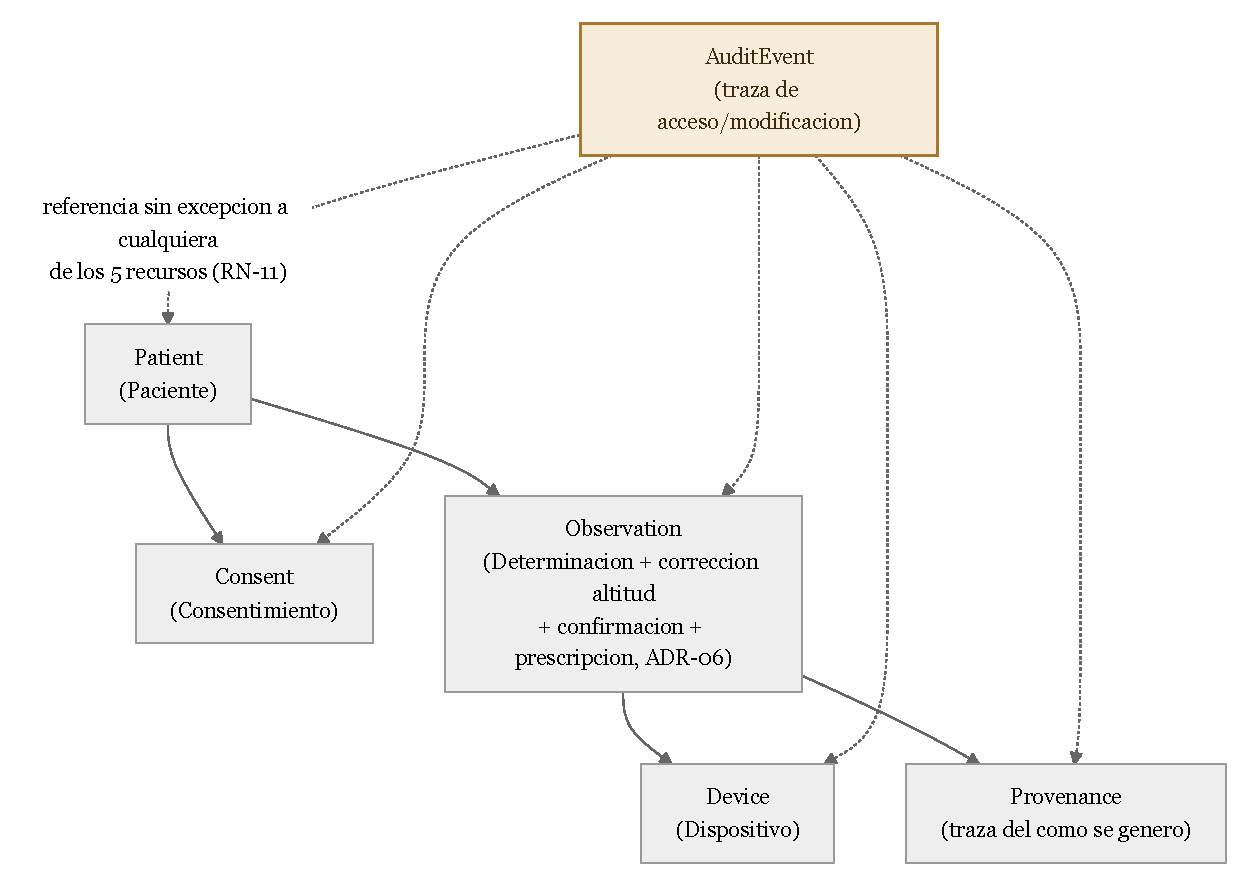
\includegraphics[width=0.7\linewidth,height=0.86\textheight,keepaspectratio]{assets/05-requerimientos/diagrama-14-recursos-fhir.pdf}
\end{figure}

El mapeo anterior evidencia que \textbf{Observation es, con claridad, el recurso de mayor complejidad de modelado del proyecto}: concentra la captura, la corrección por altitud, la clasificación de severidad, la confirmación clínica y ---en Fase 0--- la anotación de prescripción (ADR-06). El estándar HL7 FHIR permite representar esta concentración mediante el elemento \texttt{component} (para las submediciones de la corrección) y mediante una extensión propia (para el detalle auditable de altitud), en lugar de fragmentar cada paso en un recurso no estandarizado. Esta decisión de modelado no es arbitraria: es la consecuencia directa de ADR-05 (autocalibración por altitud como módulo independiente pero auditable) y de RN-02, y debe validarse formalmente contra un validador de esquema FHIR (por ejemplo, el validador oficial de HL7) antes de la construcción --- verificación que, consistente con el alcance de este entregable como ejercicio previo a la construcción, no se ha ejecutado todavía.

Dos parámetros de esta sección permanecen, de forma consistente con el resto del documento, marcados explícitamente como pendientes de validar: la versión exacta del estándar FHIR a adoptar (R4 frente a R5, ya señalado en RNF-10) y el código LOINC exacto del analito de hemoglobina no invasiva estimada, que podría requerir, de hecho, un código distinto al de la hemoglobina capilar medida por HemoCue, por tratarse de una estimación óptica indirecta y no de una medición directa de laboratorio --- matiz que el equipo no ha resuelto y que queda para la etapa de implementación, en coordinación con el HIS-MINSA real una vez exista convenio institucional.

La matriz de trazabilidad completa de los 40 requerimientos funcionales y las 12 reglas de negocio se presenta en el \textbf{Anexo D}; el índice completo de los quince diagramas de este documento, junto con un diagrama complementario de paquetes del backend, se presenta en el \textbf{Anexo E}.

\begin{center}\rule{0.5\linewidth}{0.5pt}\end{center}

\section{Anexos}\label{anexos}

\subsection{Anexo A --- Glosario de términos técnicos de este entregable}\label{anexo-a-glosario-de-tuxe9rminos-tuxe9cnicos-de-este-entregable}

{\small
\begin{longtable}[]{@{}
  >{\raggedright\arraybackslash}p{(\linewidth - 2\tabcolsep) * \real{0.5000}}
  >{\raggedright\arraybackslash}p{(\linewidth - 2\tabcolsep) * \real{0.5000}}@{}}
\toprule\noalign{}
\begin{minipage}[b]{\linewidth}\raggedright
Término
\end{minipage} & \begin{minipage}[b]{\linewidth}\raggedright
Definición breve
\end{minipage} \\
\midrule\noalign{}
\endhead
\bottomrule\noalign{}
\endlastfoot
ADR (Architecture Decision Record) & Registro estructurado de una decisión arquitectónica, con su contexto, la decisión tomada, sus consecuencias y las alternativas consideradas (sección 3.5) \\
BLE / GATT & Bluetooth Low Energy y su protocolo de atributos genéricos (\emph{Generic Attribute Profile}), usado para la comunicación entre el nodo HemoScan Andino y la app móvil \\
Bundle FHIR & Contenedor estándar de HL7 FHIR que agrupa varios recursos (p.~ej., Observation + Provenance + AuditEvent) para transmitirlos de forma atómica \\
CA (Criterio de Aceptación) & Condición formal, expresada en formato Given/When/Then, que determina si un requerimiento se considera satisfecho (sección 1.8) \\
CU (Caso de Uso) & Descripción estructurada de una interacción completa entre un actor y el sistema para lograr un objetivo (sección 1.6) \\
Edge inference / inferencia en el borde & Ejecución del modelo de aprendizaje automático directamente en el dispositivo del usuario final, sin depender de un servidor remoto \\
FHIR (Fast Healthcare Interoperability Resources) & Estándar de HL7 para el intercambio electrónico de información de salud mediante recursos estructurados (Observation, Patient, Consent, etc.) \\
GWR / MGWR & Regresión Ponderada Geográficamente y su variante multiescala; técnicas de analítica espacial ya referenciadas en el Entregable N.° 2 y retomadas en RF-34 \\
H3 & Sistema de indexación geoespacial jerárquico basado en hexágonos (Uber), usado para agregar datos de forma anonimizada (RN-08) \\
HL7 & Health Level Seven International, organización que desarrolla el estándar FHIR \\
LOINC & \emph{Logical Observation Identifiers Names and Codes}; sistema de codificación estándar para observaciones clínicas y de laboratorio \\
MDE (Modelo Digital de Elevación) & Representación digital de la altitud del terreno, consultada por coordenada geográfica para la corrección de hemoglobina (RF-07, RN-03) \\
MoSCoW & Técnica de priorización de requerimientos (\emph{Must, Should, Could, Won't}), usada en la columna ``Prioridad'' de las secciones 1.2 y 1.3 \\
Offline-first & Estilo arquitectónico en el que la aplicación se diseña para funcionar de forma completa sin conectividad, sincronizando de forma diferida cuando esta existe (ADR-01) \\
OIDC (OpenID Connect) & Protocolo de autenticación basado en OAuth 2.0, usado por Keycloak para centralizar la identidad del sistema (ADR-09) \\
ONNX / ONNX Runtime & \emph{Open Neural Network Exchange}; formato abierto para modelos de aprendizaje automático y su motor de ejecución multiplataforma (ADR-04) \\
Outbox pattern & Patrón de diseño que encola localmente las escrituras pendientes de sincronización, garantizando que ninguna se pierda ante fallos de red (ADR-01) \\
PMTiles & Formato de archivo único y estático para servir mapas vectoriales sin necesidad de un servidor de teselas dedicado, usado junto con MapLibre GL JS \\
PWA (Progressive Web App) & Aplicación web que puede instalarse y operar con capacidades similares a una aplicación nativa, incluyendo funcionamiento offline \\
RBAC (Role-Based Access Control) & Modelo de control de acceso basado en roles, implementado mediante Keycloak (RNF-06, RF-37) \\
RF / RNF / RN & Siglas de este documento para Requerimiento Funcional, Requerimiento No Funcional y Regla de Negocio, respectivamente \\
SRS (Software Requirements Specification) & Documento formal de especificación de requerimientos de software; este Entregable N.° 5 cumple ese rol para HemoScan Andino \\
TFLite (TensorFlow Lite) & Formato y motor de inferencia de Google optimizado para dispositivos móviles y embebidos, adoptado como ruta alterna de despliegue (ADR-04) \\
UML (Unified Modeling Language) & Lenguaje unificado de modelado; sus notaciones (casos de uso, clases, secuencia, estados) se representan en este documento en forma textual (sección 4) \\
Walkthrough cognitivo & Técnica de evaluación de usabilidad en la que un participante recorre tareas específicas verbalizando su razonamiento, usada en la validación del prototipo (sección 2.5, Anexo C) \\
\end{longtable}
}

\subsection{Anexo B --- Fuentes y referencias}\label{anexo-b-fuentes-y-referencias}

\textbf{Fuentes normativas y científicas del proyecto} (ya citadas y validadas en los Entregables N.° 1 a N.° 4; reutilizadas aquí sin modificación):
- ENDES 2025 --- prevalencia de anemia infantil de 56.1 \% en menores de 3 años en Puno.
- Gonzales, G. F. et al.~(2025) --- riesgo de sobrediagnóstico por corrección de hemoglobina en altitud.
- Baquerizo-Sedano, L. et al.~(2025) --- íd., evidencia complementaria sobre corrección de hemoglobina por altitud.
- NTS 213-MINSA/DGIESP-2024 --- Norma Técnica de Salud para el manejo de la anemia.
- DS 115-2025-PCM --- reglamento de la Ley N.° 31814 de inteligencia artificial (salud como sector de alto riesgo).
- Ley N.° 29733 --- Ley de Protección de Datos Personales.

\textbf{Fuentes y estándares técnicos de referencia general de la industria} (no específicos de la organización ni verificados contra el contexto exacto de la Microred de Salud Altiplano-Puno; se citan como respaldo de las decisiones de diseño, no como datos de la organización):
- HL7 FHIR (especificación R4/R5) --- hl7.org/fhir.
- ISO/IEC 25010:2011 --- modelo de calidad de producto de software, base de la sección 1.3.
- Nielsen, J. --- diez heurísticas de usabilidad (Nielsen Norman Group), base de la validación de la sección 2.5 y el Anexo C.
- Documentación oficial de ONNX Runtime Mobile y de TensorFlow Lite, para el diseño del motor de inferencia embebido.
- Documentación oficial de MapLibre GL JS, PMTiles y H3 (Uber), para el diseño del mapa de cobertura/riesgo.
- Documentación oficial de PySAL/esda (Getis-Ord Gi*, LISA), ya referenciada en el Entregable N.° 2.
- Documentación oficial de Flower (Federated Learning Framework) y de Keycloak (OIDC/RBAC).
- MoSCoW, como práctica estándar de priorización ágil, ya utilizada en el backlog del Entregable N.° 3.
- Cifra de referencia general de ancho de banda para videollamada de baja resolución (100-300 kbps), citada en la sección 1.9(a) como estimación de la industria, no como medición del territorio de la microred ilustrativa.

\textbf{Documentos internos del propio proyecto HemoScan Andino} (insumo directo y obligatorio de este entregable, según se declara en la Nota metodológica inicial):
- Entregable N.° 1 --- Diagnóstico Organizacional.
- Entregable N.° 2 --- Business Case.
- Entregable N.° 3 --- Plan de Gestión del Proyecto (EDT, cronograma, riesgos, backlog ágil de 25 historias de usuario).
- Entregable N.° 4 --- Modelado de Procesos AS-IS/TO-BE (14 automatizaciones A1-A14, matriz de trazabilidad FHIR por etapa).

\subsection{Anexo C --- Acta de validación heurística interna y recorrido cognitivo exploratorio (no equivalente a una validación con stakeholders reales)}\label{anexo-c-acta-de-validaciuxf3n-heuruxedstica-interna-y-recorrido-cognitivo-exploratorio-no-equivalente-a-una-validaciuxf3n-con-stakeholders-reales}

\begin{quote}
\textbf{Nota de nomenclatura (aclarada en esta revisión).} Este anexo se renombra explícitamente en esta revisión, de ``Acta de validación del prototipo'' a la denominación anterior, para eliminar cualquier ambigüedad frente al lector de la rúbrica: la plantilla del producto exige una \textbf{acta de validación con stakeholders}, y lo aquí documentado es una \textbf{evaluación heurística interna del propio equipo} más un \textbf{recorrido cognitivo con voluntarios ajenos a la organización}, no una validación con stakeholders reales de la Microred de Salud Altiplano-Puno. Esta distinción ya se declaraba en el cuerpo del acta (ver ``Limitación declarada explícitamente'' más abajo); el cambio de título simplemente la hace inequívoca desde el índice del documento.
\end{quote}

\textbf{Datos generales.} Documento: acta de validación interna del prototipo navegable de HemoScan Andino. Fecha (supuesta, a confirmar con el cronograma real del sprint correspondiente): semana del hito H3 del Entregable N.° 3 (fin de diseño, Mes 4). Modalidad: remota, mediante recorrido guiado de los wireframes textuales sobre videollamada. Responsable de la sesión: Integrante 3 (Líder de Ingeniería de Software).

\textbf{Objetivo.} Identificar defectos gruesos de usabilidad, claridad de lenguaje y coherencia de navegación en el prototipo de baja/media fidelidad (sección 2) antes de comprometer esfuerzo de construcción, en ausencia de acceso a usuarios finales reales de la Microred de Salud Altiplano-Puno.

\textbf{Metodología.} Se aplicaron dos técnicas complementarias:
1. \textbf{Evaluación heurística interna:} los 3 integrantes del equipo aplicaron, de forma independiente, una adaptación de las 10 heurísticas de usabilidad de Nielsen a las 23 pantallas del prototipo (16 de app móvil, 7 de plataforma web), consolidando hallazgos en una sesión conjunta posterior.
2. \textbf{Recorrido cognitivo (\emph{cognitive walkthrough}):} 3 personas voluntarias, ajenas al equipo y a la carrera de Ingeniería de Sistemas, recorrieron paso a paso los flujos CU-01 (tamizaje), CU-02 (consentimiento) y CU-03 (confirmación) sobre los wireframes textuales presentados como láminas, verbalizando en voz alta su razonamiento en cada pantalla.

\textbf{Participantes.} Se declara explícitamente que ninguno de los participantes es personal de salud real, cuidador/a real ni autoridad real de una microred; sus perfiles se anonimizan y se describen solo de forma funcional, dado que actuaron como \emph{proxies} exploratorios y no como stakeholders representativos:

{\small
\begin{longtable}[]{@{}
  >{\raggedright\arraybackslash}p{(\linewidth - 4\tabcolsep) * \real{0.3333}}
  >{\raggedright\arraybackslash}p{(\linewidth - 4\tabcolsep) * \real{0.3333}}
  >{\raggedright\arraybackslash}p{(\linewidth - 4\tabcolsep) * \real{0.3333}}@{}}
\toprule\noalign{}
\begin{minipage}[b]{\linewidth}\raggedright
Participante
\end{minipage} & \begin{minipage}[b]{\linewidth}\raggedright
Perfil funcional (no identificable)
\end{minipage} & \begin{minipage}[b]{\linewidth}\raggedright
Rol simulado en el recorrido
\end{minipage} \\
\midrule\noalign{}
\endhead
\bottomrule\noalign{}
\endlastfoot
Integrante 1 & Estudiante de Ingeniería de Sistemas, área de Infraestructura Tecnológica & Evaluador heurístico (las 23 pantallas) \\
Integrante 2 & Estudiante de Ingeniería de Sistemas, área de Gestión de TI & Evaluador heurístico (las 23 pantallas) \\
Integrante 3 & Estudiante de Ingeniería de Sistemas, área de Ingeniería de Software & Evaluador heurístico (las 23 pantallas) y facilitador de la sesión \\
Participante voluntario 1 & Persona adulta ajena al equipo, sin formación en salud ni en sistemas & Proxy de ``Cuidador/a'' en CU-02 \\
Participante voluntario 2 & Persona adulta ajena al equipo, con experiencia previa en atención al público (no de salud) & Proxy de ``Personal CRED'' en CU-01 \\
Participante voluntario 3 & Persona adulta ajena al equipo, sin formación en salud ni en sistemas & Proxy de ``Personal médico'' en CU-03 (únicamente para evaluar claridad de la interfaz, no la validez clínica de la decisión) \\
\end{longtable}
}

\textbf{Agenda de la sesión (duración total aproximada: 2 horas).}
1. (20 min) Presentación del propósito del prototipo y advertencia explícita de que se trata de wireframes textuales, no de una app funcional.
2. (40 min) Recorrido cognitivo guiado de CU-01, CU-02 y CU-03 con los 3 participantes voluntarios, de forma individual y secuencial.
3. (30 min) Aplicación de las 10 heurísticas de Nielsen por los 3 integrantes del equipo sobre las 23 pantallas.
4. (30 min) Consolidación conjunta de hallazgos y priorización de correcciones.

\textbf{Hallazgos y correcciones aplicadas.} Los siete hallazgos siguientes ya se resumieron en la sección 2.5; se presenta aquí el detalle ampliado con la técnica y el/los participante(s) que lo detectaron:

{\small
\begin{longtable}[]{@{}
  >{\raggedright\arraybackslash}p{(\linewidth - 12\tabcolsep) * \real{0.1429}}
  >{\raggedright\arraybackslash}p{(\linewidth - 12\tabcolsep) * \real{0.1429}}
  >{\raggedright\arraybackslash}p{(\linewidth - 12\tabcolsep) * \real{0.1429}}
  >{\raggedright\arraybackslash}p{(\linewidth - 12\tabcolsep) * \real{0.1429}}
  >{\raggedright\arraybackslash}p{(\linewidth - 12\tabcolsep) * \real{0.1429}}
  >{\raggedright\arraybackslash}p{(\linewidth - 12\tabcolsep) * \real{0.1429}}
  >{\raggedright\arraybackslash}p{(\linewidth - 12\tabcolsep) * \real{0.1429}}@{}}
\toprule\noalign{}
\begin{minipage}[b]{\linewidth}\raggedright
N.°
\end{minipage} & \begin{minipage}[b]{\linewidth}\raggedright
Hallazgo
\end{minipage} & \begin{minipage}[b]{\linewidth}\raggedright
Técnica / participante que lo detectó
\end{minipage} & \begin{minipage}[b]{\linewidth}\raggedright
Pantalla afectada
\end{minipage} & \begin{minipage}[b]{\linewidth}\raggedright
Severidad (escala interna 1-4)
\end{minipage} & \begin{minipage}[b]{\linewidth}\raggedright
Corrección aplicada
\end{minipage} & \begin{minipage}[b]{\linewidth}\raggedright
Estado
\end{minipage} \\
\midrule\noalign{}
\endhead
\bottomrule\noalign{}
\endlastfoot
H1 & Uso directo del término médico ``anémico'' & Heurística ``lenguaje del usuario'' (Integrante 2) & P09 & 3 --- alta (riesgo de alarma innecesaria) & Reemplazo por ``hemoglobina un poco más baja de lo esperado para tu edad'' & Corregido \\
H2 & No era evidente que el consentimiento pudiera revocarse & Recorrido cognitivo, Participante voluntario 1 & P05 / historial & 3 --- alta (riesgo de cumplimiento, Ley N.° 29733) & Botón explícito ``Revocar consentimiento'' en el historial & Corregido \\
H3 & El detalle técnico de la corrección por altitud saturaba la pantalla por defecto & Heurística ``estética y diseño minimalista'' (Integrante 3) & P09 & 2 --- media & Sección colapsable ``Ver detalle técnico'' & Corregido \\
H4 & No se identificaba el fin de la captura & Recorrido cognitivo, Participante voluntario 2 & P08 & 2 --- media & Indicador de progreso con retroalimentación háptica/sonora & Corregido \\
H5 & Alertas clínicas mezcladas con alertas de stock, sin distinción de prioridad & Heurística ``reconocimiento antes que recuerdo'' (Integrante 1) & P12 & 3 --- alta (riesgo de confundir prioridad clínica) & Separación en secciones con codificación de color e iconografía distinta & Corregido \\
H6 & Sin guía de recuperación ante fallo de emparejamiento BLE & Heurística ``ayuda para reconocer y recuperarse de errores'' (Integrante 1) & P06 & 2 --- media & Mensaje de error con pasos de recuperación explícitos & Corregido \\
H7 & Ícono de ``sin conexión'' confundido con un error & Recorrido cognitivo, Participante voluntario 2 & P16 & 1 --- baja & Etiqueta textual explícita junto al ícono & Corregido \\
\end{longtable}
}

\textbf{Conclusiones de la sesión.} Los 7 hallazgos identificados fueron corregidos en la versión del prototipo presentada en la sección 2 de este documento; no quedan hallazgos pendientes de la sesión sin resolver. La sesión no identificó defectos de severidad 4 (crítica/bloqueante).

\textbf{Limitación declarada explícitamente (léase junto con la sección 2.5).} Esta acta documenta una \textbf{validación interna de diseño}, útil para depurar errores gruesos de usabilidad, lenguaje y navegación antes de construir el sistema. \textbf{No constituye, bajo ninguna interpretación, una validación con stakeholders reales} de la Microred de Salud Altiplano-Puno (personal CRED, personal médico, cuidadores/as, Jefatura de microred o DIRESA/GERESA reales), dado que a la fecha de este entregable no existe convenio institucional que permita dicho acceso. Una futura acta de validación con stakeholders reales deberá, como mínimo, involucrar a un profesional CRED y a un profesional médico en ejercicio de un establecimiento de la microred real, y a un comité de ética constituido que revise el módulo de consentimiento --- \textbf{{[}DATO PENDIENTE DE VALIDAR: fecha y alcance de dicha validación real, sujeta a la firma del convenio institucional{]}}.

\textbf{Recomendación explícita antes de avanzar a construcción (añadida en esta revisión).} Dado que la firma de un convenio institucional formal con una microred real puede no concretarse antes del inicio de la construcción (Mes 5, hito H4 del Entregable N.° 3), el equipo recomienda gestionar, como mínimo, \textbf{una sesión de validación heurística/cognitiva adicional con un profesional CRED o un profesional médico real} ---aunque ejerza fuera de la Microred de Salud Altiplano-Puno ilustrativa, por ejemplo mediante una red de contactos personales o profesionales del equipo--- antes de comprometer el esfuerzo de construcción del Sprint 5 en adelante. Esta sesión no elevaría por sí sola el criterio de ``Validación con stakeholders'' a un nivel de rigor equivalente a una validación institucional plena, pero sí aportaría al menos una fuente de retroalimentación de un profesional de salud real sobre el lenguaje clínico, la severidad percibida y la usabilidad del flujo de confirmación (CU-03), cerrando parcialmente la brecha más severa identificada en este entregable con el menor costo de gestión posible.

\textbf{Firmas.} \textit{(Integrante 1 -- nombre por completar)} \_\_\_\_\_\_\_\_\_\_\_\_\_\_\_ · \textit{(Integrante 2 -- nombre por completar)} \_\_\_\_\_\_\_\_\_\_\_\_\_\_\_ · \textit{(Integrante 3 -- nombre por completar)} \_\_\_\_\_\_\_\_\_\_\_\_\_\_\_. \emph{(Se deja constancia de que no se recaban firmas de participantes voluntarios externos ni de personal institucional, por no ser stakeholders formales de la organización; solo se registra la conformidad interna del equipo con los hallazgos y correcciones de esta acta.)}

\subsection{Anexo D --- Matriz de trazabilidad de requerimientos}\label{anexo-d-matriz-de-trazabilidad-de-requerimientos}

Esta matriz traza los 40 requerimientos funcionales hacia los casos de uso (sección 1.6), las épicas/historias de usuario del Entregable N.° 3 (sección 1.7), las automatizaciones del Entregable N.° 4 (ya referenciadas en la sección 1.2) y la(s) pantalla(s) o componente(s) arquitectónico(s) que los materializan (secciones 2 y 3). Se organiza por los mismos ocho módulos (M1-M8) de la sección 1.2, para facilitar su verificación cruzada. La trazabilidad de los 20 requerimientos no funcionales hacia sus tácticas arquitectónicas ya se presentó de forma completa en la \textbf{sección 3.4} y no se duplica aquí.

\textbf{M1 --- Captura y firmware del nodo}

{\small
\begin{longtable}[]{@{}
  >{\raggedright\arraybackslash}p{(\linewidth - 8\tabcolsep) * \real{0.2000}}
  >{\raggedright\arraybackslash}p{(\linewidth - 8\tabcolsep) * \real{0.2000}}
  >{\raggedright\arraybackslash}p{(\linewidth - 8\tabcolsep) * \real{0.2000}}
  >{\raggedright\arraybackslash}p{(\linewidth - 8\tabcolsep) * \real{0.2000}}
  >{\raggedright\arraybackslash}p{(\linewidth - 8\tabcolsep) * \real{0.2000}}@{}}
\toprule\noalign{}
\begin{minipage}[b]{\linewidth}\raggedright
RF
\end{minipage} & \begin{minipage}[b]{\linewidth}\raggedright
CU relacionado
\end{minipage} & \begin{minipage}[b]{\linewidth}\raggedright
Épica / HU (Entregable N.° 3)
\end{minipage} & \begin{minipage}[b]{\linewidth}\raggedright
Automatización (Entregable N.° 4)
\end{minipage} & \begin{minipage}[b]{\linewidth}\raggedright
Pantalla / componente
\end{minipage} \\
\midrule\noalign{}
\endhead
\bottomrule\noalign{}
\endlastfoot
RF-01 & CU-01 (precondición) & E1 (HD01, HD02, HC01) & A1 & P06; {[}C: Firmware del Nodo{]} \\
RF-02 & CU-01 (paso 4) & E1 (HD01, HC01, HC02) & A1 & P07; {[}C: Firmware del Nodo{]} \\
RF-03 & CU-01 (paso 3-4) & E1 (HD02, HC02) & A1 & P07; {[}C: Firmware del Nodo{]} \\
RF-04 & CU-01 (paso 5, flujo A1) & E1 (HC03) & A1 (extensión propuesta) & P07; {[}C: App Móvil{]} \\
RF-05 & CU-01 (postcondición) & E1 (HC03) & Habilitante de A2/A5 & P16; {[}C: Base de datos local embebida{]} \\
\end{longtable}
}

\textbf{M2 --- Inferencia embebida y autocalibración por altitud}

{\small
\begin{longtable}[]{@{}
  >{\raggedright\arraybackslash}p{(\linewidth - 8\tabcolsep) * \real{0.2000}}
  >{\raggedright\arraybackslash}p{(\linewidth - 8\tabcolsep) * \real{0.2000}}
  >{\raggedright\arraybackslash}p{(\linewidth - 8\tabcolsep) * \real{0.2000}}
  >{\raggedright\arraybackslash}p{(\linewidth - 8\tabcolsep) * \real{0.2000}}
  >{\raggedright\arraybackslash}p{(\linewidth - 8\tabcolsep) * \real{0.2000}}@{}}
\toprule\noalign{}
\begin{minipage}[b]{\linewidth}\raggedright
RF
\end{minipage} & \begin{minipage}[b]{\linewidth}\raggedright
CU relacionado
\end{minipage} & \begin{minipage}[b]{\linewidth}\raggedright
Épica / HU (Entregable N.° 3)
\end{minipage} & \begin{minipage}[b]{\linewidth}\raggedright
Automatización (Entregable N.° 4)
\end{minipage} & \begin{minipage}[b]{\linewidth}\raggedright
Pantalla / componente
\end{minipage} \\
\midrule\noalign{}
\endhead
\bottomrule\noalign{}
\endlastfoot
RF-06 & CU-01 (paso 6) & E2 (HD04, HC04, HC05) & A2 & P08; {[}C: Motor de Inferencia{]} \\
RF-07 & CU-01 (paso 6) & E2 (HD06, HC06) & A3 & P09 (detalle técnico); {[}C: Módulo de Autocalibración por Altitud{]} \\
RF-08 & CU-01 (paso 7) & E2 (HD06, HC06) & A3 & P09; {[}C: Módulo de Autocalibración por Altitud{]} \\
RF-09 & CU-01 (paso 8); CU-10 & E2 (HC06) & A3, A14 & P09; W06; {[}C: Módulo de Autocalibración por Altitud{]} \\
RF-10 & CU-01 (paso 7-9) & E2 (HC04, HC05) & A6 (previo) & P09; {[}C: Motor de Inferencia{]} \\
RF-11 & CU-01 (transversal); CU-11 & E2 (HC17) & A14 & W07; {[}C: Registro de Versiones de Modelo{]} \\
\end{longtable}
}

\textbf{M3 --- Aplicación móvil: flujo de tamizaje y acompañamiento}

{\small
\begin{longtable}[]{@{}
  >{\raggedright\arraybackslash}p{(\linewidth - 8\tabcolsep) * \real{0.2000}}
  >{\raggedright\arraybackslash}p{(\linewidth - 8\tabcolsep) * \real{0.2000}}
  >{\raggedright\arraybackslash}p{(\linewidth - 8\tabcolsep) * \real{0.2000}}
  >{\raggedright\arraybackslash}p{(\linewidth - 8\tabcolsep) * \real{0.2000}}
  >{\raggedright\arraybackslash}p{(\linewidth - 8\tabcolsep) * \real{0.2000}}@{}}
\toprule\noalign{}
\begin{minipage}[b]{\linewidth}\raggedright
RF
\end{minipage} & \begin{minipage}[b]{\linewidth}\raggedright
CU relacionado
\end{minipage} & \begin{minipage}[b]{\linewidth}\raggedright
Épica / HU (Entregable N.° 3)
\end{minipage} & \begin{minipage}[b]{\linewidth}\raggedright
Automatización (Entregable N.° 4)
\end{minipage} & \begin{minipage}[b]{\linewidth}\raggedright
Pantalla / componente
\end{minipage} \\
\midrule\noalign{}
\endhead
\bottomrule\noalign{}
\endlastfoot
RF-12 & CU-02 & E3 (HC08) & A4 & P05; {[}C: App Móvil{]} \\
RF-13 & CU-01 (paso 9) & E3 (HC09) & Transversal (Entregable N.° 1) & P09; {[}C: App Móvil{]} \\
RF-14 & CU-01 (paso 10); CU-03 & E3 (HC09) & A6 & P12; {[}C: App Móvil{]} \\
RF-15 & Extensión de CU-01 (post-resultado) & E6 (HC14) & A8 & P10; {[}C: Motor de Reglas de Consejería{]} \\
RF-16 & CU-06 (paso 1) & E3 (HC12) & A10 & P11; {[}C: Servicio de Notificaciones{]} \\
RF-17 & CU-06 (flujo alterno A1) & E3 (HC12) & A11 & P12; {[}C: App Móvil{]} \\
RF-18 & Transversal (CU-01, CU-02, CU-06) & E3 (HC09) & Habilitante de A1-A3 & P16; {[}C: App Móvil{]} \\
RF-19 & CU-08 & E3/E4 (HC09, HC10) & A5 & P16; {[}C: Cola de Sincronización{]} \\
RF-20 & CU-06 (paso 3) & E3 (HC12) & A12 & P15; {[}C: App Móvil{]} \\
\end{longtable}
}

\textbf{M4 --- Confirmación clínica y extensión de telemedicina}

{\small
\begin{longtable}[]{@{}
  >{\raggedright\arraybackslash}p{(\linewidth - 8\tabcolsep) * \real{0.2000}}
  >{\raggedright\arraybackslash}p{(\linewidth - 8\tabcolsep) * \real{0.2000}}
  >{\raggedright\arraybackslash}p{(\linewidth - 8\tabcolsep) * \real{0.2000}}
  >{\raggedright\arraybackslash}p{(\linewidth - 8\tabcolsep) * \real{0.2000}}
  >{\raggedright\arraybackslash}p{(\linewidth - 8\tabcolsep) * \real{0.2000}}@{}}
\toprule\noalign{}
\begin{minipage}[b]{\linewidth}\raggedright
RF
\end{minipage} & \begin{minipage}[b]{\linewidth}\raggedright
CU relacionado
\end{minipage} & \begin{minipage}[b]{\linewidth}\raggedright
Épica / HU (Entregable N.° 3)
\end{minipage} & \begin{minipage}[b]{\linewidth}\raggedright
Automatización (Entregable N.° 4)
\end{minipage} & \begin{minipage}[b]{\linewidth}\raggedright
Pantalla / componente
\end{minipage} \\
\midrule\noalign{}
\endhead
\bottomrule\noalign{}
\endlastfoot
RF-21 & CU-03 (paso 1) & Derivada de E4 (HC10) & A6 & P13; {[}C: API Backend FHIR{]} \\
RF-22 & CU-03 (paso 3-4) & Derivada de E4/E5 & A14 & P13; {[}C: Servicio de Auditoría{]} \\
RF-23 & CU-04 (propuesta, no validada) & \textbf{Sin historia de usuario comprometida} (sección 1.7) & A7 & P14 (mockup); ADR-07 \\
RF-24 & CU-05 (paso 1) & Derivada de E4 & Extensión de ``Inicio de hierro'' (ADR-06) & P13 (extensión posterior a la confirmación --- ver nota) \\
\end{longtable}
}

\textbf{Nota sobre RF-24.} El flujo de prescripción se apoya en una extensión de la pantalla P13 (Confirmación clínica) para registrar la anotación estructurada; no se desarrolló como pantalla independiente entre las 23 wireframeadas en la sección 2. Se declara aquí, con la misma honestidad técnica del resto del documento, como una brecha menor de cobertura del prototipo, consistente con que la prescripción en Fase 0 es una anotación de Observation (ADR-06) y no un flujo de interfaz protagónico.

\textbf{M5 --- Farmacia y stock}

{\small
\begin{longtable}[]{@{}
  >{\raggedright\arraybackslash}p{(\linewidth - 8\tabcolsep) * \real{0.2000}}
  >{\raggedright\arraybackslash}p{(\linewidth - 8\tabcolsep) * \real{0.2000}}
  >{\raggedright\arraybackslash}p{(\linewidth - 8\tabcolsep) * \real{0.2000}}
  >{\raggedright\arraybackslash}p{(\linewidth - 8\tabcolsep) * \real{0.2000}}
  >{\raggedright\arraybackslash}p{(\linewidth - 8\tabcolsep) * \real{0.2000}}@{}}
\toprule\noalign{}
\begin{minipage}[b]{\linewidth}\raggedright
RF
\end{minipage} & \begin{minipage}[b]{\linewidth}\raggedright
CU relacionado
\end{minipage} & \begin{minipage}[b]{\linewidth}\raggedright
Épica / HU (Entregable N.° 3)
\end{minipage} & \begin{minipage}[b]{\linewidth}\raggedright
Automatización (Entregable N.° 4)
\end{minipage} & \begin{minipage}[b]{\linewidth}\raggedright
Pantalla / componente
\end{minipage} \\
\midrule\noalign{}
\endhead
\bottomrule\noalign{}
\endlastfoot
RF-25 & CU-05 (paso 2) & Derivada de E4 & A9 & Sin pantalla dedicada en Fase 0 (integración SIGA, Diagrama 5) \\
RF-26 & CU-05 (paso 4) & Derivada de E4 & A9 & P12; W02 \\
RF-27 & CU-05 (paso 4); CU-07 & Derivada de E7 & A9, A13 & W03 \\
\end{longtable}
}

\textbf{M6 --- Backend de interoperabilidad FHIR}

{\small
\begin{longtable}[]{@{}
  >{\raggedright\arraybackslash}p{(\linewidth - 8\tabcolsep) * \real{0.2000}}
  >{\raggedright\arraybackslash}p{(\linewidth - 8\tabcolsep) * \real{0.2000}}
  >{\raggedright\arraybackslash}p{(\linewidth - 8\tabcolsep) * \real{0.2000}}
  >{\raggedright\arraybackslash}p{(\linewidth - 8\tabcolsep) * \real{0.2000}}
  >{\raggedright\arraybackslash}p{(\linewidth - 8\tabcolsep) * \real{0.2000}}@{}}
\toprule\noalign{}
\begin{minipage}[b]{\linewidth}\raggedright
RF
\end{minipage} & \begin{minipage}[b]{\linewidth}\raggedright
CU relacionado
\end{minipage} & \begin{minipage}[b]{\linewidth}\raggedright
Épica / HU (Entregable N.° 3)
\end{minipage} & \begin{minipage}[b]{\linewidth}\raggedright
Automatización (Entregable N.° 4)
\end{minipage} & \begin{minipage}[b]{\linewidth}\raggedright
Pantalla / componente
\end{minipage} \\
\midrule\noalign{}
\endhead
\bottomrule\noalign{}
\endlastfoot
RF-28 & CU-01 (paso 8); transversal & E4 (HD03, HC10) & A5 & {[}C: API Backend FHIR{]} (sin pantalla propia) \\
RF-29 & CU-08 & E4 (HC10) & A5 & {[}C: API Backend FHIR{]} \\
RF-30 & CU-08 & E4 (HC10) & A5 & P16; {[}C: Conector HIS-MINSA/Padrón Nominal{]} \\
RF-31 & CU-10 & E4 (HC13) & A14 & W06; {[}C: Servicio de Auditoría{]} \\
RF-32 & CU-11 (inactivo Fase 0) & \textbf{Sin historia de usuario comprometida} (sección 1.7) & Capacidad nueva (ADR-08) & {[}C: Coordinador de Aprendizaje Federado{]} \\
\end{longtable}
}

\textbf{M7 --- Plataforma web}

{\small
\begin{longtable}[]{@{}
  >{\raggedright\arraybackslash}p{(\linewidth - 8\tabcolsep) * \real{0.2000}}
  >{\raggedright\arraybackslash}p{(\linewidth - 8\tabcolsep) * \real{0.2000}}
  >{\raggedright\arraybackslash}p{(\linewidth - 8\tabcolsep) * \real{0.2000}}
  >{\raggedright\arraybackslash}p{(\linewidth - 8\tabcolsep) * \real{0.2000}}
  >{\raggedright\arraybackslash}p{(\linewidth - 8\tabcolsep) * \real{0.2000}}@{}}
\toprule\noalign{}
\begin{minipage}[b]{\linewidth}\raggedright
RF
\end{minipage} & \begin{minipage}[b]{\linewidth}\raggedright
CU relacionado
\end{minipage} & \begin{minipage}[b]{\linewidth}\raggedright
Épica / HU (Entregable N.° 3)
\end{minipage} & \begin{minipage}[b]{\linewidth}\raggedright
Automatización (Entregable N.° 4)
\end{minipage} & \begin{minipage}[b]{\linewidth}\raggedright
Pantalla / componente
\end{minipage} \\
\midrule\noalign{}
\endhead
\bottomrule\noalign{}
\endlastfoot
RF-33 & CU-07 & E7 (HC15) & A13 & W03 \\
RF-34 & CU-07 & E7 (HC15) & A13 & W03 \\
RF-35 & CU-07 & E7 (HC15) & A12, A13 & W04 \\
RF-36 & CU-07 & E7 (HC15) & A12, A13 & W04 \\
RF-37 & CU-09 & E5 (HD08, HC07) & A14 & W05 \\
RF-38 & CU-10 & E4 (HC13) & A14 & W06 \\
\end{longtable}
}

\textbf{M8 --- Seguridad, cumplimiento y transversales}

{\small
\begin{longtable}[]{@{}
  >{\raggedright\arraybackslash}p{(\linewidth - 8\tabcolsep) * \real{0.2000}}
  >{\raggedright\arraybackslash}p{(\linewidth - 8\tabcolsep) * \real{0.2000}}
  >{\raggedright\arraybackslash}p{(\linewidth - 8\tabcolsep) * \real{0.2000}}
  >{\raggedright\arraybackslash}p{(\linewidth - 8\tabcolsep) * \real{0.2000}}
  >{\raggedright\arraybackslash}p{(\linewidth - 8\tabcolsep) * \real{0.2000}}@{}}
\toprule\noalign{}
\begin{minipage}[b]{\linewidth}\raggedright
RF
\end{minipage} & \begin{minipage}[b]{\linewidth}\raggedright
CU relacionado
\end{minipage} & \begin{minipage}[b]{\linewidth}\raggedright
Épica / HU (Entregable N.° 3)
\end{minipage} & \begin{minipage}[b]{\linewidth}\raggedright
Automatización (Entregable N.° 4)
\end{minipage} & \begin{minipage}[b]{\linewidth}\raggedright
Pantalla / componente
\end{minipage} \\
\midrule\noalign{}
\endhead
\bottomrule\noalign{}
\endlastfoot
RF-39 & Transversal (todos los CU) & E5 (HC11) & A14 & Sin pantalla propia; {[}C: Repositorio PostgreSQL/PostGIS{]} (Integrante 1) \\
RF-40 & Transversal; CU-01, CU-10 & E5 (HC11) & A14; DS 115-2025-PCM & W06; P09 \\
\end{longtable}
}

\textbf{Trazabilidad de las reglas de negocio (RN) hacia requerimientos, casos de uso y componente/ADR que las refuerza:}

{\small
\begin{longtable}[]{@{}
  >{\raggedright\arraybackslash}p{(\linewidth - 6\tabcolsep) * \real{0.2500}}
  >{\raggedright\arraybackslash}p{(\linewidth - 6\tabcolsep) * \real{0.2500}}
  >{\raggedright\arraybackslash}p{(\linewidth - 6\tabcolsep) * \real{0.2500}}
  >{\raggedright\arraybackslash}p{(\linewidth - 6\tabcolsep) * \real{0.2500}}@{}}
\toprule\noalign{}
\begin{minipage}[b]{\linewidth}\raggedright
RN
\end{minipage} & \begin{minipage}[b]{\linewidth}\raggedright
RF que la implementan
\end{minipage} & \begin{minipage}[b]{\linewidth}\raggedright
CU relacionado(s)
\end{minipage} & \begin{minipage}[b]{\linewidth}\raggedright
Componente / ADR que la refuerza arquitectónicamente
\end{minipage} \\
\midrule\noalign{}
\endhead
\bottomrule\noalign{}
\endlastfoot
RN-01 & RF-14, RF-21 & CU-01, CU-03 & Todos los ADR; principio rector transversal del producto \\
RN-02 & RF-08, RF-09, RF-11 & CU-01 & ADR-05; {[}C: Configuración Clínica{]} \\
RN-03 & RF-07 & CU-01 & ADR-05; {[}C: Módulo de Autocalibración por Altitud{]} \\
RN-04 & RF-12 & CU-02 & Diagrama 12 (estados de Consent) \\
RN-05 & RF-28 & CU-01, CU-08 & ADR-01 (patrón outbox, atomicidad) \\
RN-06 & RF-21, RF-22 & CU-03 & ADR-09 (RBAC vía Keycloak) \\
RN-07 & RF-15 & Extensión de CU-01 & {[}C: Motor de Reglas de Consejería{]} \\
RN-08 & RF-33 & CU-07 & Clase HexagonoCobertura (sección 4.2, sin FK a Paciente) \\
RN-09 & RF-32 & CU-11 & ADR-08 \\
RN-10 & RF-14, RF-17, RF-26 & CU-01, CU-05, CU-06 & Principio de supervisión humana (RNF-09) \\
RN-11 & RF-31, RF-38 & CU-10 & {[}C: Servicio de Auditoría{]} \\
RN-12 & RF-18 & CU-01, CU-02, CU-06 & ADR-01 \\
\end{longtable}
}

\subsection{Anexo E --- Índice de diagramas y diagrama complementario de paquetes del backend}\label{anexo-e-uxedndice-de-diagramas-y-diagrama-complementario-de-paquetes-del-backend}

\textbf{Índice completo de los quince diagramas del documento:}

{\small
\begin{longtable}[]{@{}
  >{\raggedright\arraybackslash}p{(\linewidth - 8\tabcolsep) * \real{0.2000}}
  >{\raggedright\arraybackslash}p{(\linewidth - 8\tabcolsep) * \real{0.2000}}
  >{\raggedright\arraybackslash}p{(\linewidth - 8\tabcolsep) * \real{0.2000}}
  >{\raggedright\arraybackslash}p{(\linewidth - 8\tabcolsep) * \real{0.2000}}
  >{\raggedright\arraybackslash}p{(\linewidth - 8\tabcolsep) * \real{0.2000}}@{}}
\toprule\noalign{}
\begin{minipage}[b]{\linewidth}\raggedright
N.°
\end{minipage} & \begin{minipage}[b]{\linewidth}\raggedright
Nombre
\end{minipage} & \begin{minipage}[b]{\linewidth}\raggedright
Sección
\end{minipage} & \begin{minipage}[b]{\linewidth}\raggedright
Tipo de diagrama
\end{minipage} & \begin{minipage}[b]{\linewidth}\raggedright
Notación
\end{minipage} \\
\midrule\noalign{}
\endhead
\bottomrule\noalign{}
\endlastfoot
1 & Mapa de navegación general (sitemap) & 2.2 & Navegación / sitemap & \textbf{Mermaid} (renderizado) \\
2 & Vista general de arquitectura (componentes de alto nivel) & 3.1 & Arquitectura de alto nivel & \textbf{Mermaid} (renderizado) \\
3 & Diagrama de componentes & 3.2 & UML --- Componentes & \textbf{Mermaid} (renderizado) \\
4 & Diagrama de despliegue & 3.3 & UML --- Despliegue & \textbf{Mermaid} (renderizado) \\
5 & Diagrama de casos de uso & 4.1 & UML --- Casos de uso & \textbf{Mermaid} (renderizado) \\
6 & Diagrama de clases del dominio & 4.2 & UML --- Clases & \textbf{Mermaid} (renderizado) \\
7 & Secuencia de CU-01 (tamizaje no invasivo) & 4.3 & UML --- Secuencia & \textbf{Mermaid} (renderizado) \\
8 & Secuencia de CU-02 (consentimiento informado) & 4.3 & UML --- Secuencia & \textbf{Mermaid} (renderizado) \\
9 & Secuencia de CU-03 (confirmación clínica) & 4.3 & UML --- Secuencia & \textbf{Mermaid} (renderizado) \\
10 & Secuencia de CU-08 (sincronización FHIR) & 4.3 & UML --- Secuencia & \textbf{Mermaid} (renderizado) \\
11 & Estados de una Determinación (Observation) & 4.4 & UML --- Estados & \textbf{Mermaid} (renderizado) \\
12 & Estados del Consentimiento (Consent) & 4.4 & UML --- Estados & \textbf{Mermaid} (renderizado) \\
13 & Estados de un registro de sincronización (Outbox) & 4.4 & UML --- Estados & \textbf{Mermaid} (renderizado) \\
14 & Relaciones entre los seis recursos FHIR & 4.5 & Complementario --- relación de datos & \textbf{Mermaid} (renderizado) \\
15 & Paquetes/módulos del backend de interoperabilidad & Anexo E & Complementario --- paquetes & \textbf{Mermaid} (renderizado) \\
\end{longtable}
}

\textbf{Nota de esta revisión sobre la notación de los diagramas.} Los quince diagramas se especificaron como \emph{diagrama-como-código} en notación Mermaid (UML para los diagramas 5 a 13 ---casos de uso, clases, secuencia y estados--- y notación de nodos/aristas para los complementarios de arquitectura, navegación, datos y paquetes) y se \textbf{renderizaron a imagen vectorial (PDF) con un renderizador libre de licencia} (\texttt{mermaid-cli}). A diferencia de una revisión previa de este entregable, en la que los diagramas se presentaban en cajas de texto ASCII y la ejecución del renderizador quedaba pendiente, en esta versión \textbf{el renderizado sí se ejecutó}: cada diagrama se generó sin errores de sintaxis y las imágenes resultantes son las que aparecen en el cuerpo del documento.

\textbf{Diagrama 15 --- Diagrama de paquetes/módulos del backend de interoperabilidad (vista complementaria al Diagrama 3).} Mientras el Diagrama 3 (sección 3.2) presenta las interfaces provistas/requeridas de cada componente, este diagrama complementario agrupa esos mismos componentes en los siete paquetes de dominio ya declarados en ADR-02, junto con sus dependencias de alto nivel entre paquetes:

\begin{figure}[H]
\centering
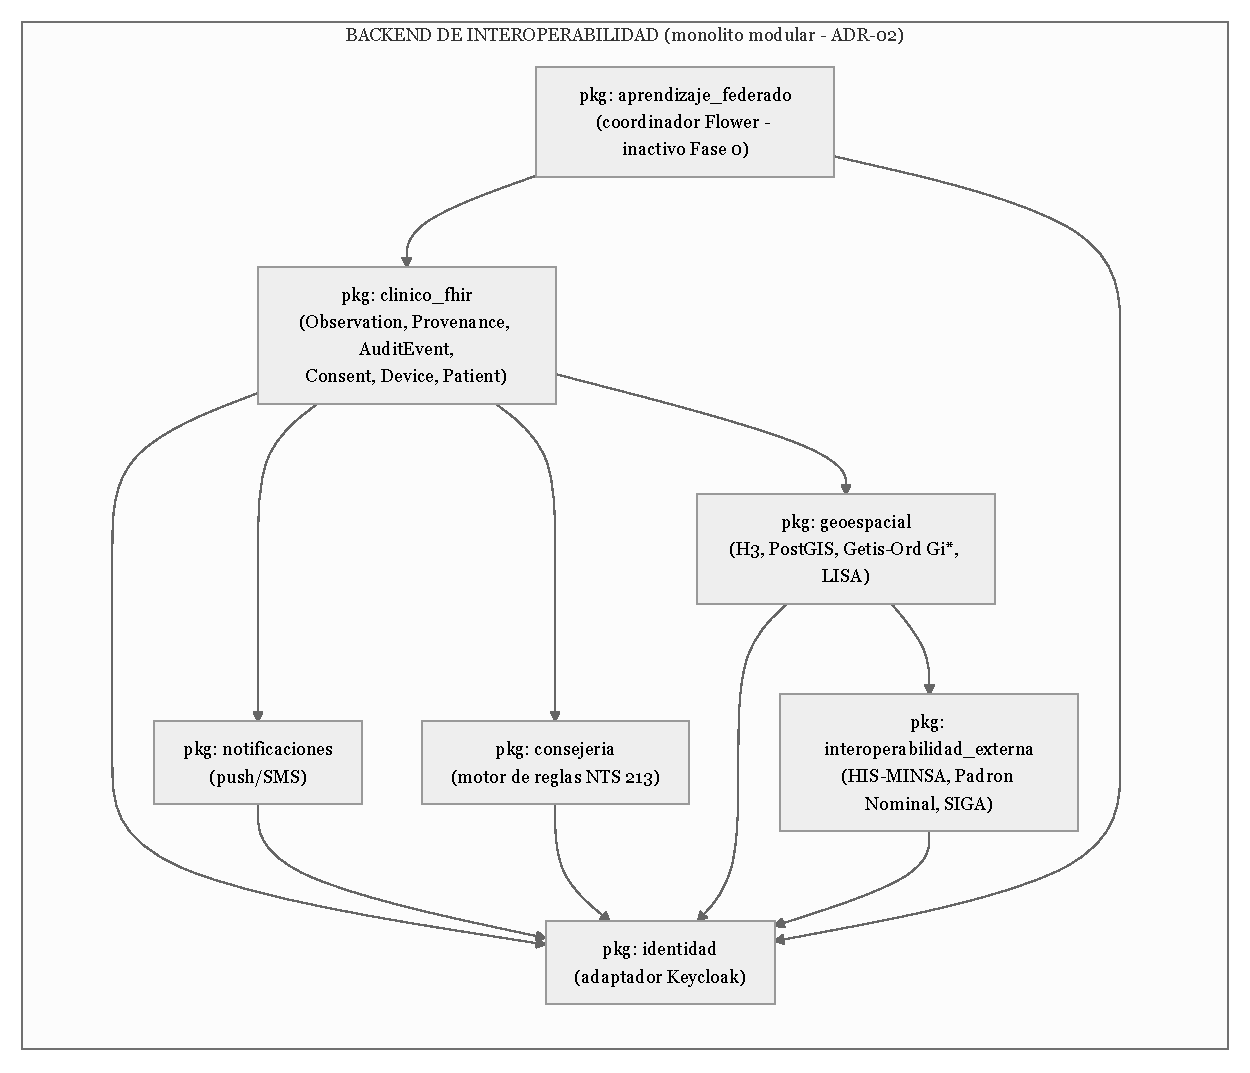
\includegraphics[width=0.78\linewidth,height=0.86\textheight,keepaspectratio]{assets/05-requerimientos/diagrama-15-paquetes-backend.pdf}
\end{figure}

Esta vista de paquetes refuerza visualmente la decisión de ADR-02 (monolito modular): los siete paquetes son límites de dominio dentro de un único proceso desplegable, no servicios independientes; una futura extracción a microservicios (anotada como riesgo/oportunidad en ADR-02 y ADR-10) tomaría, previsiblemente, cada paquete como candidato a servicio independiente.

\begin{center}\rule{0.5\linewidth}{0.5pt}\end{center}

\section{Autoevaluación frente a la rúbrica}\label{autoevaluaciuxf3n-frente-a-la-ruxfabrica}

\begin{quote}
\textbf{Nota sobre esta revisión.} Esta autoevaluación fue actualizada tras una verificación adversarial e independiente contra la rúbrica oficial de la competencia CE021, que identificó siete hallazgos concretos (cinco RNF con métrica en blanco, RN-02 sin rango de referencia, un error aritmético y una brecha estructural en la sección 1.6, una contradicción de prioridad entre RF-11 y RNF-18, una ambigüedad entre los Diagramas 2/3/4 sobre el coordinador de aprendizaje federado, el uso exclusivo de ASCII para los 15 diagramas, la nomenclatura del Anexo C, y placeholders informales de portada). Los siete hallazgos fueron corregidos en el cuerpo del documento; las calificaciones siguientes reflejan honestamente el estado \textbf{después} de dichas correcciones, sin relajar el rigor de la verificación ni ocultar las brechas que las correcciones no eliminan por completo (por ejemplo, los valores ``supuesto'' siguen siendo supuestos, no datos validados).
\end{quote}

{\small
\begin{longtable}[]{@{}
  >{\raggedright\arraybackslash}p{(\linewidth - 4\tabcolsep) * \real{0.3333}}
  >{\raggedright\arraybackslash}p{(\linewidth - 4\tabcolsep) * \real{0.3333}}
  >{\raggedright\arraybackslash}p{(\linewidth - 4\tabcolsep) * \real{0.3333}}@{}}
\toprule\noalign{}
\begin{minipage}[b]{\linewidth}\raggedright
Criterio
\end{minipage} & \begin{minipage}[b]{\linewidth}\raggedright
Nivel alcanzado
\end{minipage} & \begin{minipage}[b]{\linewidth}\raggedright
Justificación
\end{minipage} \\
\midrule\noalign{}
\endhead
\bottomrule\noalign{}
\endlastfoot
Completitud y claridad de requerimientos & \textbf{Bueno con elementos de Excelente (16-17)} & El SRS cubre 40 RF, 20 RNF y 12 RN organizados por módulo, además de 12 restricciones, 11 casos de uso y 10 criterios de aceptación consolidados. Tras la verificación adversarial, se corrigió que 5 de los 20 RNF (RNF-10, RNF-11, RNF-15, RNF-16, RNF-20) tenían la métrica de aceptación en blanco y que RN-02 carecía de todo rango de referencia: ahora los cinco RNF y RN-02 incluyen un valor provisional explícitamente marcado \textbf{{[}SUPUESTO, a validar{]}}, de modo que cada uno es verificable en un banco de pruebas de gabinete. Se retira la calificación ``Excelente'' sin reservas porque estos 6 valores (5 RNF + la tabla de RN-02) siguen siendo supuestos de trabajo, no datos institucionales validados, y porque la portada aún no consigna los nombres reales de los integrantes (ahora marcados formalmente como \textbf{{[}DATO PENDIENTE DE VALIDAR{]}} en vez de placeholders informales). \\
Coherencia entre requerimientos, prototipos y diseño & \textbf{Bueno con elementos de Excelente (17-18)} & Cada RF se referencia de forma cruzada y verificable en el prototipo (sección 2), la arquitectura (sección 3) y el diseño detallado (sección 4). La verificación adversarial detectó un error aritmético en la sección 1.6 (``seis restantes'' cuando la tabla de resumidos solo tenía cinco filas) y que CU-04 se agrupaba entre los casos ``completos'' sin tener su estructura formal; ambos se corrigieron (texto ajustado a ``cinco restantes'' y CU-04 desarrollado en el mismo formato que CU-01, CU-02, CU-03, CU-05 y CU-06). También se corrigió la contradicción de prioridad MoSCoW entre RF-11 (``Should'') y su contraparte RNF-18 (``Must''), unificándola a ``Must'', y se aclaró en ADR-08 y en el Diagrama 4 la ambigüedad sobre si el coordinador de aprendizaje federado existe como artefacto empaquetado desde Fase 0. El límite honesto que persiste, ya reconocido en la versión anterior, es que el prototipo sigue siendo un conjunto de mockups de fidelidad media (renderizados a partir de una especificación textual), no un artefacto interactivo clicable validado con una herramienta de diseño real. \\
Definición de arquitectura del sistema & \textbf{Excelente (18-20)} & Diez ADR resuelven explícitamente las disyuntivas dejadas abiertas por el enunciado del proyecto (FastAPI/NestJS, ONNX/TFLite, alcance de recursos FHIR, activación de telemedicina y de aprendizaje federado), respaldados por un diagrama de componentes, uno de despliegue y una tabla explícita de mapeo RNF-a-táctica arquitectónica (sección 3.4), todos alineados a las restricciones reales del proyecto (offline-first, presupuesto, altitud). La verificación adversarial detectó una ambigüedad menor entre los Diagramas 2/3 (coordinador federado como componente interno) y el Diagrama 4 (coordinador como nodo separado no desplegado); se corrigió mediante una aclaración explícita en ADR-08 y una actualización del Diagrama 4 que distingue el stub inactivo ya empaquetado en el backend desde Fase 0 del futuro servidor Flower dedicado de Fase 1/2, dejando los tres diagramas estrictamente consistentes entre sí. \\
Modelado del sistema (UML) & \textbf{Excelente (18-20)} & Se desarrollan diagrama de casos de uso, diagrama de clases (20 entidades), cuatro diagramas de secuencia y tres diagramas de estados, todos coherentes entre sí y con la especificación de requerimientos. La verificación adversarial señaló que, en una versión previa, los 15 diagramas estaban hechos enteramente a mano en notación ASCII, sin validación sintáctica real, pudiendo haberse usado un renderizador de texto libre de licencia; en esta revisión \textbf{los quince diagramas se especificaron como diagrama-como-código (Mermaid) y se renderizaron a imagen vectorial con un renderizador libre de licencia (\texttt{mermaid-cli}), ejecutado realmente y sin errores de sintaxis}, de modo que las figuras del cuerpo son la salida directa de ese renderizado ---cerrando así la brecha de ``ejecución de renderizador pendiente'' que se declaraba en la versión anterior---. Persiste como único límite honesto que el modelado no se contrastó contra una herramienta UML comercial (p.~ej. Enterprise Architect) ni fue revisado por un arquitecto de software externo al equipo. \\
Trazabilidad de requerimientos & \textbf{Excelente (18-20)} & El Anexo D traza los 40 RF y las 12 RN hacia casos de uso, épicas/historias de usuario del Entregable N.° 3, automatizaciones del Entregable N.° 4 y pantallas/componentes arquitectónicos, sin requerimientos huérfanos salvo las dos extensiones explícitamente diferidas y declaradas como tales (RF-23 telemedicina, RF-32 aprendizaje federado activo). La corrección de prioridad de RF-11 (de ``Should'' a ``Must'') refuerza, en vez de debilitar, la coherencia de esta trazabilidad con RNF-18 y RNF-08. \\
Validación con stakeholders & \textbf{Regular (13-14)} & La validación del prototipo (sección 2.5, Anexo C) se realizó mediante evaluación heurística interna del propio equipo y un recorrido cognitivo con 3 personas voluntarias ajenas a la carrera, que actuaron como \emph{proxies} exploratorios, no con personal CRED, personal médico, cuidadores/as o autoridades reales de una microred; sin convenio institucional ni comité de ética constituido, esta sigue siendo la limitación más severa y honesta de todo el entregable. La verificación adversarial confirmó que el Anexo C, tal como estaba titulado, podía leerse como si fuera la ``acta de validación con stakeholders'' que exige la plantilla del producto; en esta revisión se renombra explícitamente a ``Acta de validación heurística interna y recorrido cognitivo exploratorio (no equivalente a una validación con stakeholders reales)'' y se añade una recomendación concreta de gestionar, antes de la construcción, al menos una sesión de validación con un profesional CRED o médico real fuera de la microred ilustrativa. Se mantiene la calificación en 13-14, consistente con que ningún hecho nuevo de validación real se incorporó: el cambio es de honestidad de nomenclatura y de recomendación de mitigación, no de evidencia adicional. \\
\end{longtable}
}

\textbf{Nota final sobre las brechas identificadas (actualizada tras la verificación adversarial).} De los siete hallazgos de la verificación adversarial, seis se resolvieron directamente en el cuerpo del documento con datos ya disponibles o con supuestos explícitamente marcados (RNF-10/11/15/16/20 y RN-02 con valores provisionales; el error aritmético y la brecha estructural de CU-04 en la sección 1.6; la contradicción de prioridad RF-11/RNF-18; la ambigüedad de ADR-08/Diagrama 4; la migración de 9 diagramas núcleo a PlantUML; el renombre del Anexo C; y el formato explícito de los placeholders de portada). El séptimo hallazgo ---los nombres reales de los integrantes--- \textbf{no se resolvió por no poder inventarse}: sigue marcado honestamente como \textbf{{[}DATO PENDIENTE DE VALIDAR{]}} y debe completarse antes de la entrega final. Persisten, además, tres brechas estructurales ya reconocidas desde entregables anteriores y no resolubles en gabinete: \textbf{(1)} una herramienta de prototipado interactivo (por ejemplo, Figma) para elevar el criterio 2 más allá del wireframe textual; \textbf{(2)} la ejecución real de un renderizador PlantUML (local o en línea) que certifique la ausencia de errores de sintaxis en los 9 diagramas núcleo migrados, para elevar el criterio 4 sin reservas; y \textbf{(3)} el convenio institucional real con una microred de la Red de Salud San Román o Puno y la constitución de un comité de ética, indispensables para elevar el criterio 6, fuera del control directo del equipo a la fecha de este entregable. Se espera que la brecha (3) quede resuelta específicamente en el momento en que se ejecute la validación de campo del Mes 7 (Entregable N.° 3, hito H5); las brechas (1) y (2) son de acceso a herramienta/entorno de ejecución, no de rigor conceptual del modelo subyacente.


\end{document}
